\documentclass[11pt,a4paper]{elsarticle} %review=doublespace preprint=single 5p=2 column
%%% Begin My package additions %%%%%%%%%%%%%%%%%%%
\usepackage[hyphens]{url}

  \journal{International Journal of Forecasting} % Sets Journal name


\usepackage{lineno} % add
\providecommand{\tightlist}{%
  \setlength{\itemsep}{0pt}\setlength{\parskip}{0pt}}

\bibliographystyle{elsarticle-harv}
\biboptions{sort&compress} % For natbib
\usepackage{graphicx}
\usepackage{booktabs} % book-quality tables
%%%%%%%%%%%%%%%% end my additions to header

\usepackage[T1]{fontenc}
\usepackage{lmodern}
\usepackage{amssymb,amsmath}
\usepackage{ifxetex,ifluatex}
\usepackage{fixltx2e} % provides \textsubscript
% use upquote if available, for straight quotes in verbatim environments
\IfFileExists{upquote.sty}{\usepackage{upquote}}{}
\ifnum 0\ifxetex 1\fi\ifluatex 1\fi=0 % if pdftex
  \usepackage[utf8]{inputenc}
\else % if luatex or xelatex
  \usepackage{fontspec}
  \ifxetex
    \usepackage{xltxtra,xunicode}
  \fi
  \defaultfontfeatures{Mapping=tex-text,Scale=MatchLowercase}
  \newcommand{\euro}{€}
\fi
% use microtype if available
\IfFileExists{microtype.sty}{\usepackage{microtype}}{}
\usepackage[margin=1.5cm]{geometry}
\ifxetex
  \usepackage[setpagesize=false, % page size defined by xetex
              unicode=false, % unicode breaks when used with xetex
              xetex]{hyperref}
\else
  \usepackage[unicode=true]{hyperref}
\fi
\hypersetup{breaklinks=true,
            bookmarks=true,
            pdfauthor={},
            pdftitle={International Journal of Forecasting 1985-2018: A retrospective based on bibliometric and knowledge diffusion analysis},
            colorlinks=false,
            urlcolor=blue,
            linkcolor=magenta,
            pdfborder={0 0 0}}
\urlstyle{same}  % don't use monospace font for urls

\setcounter{secnumdepth}{5}
% Pandoc toggle for numbering sections (defaults to be off)
% Pandoc header
%% FONT and LAYOUT
\usepackage{mathpazo}
\usepackage{parskip}

%% CAPTIONS
\usepackage{caption}
\DeclareCaptionStyle{italic}[justification=centering]
 {labelfont={bf},textfont={it},labelsep=colon}
\captionsetup[figure]{style=italic,format=hang,singlelinecheck=true}
\captionsetup[table]{style=italic,format=hang,singlelinecheck=true}

%% MATHS
\usepackage{bm}
\allowdisplaybreaks

%% GRAPHICS
\usepackage[section]{placeins}
\setcounter{topnumber}{2}
\setcounter{bottomnumber}{2}
\setcounter{totalnumber}{4}
\renewcommand{\topfraction}{0.85}
\renewcommand{\bottomfraction}{0.85}
\renewcommand{\textfraction}{0.15}
\renewcommand{\floatpagefraction}{0.7}
\usepackage{mathpazo}
\usepackage{parskip}
\usepackage{lscape}
\usepackage{graphicx}
\usepackage{subfigure}
\usepackage{float}
\usepackage{rotating}
\usepackage{rotate}
\usepackage{makecell}
\usepackage{geometry}
\usepackage{indentfirst}

\newcommand{\tablea}
{\begin{table}[!htbp]
\centering
\caption{Information about top 20 most cited IJF papers}
\setlength{\tabcolsep}{3.5mm}{
\begin{tabular}{ccccccc}
\hline
Rank & Paper & TC & TC/Year & Country & Nau & Nin\\
\hline
1 & ZHANG et al. (1998) & 2007 & 95.57 & USA & 3 & 1\\
2 & HYNDMAN and KOEHLER (2006) & 1198 & 92.15 & Australia & 2 & 2\\
3 & CLEMEN (1989) & 1105 & 36.83 & USA & 1 & 1\\
4 & ROWE and WRIGHT (1999) & 941 & 47.05 & UK & 2 & 2\\
5 & MAKRIDAKIS and HIBON (2000) & 669 & 35.21 & France & 2 & 1\\
6 & DE GOOIJER and HYNDMAN (2006) & 612 & 47.08 & Netherlands & 2 & 2\\
7 & ARMSTRONG and COLLOPY (1992) & 573 & 21.22 & USA & 2 & 2\\
8 & HARVEY et al. (1997) & 564 & 25.64 & UK & 3 & 1\\
9 & WITT and WITT (1995) & 468 & 19.50 & UK & 2 & 2\\
10 & THOMAS (2000) & 390 & 20.53 & UK & 1 & 1\\
11 & MEADE and ISLAM (2006) & 381 & 29.31 & UK & 2 & 2\\
12 & GARDNER (2006) & 377 & 29.00 & USA & 1 & 1\\
13 & DIEBOLD and YILMAZ (2012) & 375 & 53.57 & USA & 2 & 3\\
14 & HOLT (2004) & 372 & 24.80 & USA & 1 & 1\\
15 & WERON (2014) & 345 & 69.00 & Poland & 1 & 1\\
16 & HYNDMAN et al. (2002) & 310 & 18.24 & Australia & 4 & 2\\
17 & CONEJO et al, (2005) & 282 & 20.14 & Spain & 4 & 2\\
18 & TAYLOR et al., (2006) & 265 & 20.38 & UK & 3 & 3\\
19 & BROWN (1993) & 221 & 8.50 & USA & 1 & 1\\
20 & LAWRENCE (2006) & 212 & 16.31 & Australia & 4 & 4\\
\hline
\end{tabular}}
\end{table}}

\newcommand{\tableb}
{\begin{table}[!htbp]
\centering
\caption{Information about the most local cited IJF papers}
\setlength{\tabcolsep}{7mm}{
\begin{tabular}{ccccc}
\hline
Rank & Paper & LC & TC & LC/ TC\\
\hline
1 & DE GOOIJER and HYNDMAN (2006) & 33 & 612 & 5.39\%\\
2 & WERON (2014) & 17 & 345 & 4.93\%\\
3 & GARDNER (2006) & 16 & 377 & 4.24\%\\
4 & MAKRIDAKIS and HIBON (2000) & 16 & 669 & 2.39\%\\
5 & ZHANG et al. (1998) & 12 & 2007 & 0.60\%\\
6 & CLEMEN (1989) & 11 & 1105 & 1.00\%\\
7 & CRONE et al. (2011) & 10 & 108 & 9.26\%\\
8 & TAYLOR et al. (2008) & 10 & 124 & 8.06\%\\
9 & LAWRENCE et al. (2006) & 10 & 212 & 4.72\%\\
10 & DARBELLAY and SLAMA (2000) & 10 & 207 & 4.83\%\\
11 & MAKRIDAKIS (1993) & 10 & 133 & 7.52\%\\
\hline
\end{tabular}}
\end{table}}

\newcommand{\tablec}
{\begin{table}[!htbp]
\centering
\caption{Information about the most co-cited papers in the co-citation network}
\setlength{\tabcolsep}{0.3mm}{
\begin{tabular}{c c c c c c c c c c}
\hline
Rank & Co & Paper & Source &    FY &    LY &    Y & best year (number) &    Ave-Co &    Citation\\
\hline
1 & 26 & TIMMERMANN (2006) & HEF & 2009 & 2014 & 6 & 2009(9) & 4.33 & 1247\\
2 & 24 & GIACOMINI and WHITE (2006) & Econometrica & 2007 & 2014 & 8 & 2009/2011/2013(5) & 3.00 & 1231\\
3 & 22 & MAKRIDAKIS and HIBON (2000) & IJF & 2003 & 2008 & 6 & 2006(7) & 3.67 & 1325\\
4 & 20 & HANSEN et al. (2011) & Econometrica & 2012 & 2018 & 7 & 2018(7) & 2.86 & 1036\\
5 & 18 & GIANNONE et al. (2008) & JME & 2013 & 2018 & 6 & 2016(8) & 3.00 & 793\\
6 & 17 & HYNDMAN and KOEHLER (2006) & IJF & 2009 & 2014 & 6 & 2011(6) & 2.83 & 2338\\
7 & 16 & ARMSTRONG (2001) & PF: AHRP & 2001 & 2007 & 7 & 2002/2006(6) & 2.28 & 1740\\
8 & 15 & FILDES et al. (2009) & IJF & 2011 & 2017 & 7 & 2013(7) & 2.14 & 299\\
9 & 14 & HONG et al. (2016) & IJF & 2016 & 2018 & 3 & 2016(8) & 4.67 & 251\\
10 & 14 & LAWRENCE (2006) & JACC & 2007 & 2013 & 7 & 2013(6) & 2.00 & 379\\
\hline
\end{tabular}}
\end{table}}

\newcommand{\tabled}
{\begin{table}[!htbp]
\centering
\caption{Information about the top ten prolific authors in IJF}
\setlength{\tabcolsep}{2.7mm}{
\begin{tabular}{ccccccccccc}
\hline
Rank & Author & TP & Country & FY & LY & Y & 1st & 1st \% & Cor & Cor \%\\
\hline
1 & ARMSTRONG JS & 50 & USA & 1985 & 2014 & 30 & 35 & 70.00\% & 34 & 68.00\%\\
2 & FILDES R & 42 & UK & 1985 & 2017 & 33 & 31 & 73.81\% & 31 & 73.81\%\\
3 & FRANSES PH & 26 & Netherlands & 1991 & 2017 & 27 & 12 & 46.15\% & 13 & 50.00\%\\
4 & HYNDMAN RJ & 24 & Australia & 1992 & 2018 & 27 & 11 & 45.83\% & 13 & 54.17\%\\
5 & STEKLER HO & 24 & USA & 1988 & 2015 & 28 & 10 & 41.67\% & 12 & 50.00\%\\
6 & GOODWIN P & 22 & UK & 1993 & 2017 & 25 & 10 & 45.45\% & 13 & 59.09\%\\
7 & MAKRIDAKIS S & 22 & Cyprus & 1985 & 2018 & 34 & 17 & 77.27\% & 15 & 68.18\%\\
8 & CLEMENTS MP & 20 & UK & 1997 & 2018 & 22 & 18 & 90.00\% & 11 & 55.00\%\\
9 & KOEHLER AB & 19 & USA & 1985 & 2017 & 33 & 6 & 31.58\% & 10 & 52.63\%\\
10 & O'CONNOR M & 18 & Australia & 1989 & 2007 & 19 & 5 & 27.78\% & 7 & 38.89\%\\
\hline
\end{tabular}}
\end{table}}

\newcommand{\tablee}
{\begin{table}[!htbp]
\centering
\caption{Information about the top ten most cited IJF authors}
\setlength{\tabcolsep}{4.3mm}{
\begin{tabular}{ccccccccc}
\hline
Rank & Author & TC & TP & TC/TP & LC & \% & OC & \%\\
\hline
1 & HYNDMAN RJ & 2547 & 24 & 106.13 & 121 & 4.75\% & 2426 & 95.25\%\\
2 & ZHANG G & 2075 & 1 & 2075.00 & 27 & 1.30\% & 2048 & 98.70\%\\
3 & KOEHLER AB & 1728 & 19 & 90.95 & 82 & 4.75\% & 1646 & 95.25\%\\
4 & ARMSTRONG JS & 1514 & 44 & 34.41 & 149 & 9.84\% & 1365 & 90.16\%\\
5 & MAKRIDAKIS S & 1338 & 22 & 60.82 & 178 & 13.30\% & 1160 & 86.70\%\\
6 & WRIGHT G & 1217 & 9 & 135.22 & 47 & 3.86\% & 1170 & 96.14\%\\
7 & CLEMEN RT & 1182 & 6 & 197.00 & 107 & 9.05\% & 1075 & 90.95\%\\
8 & HIBON M & 1057 & 11 & 96.09 & 140 & 13.25\% & 917 & 86.75\%\\
9 & ROWE G & 1027 & 3 & 342.33 & 20 & 1.95\% & 1007 & 98.05\%\\
10 & DE GOOIJER JG & 770 & 9 & 85.56 & 31 & 4.03\% & 739 & 95.97\%\\
\hline
\end{tabular}}
\end{table}}

\newcommand{\tablef}
{\begin{table}
\centering
\caption{Information about the top ten prolific countries}
\setlength{\tabcolsep}{6mm}{
\begin{tabular}{cccccccc}
\hline
Rank & Country & TP & FY & LY & Y & TP/Y & \% of total\\
\hline
1 & USA & 798 & 1985 & 2018 & 34 & 23.47 & 41.18\%\\
2 & UK & 420 & 1985 & 2018 & 34 & 12.35 & 21.67\%\\
3 & Australia & 178 & 1985 & 2018 & 34 & 5.24 & 9.18\%\\
4 & Germany & 110 & 1988 & 2018 & 31 & 3.55 & 5.68\%\\
5 & Netherlands & 99 & 1988 & 2018 & 31 & 3.19 & 5.11\%\\
6 & Spain & 93 & 1986 & 2018 & 33 & 2.82 & 4.80\%\\
7 & Canada & 84 & 1985 & 2018 & 34 & 2.47 & 4.33\%\\
8 & Italy & 70 & 1987 & 2018 & 32 & 2.19 & 3.61\%\\
9 & France & 67 & 1986 & 2018 & 33 & 2.03 & 3.46\%\\
10 & Belgium & 36 & 1989 & 2018 & 30 & 1.20 & 1.86\%\\
\hline
\end{tabular}}
\end{table}}

\newcommand{\tableg}
{\begin{table}
\centering
\caption{Information about the top ten most cited countries}
\setlength{\tabcolsep}{4mm}{
\begin{tabular}{ccccccccc}
\hline
Rank & Country & TC & TP & TC/TP & In-TC & In\% & Out-TC & Out\%\\
\hline
1 & USA & 22875 & 798 & 28.67 & 901 & 3.94\% & 21974 & 96.06\%\\
2 & UK & 12899 & 420 & 30.71 & 646 & 5.01\% & 12253 & 94.99\%\\
3 & Australia & 6540 & 178 & 36.74 & 352 & 5.38\% & 6188 & 94.62\%\\
4 & Netherlands & 2635 & 99 & 26.62 & 150 & 5.69\% & 2485 & 94.31\%\\
5 & France & 2417 & 67 & 36.07 & 226 & 9.35\% & 2191 & 90.65\%\\
6 & Germany & 2023 & 110 & 18.39 & 164 & 8.11\% & 1859 & 91.89\%\\
7 & Spain & 1876 & 93 & 20.17 & 128 & 6.82\% & 1748 & 93.18\%\\
8 & Canada & 1850 & 84 & 22.02 & 121 & 6.54\% & 1729 & 93.46\%\\
9 & Italy & 1122 & 70 & 16.03 & 122 & 10.87\% & 1000 & 89.13\%\\
10 & turkey & 1061 & 33 & 32.15 & 57 & 5.37\% & 1004 & 94.63\%\\
\hline
\end{tabular}}
\end{table}}

\newcommand{\tableh}
{\begin{table}
\centering
\caption{Information about the countries in the country collaboration network}
\setlength{\tabcolsep}{7mm}{
\begin{tabular}{cccccc}
\hline
Rank & Country & Link & CM & Number & N/L\\
\hline
1 & USA & 217 & UK & 44 & 20.28\%\\
2 & UK & 201 & USA & 44 & 21.89\%\\
3 & Australia & 116 & US & 42 & 36.21\%\\
4 & Netherlands & 69 & USA/Belgium & 8 & 11.59\%\\
5 & Germany & 61 & USA & 14 & 22.95\%\\
6 & Italy & 57 & UK & 21 & 36.84\%\\
7 & Canada & 54 & USA & 19 & 35.19\%\\
8 & France & 49 & UK & 15 & 30.61\%\\
9 & Spain & 39 & UK & 13 & 33.33\%\\
10 & Belgium & 34 & Netherlands/UK & 8 & 23.53\%\\
11 & Denmark & 32 & Netherlands & 7 & 21.88\%\\
12 & Turkey & 30 & UK & 12 & 40.00\%\\
13 & Switzerland & 20 & USA & 4 & 20.00\%\\
14 & Brazil & 19 & UK & 6 & 31.58\%\\
15 & China & 19 & USA & 9 & 47.37\%\\
16 & Sweden & 15 & Netherlands & 4 & 26.67\%\\
17 & Taiwan & 14 & USA & 5 & 35.71\%\\
18 & Norway & 12 & Italy & 4 & 33.33\%\\
19 & Greece & 11 & UK & 6 & 54.55\%\\
20 & New Zealand & 11 & USA & 6 & 54.55\%\\
21 & South Korea & 11 & USA & 8 & 72.73\%\\
22 & Austria & 10 & Germany & 5 & 50.00\%\\
23 & Japan & 10 & USA/Japan & 3 & 30.00\%\\
24 & Portugal & 8 & Spain/USA & 3 & 37.50\%\\
25 & Finland & 7 & Sweden/UK/USA & 2 & 28.57\%\\
\hline
\end{tabular}}
\end{table}}

\newcommand{\tablei}
{\begin{table}[!htbp]
	\centering
	\caption{Information about the top ten most prolific subject areas}
	\setlength{\tabcolsep}{1.1mm}{
	\begin{tabular}{c c c c|c c c c}
		\hline
		\multicolumn{4}{c|}{29464 citing papers of IJF} & \multicolumn{4}{c}{16419 citing papers of JF}\\
		\hline
		Rank & Subject area & NP1 & Percent1 & Rank & Subject area & NP2 & Percent2\\
		\hline
		1 & Computer Science & 7586 & 25.75\% & 1 & \makecell[c]{Economics, Econometrics \\ and Finance} & 5184 & 31.57\%\\
		2 & \makecell[c]{Economics, Econometrics \\ and Finance} & 7487 & 25.41\% & 2 & \makecell[c]{Business, Management \\ and Accounting} & 4891 & 29.79\%\\
    3 & \makecell[c]{Business, Management \\ and Accounting} & 7449 & 25.28\% & 3 & Mathematics & 3946 & 24.03\%\\
    4 & Engineering & 5888 & 19.98\% & 4 & Computer Science & 3791 & 23.09\%\\
    5 & Mathematics & 5482 & 18.61\% & 5 & Decision Sciences & 2971 & 18.09\%\\
    6 & Social Sciences & 4277 & 14.52\% & 6 & Engineering & 2305 & 14.04\%\\
    7 & Decision Sciences & 3665 & 12.44\% & 7 & Social Sciences & 2179 & 13.27\%\\
    8 & Energy & 2222 & 7.54\% & 8 & Environmental Science & 1109 & 6.75\%\\
    9 & Environmental Science & 2070 & 7.03\% & 9 & Energy & 641 & 3.90\%\\
    10 & Earth and Planetary Sciences & 969 & 3.29\% & 10 & Earth and Planetary Sciences & 588 & 3.58\%\\
		\hline
	\end{tabular}}
\end{table}}

\newcommand{\tablej}
{\begin{table}[!htbp]
\centering
\caption{Information about the IJF journal citation network in Computer Science }
\setlength{\tabcolsep}{0.5mm}{
\begin{tabular}{ccccc}
\hline
Rank & Journal & Links & Links with IJF & \%\\
\hline
1 & Journal of Forecasting & 1814 & 1464 & 80.71\%\\
2 & Expert Systems with Applications & 1279 & 553 & 43.24\%\\
3 & Neurocomputing & 686 & 259 & 37.76\%\\
4 & European Journal of Operational Research & 647 & 462 & 71.41\%\\
5 & Lecture Notes in Computer Science & 609 & 444 & 72.91\%\\
6 & Applied Soft Computing & 446 & 160 & 35.87\%\\
7 & Decision Support Systems & 345 & 149 & 43.19\%\\
8 & Computational Statistics and Data Analysis & 341 & 214 & 62.76\%\\
9 & Neuro Computing and Application & 286 & 99 & 34.62\%\\
10 & Proceedings of The International Joint Conference on Neural Networks & 260 & 173 & 66.54\%\\
\hline
\end{tabular}}
\end{table}}

\newcommand{\tablek}
{\begin{table}[!htbp]
\centering
\caption{Information about the IJF journal citation network in Economics, Econometrics and Finance}
\setlength{\tabcolsep}{4.5mm}{
\begin{tabular}{ccccc}
\hline
Rank & Journal & Links & Links with IJF & \%\\
\hline
1 & Journal of business and economic statistics & 1535 & 638 & 41.56\%\\
2 & Journal of Economics & 1227 & 497 & 40.51\%\\
3 & Journal of Applied Economics & 908 & 350 & 38.55\%\\
4 & Applied Economics & 891 & 459 & 51.52\%\\
5 & Energy Economics & 890 & 454 & 51.01\%\\
6 & Economic Modeling & 836 & 346 & 41.39\%\\
7 & Empirical Economics & 656 & 311 & 47.41\%\\
8 & Oxford Bulletin of Economics and Statistics & 436 & 184 & 42.20\%\\
9 & International Journal of Production Economics & 423 & 403 & 95.27\%\\
10 & Journal of Empirical Finance & 336 & 121 & 36.01\%\\
\hline
\end{tabular}}
\end{table}}

\newcommand{\tablel}
{\begin{table}[!htbp]
\centering
\caption{Information about the IJF journal citation network in Business, Management and Accounting}
\setlength{\tabcolsep}{3mm}{
\begin{tabular}{ccccc}
\hline
Rank & Journal & Links & Links with IJF & \%\\
\hline
1 & Journal of Forecasting & 1891 & 1547 & 81.81\%\\
2 & Tourism Management & 981 & 219 & 22.32\%\\
3 & Tourism Economics & 921 & 275 & 29.86\%\\
4 & International Journal of Production Economics & 785 & 421 & 53.63\%\\
5 & Journal of Travel Research & 721 & 162 & 22.47\%\\
6 & Journal of the Operational Research Society & 709 & 387 & 54.58\%\\
7 & Technological Forecasting and Social Change & 612 & 431 & 70.42\%\\
8 & Annals of Tourism Research & 591 & 116 & 19.63\%\\
9 & Organizational Behavior and Human Decision Processes & 412 & 193 & 46.84\%\\
10 & Omega & 378 & 208 & 55.03\%\\
\hline
\end{tabular}}
\end{table}}

\newcommand{\tablem}
{\begin{table}[!htbp]
\centering
\caption{Information about the JF journal citation network in Business, Management and Accounting}
\setlength{\tabcolsep}{3mm}{
\begin{tabular}{ccccc}
\hline
Rank & Journal & Links & Links with IJF & \%\\
\hline
1 & Journal of Forecasting & 3391 & 1887 & 55.65\%\\
2 & Technological Forecasting and Social Change & 411 & 172 & 41.85\%\\
3 & International Journal of Production Economics & 408 & 113 & 27.70\%\\
4 & Journal of the Operational Research Society & 351 & 146 & 41.60\%\\
5 & Tourism Management & 327 & 70 & 21.41\%\\
6 & Organizational Behavior and Human Decision Processes & 316 & 68 & 21.52\%\\
7 & Tourism Economics & 309 & 51 & 16.50\%\\
8 & Omega & 299 & 80 & 26.76\%\\
9 & Journal of Behavioral Decision Making & 225 & 69 & 30.67\%\\
10 & Annals of Tourism Research & 213 & 48 & 22.54\%\\
\hline
\end{tabular}}
\end{table}}

\newcommand{\tablen}
{\begin{table}[!htbp]
\centering
\caption{Information about the JF journal citation network in Economics, Econometrics and Finance}
\setlength{\tabcolsep}{5mm}{
\begin{tabular}{ccccc}
\hline
Rank & Journal & Links & Links with IJF & \%\\
\hline
1 & Journal of Business and Economic Statistics & 1319 & 549 & 41.62\%\\
2 & Journal of Econometrics & 1104 & 408 & 36.96\%\\
3 & Journal of Applied Econometrics & 755 & 232 & 30.73\%\\
4 & Economic Modelling & 615 & 250 & 40.65\%\\
5 & Energy Economics & 509 & 193 & 37.92\%\\
6 & Empirical Economics & 502 & 230 & 45.82\%\\
7 & Applied Economics & 466 & 236 & 50.64\%\\
8 & Oxford Bulletin of Economics and Statistics & 369 & 142 & 38.48\%\\
9 & Econometric Reviews & 285 & 100 & 35.09\%\\
10 & Journal of Empirical Finance & 267 & 93 & 34.83\%\\
\hline
\end{tabular}}
\end{table}}

\newcommand{\tableo}
{\begin{table}[!htbp]
\centering
\caption{Information about the JF journal citation network in Mathematics}
\setlength{\tabcolsep}{4mm}{
\begin{tabular}{ccccc}
\hline
Rank & Journal & Links & Links with IJF & \%\\
\hline
1 & Journal of Business and Economic Statistics & 978 & 563 & 57.57\%\\
2 & Empirical Economics & 405 & 231 & 57.04\%\\
3 & Journal of Econometrics & 385 & 201 & 52.21\%\\
4 & European Journal of Operational Research & 327 & 248 & 75.84\%\\
5 & Computational Statistics and Data Analysis & 301 & 154 & 51.16\%\\
6 & Journal of the American Statistical Association & 286 & 143 & 50.00\%\\
7 & Oxford Bulletin of Economics and Statistics & 255 & 144 & 56.47\%\\
8 & Journal of Applied Statistics & 251 & 176 & 70.12\%\\
9 & Journal of Time Series Analysis & 205 & 109 & 53.17\%\\
10 & Studies in Nonlinear Dynamics and Econometrics & 179 & 98 & 54.75\%\\
\hline
\end{tabular}}
\end{table}}

\newcommand{\tablep}
{\begin{table}[!htbp]
\centering
\caption{Information about the IJF journal citation network in Engineering}
\setlength{\tabcolsep}{2.2mm}{
\begin{tabular}{ccccc}
\hline
Rank & Journal & Links & Links with IJF & \%\\
\hline
1 & Expert Systems with Applications & 797 & 543 & 68.13\%\\
2 & Energies & 693 & 319 & 46.03\%\\
3 & Energy & 609 & 262 & 43.02\%\\
4 & Applied Energy & 595 & 209 & 35.13\%\\
5 & IEEE Transactions on Power Systems & 553 & 196 & 35.44\%\\
6 & International Journal of Production Economics & 513 & 403 & 78.56\%\\
7 & International Journal of Electrical Power and Energy Systems & 287 & 98 & 34.15\%\\
8 & Transportation Research Part C: Emerging Technologies & 233 & 63 & 27.04\%\\
9 & Mathematical Problems in Engineering & 203 & 106 & 52.22\%\\
10 & Electric Power Systems Research & 193 & 57 & 29.53\%\\
\hline
\end{tabular}}
\end{table}}

\newcommand{\tableq}
{\begin{table}[!htbp]
\centering
\caption{Information about the IJF journal citation network in Mathematics}
\setlength{\tabcolsep}{4.6mm}{
\begin{tabular}{ccccc}
\hline
Rank & Journal & Links & Links with IJF & \%\\
\hline
1 & Journal of Forecasting & 2317 & 1464 & 63.19\%\\
2 & Journal of Business and Economic Statistics & 1290 & 638 & 49.46\%\\
3 & European Journal of Operational Research & 1002 & 757 & 75.55\%\\
4 & Empirical Economics & 608 & 311 & 51.15\%\\
5 & Lecture Notes in Computer Science & 525 & 444 & 84.57\%\\
6 & Journal of Econometrics & 463 & 205 & 44.28\%\\
7 & Computational Statistics and Data Analysis & 407 & 214 & 52.58\%\\
8 & Energies & 394 & 319 & 80.96\%\\
9 & Oxford Bulletin of Economics and Statistics & 363 & 184 & 50.69\%\\
10 & Journal of the American Statistical Association & 358 & 196 & 54.75\%\\
\hline
\end{tabular}}
\end{table}}

\newcommand{\tabler}
{\begin{table}[!htbp]
\centering
\caption{Information about the IJF journal citation network in Social Sciences}
\setlength{\tabcolsep}{0.8mm}{
\begin{tabular}{ccccc}
\hline
Rank & Journal & Links & Links with IJF & \%\\
\hline
1 & Tourism Management & 1016 & 214 & 21.06\%\\
2 & Journal of Business and Economic Statistics & 1012 & 638 & 63.04\%\\
3 & Tourism Economics & 932 & 275 & 29.51\%\\
4 & Journal of Travel Research & 752 & 161 & 21.41\%\\
5 & Journal of Applied Econometrics & 640 & 350 & 54.69\%\\
6 & Annals of Tourism Research & 598 & 116 & 19.40\%\\
7 & Empirical Economics & 514 & 311 & 60.51\%\\
8 & Oxford Bulletin of Economics and Statistics & 309 & 184 & 59.55\%\\
9 & Journal of the Royal Statistical Society. series a: statistics in society & 183 & 93 & 50.82\%\\
10 & International Journal of Tourism Research & 177 & 27 & 15.25\%\\
\hline
\end{tabular}}
\end{table}}

\newcommand{\tables}
{\begin{table}[!htbp]
\centering
\caption{Information about the IJF journal citation network in Decision Sciences}
\setlength{\tabcolsep}{4.5mm}{
\begin{tabular}{ccccc}
\hline
Rank & Journal & Links & Links with IJF & \%\\
\hline
1 & Journal of Forecasting & 2161 & 1464 & 67.75\%\\
2 & European Journal of Operational Research & 1401 & 757 & 54.03\%\\
3 & Journal of Business and Economic Statistics & 1061 & 638 & 60.13\%\\
4 & International Journal of Production Economics & 914 & 397 & 43.44\%\\
5 & Journal of the Operational Research Society & 860 & 369 & 42.91\%\\
6 & Omega & 413 & 205 & 49.64\%\\
7 & Journal of Behavioral Decision Making & 306 & 166 & 54.25\%\\
8 & Journal of the American Statistical Association & 301 & 183 & 60.80\%\\
9 & Oxford Bulletin of Economics and Statistics & 298 & 181 & 60.74\%\\
10 & Decision Support Systems & 289 & 149 & 51.56\%\\
\hline
\end{tabular}}
\end{table}}

\newcommand{\tablet}
{\begin{table}[!htbp]
\centering
\caption{Information about the IJF journal citation network in Energy}
\setlength{\tabcolsep}{2mm}{
\begin{tabular}{ccccc}
\hline
Rank & Journal & Links & Links with IJF & \%\\
\hline
1 & Energies & 967 & 332 & 34.33\%\\
2 & Energy Economics & 896 & 454 & 50.67\%\\
3 & Applied Energy & 886 & 209 & 23.59\%\\
4 & Renewable and Sustainable Energy Reviews & 839 & 183 & 21.81\%\\
5 & IEEE Transactions on Power Systems & 671 & 196 & 29.21\%\\
6 & Energy Conversion and Management & 474 & 92 & 19.41\%\\
7 & Renewable Energy & 374 & 83 & 22.19\%\\
8 & International Journal of Electrical Power and Energy Systems & 341 & 98 & 28.74\%\\
9 & Energy Policy & 336 & 128 & 38.10\%\\
10 & Energy & 311 & 71 & 22.83\%\\
\hline
\end{tabular}}
\end{table}}

\newcommand{\tableu}
{\begin{table}[!htbp]
\centering
\caption{Information about the IJF journal citation network in Environmental Science}
\setlength{\tabcolsep}{6mm}{
\begin{tabular}{ccccc}
\hline
Rank & Journal & Links & Links with IJF & \%\\
\hline
1 & Energy & 472 & 286 & 60.59\%\\
2 & Applied Energy & 339 & 190 & 56.05\%\\
3 & Energy Policy & 196 & 128 & 65.31\%\\
4 & Journal of Hydrology & 147 & 72 & 48.98\%\\
5 & Sustainability & 146 & 107 & 73.29\%\\
6 & Environmental Modelling and Software & 103 & 58 & 56.31\%\\
7 & Journal of Cleaner Production & 63 & 45 & 71.43\%\\
8 & Water Resources Research & 57 & 33 & 57.89\%\\
9 & Journal of Hydrologic Engineering & 53 & 30 & 56.60\%\\
10 & Water Resources Management & 50 & 29 & 58.00\%\\
\hline
\end{tabular}}
\end{table}}

\newcommand{\tablev}
{\begin{table}[!htbp]
\centering
\caption{Information about the IJF journal citation network in Earth and Planetary Sciences}
\setlength{\tabcolsep}{3.3mm}{
\begin{tabular}{ccccc}
\hline
Rank & Journal & Links & Links with IJF & \%\\
\hline
1 & Weather and Forecasting & 119 & 49 & 41.18\%\\
2 & Monthly Weather Review & 76 & 32 & 42.11\%\\
3 & Meteorological Applications & 65 & 22 & 33.85\%\\
4 & Quarterly Journal of the Royal Meteorological Society & 52 & 25 & 48.08\%\\
5 & Journal of Climate & 48 & 23 & 47.92\%\\
6 & International Journal of Climatology & 36 & 17 & 47.22\%\\
7 & Climate Dynamics & 35 & 14 & 40.00\%\\
8 & Bulletin of the American Meteorological Society & 34 & 12 & 35.29\%\\
9 & Hydrology and Earth System Sciences & 27 & 14 & 51.85\%\\
10 & Geographical Analysis & 26 & 25 & 96.15\%\\
\hline
\end{tabular}}
\end{table}}

\newcommand{\tablew}
{\begin{table}[!htbp]
\centering
\caption{Information about the JF journal citation network in Computer Science}
\setlength{\tabcolsep}{5.1mm}{
\begin{tabular}{ccccc}
\hline
Rank & Journal & Links & Links with IJF & \%\\
\hline
1 & Expert Systems with Applications & 381 & 169 & 44.36\%\\
2 & Neurocomputing & 266 & 90 & 33.83\%\\
3 & European Journal of Operational Research & 208 & 136 & 65.38\%\\
4 & Computational Statistics and Data Analysis & 186 & 154 & 82.80\%\\
5 & Lecture Notes in Computer Science & 183 & 133 & 72.68\%\\
6 & Applied Soft Computing Journal & 169 & 58 & 34.32\%\\
7 & Computers and Operations Research & 161 & 51 & 31.68\%\\
8 & Decision Support Systems & 148 & 59 & 39.86\%\\
9 & Knowledge-based Systems & 111 & 50 & 45.05\%\\
10 & Computational Economics & 109 & 83 & 76.15\%\\
\hline
\end{tabular}}
\end{table}}

\newcommand{\tablex}
{\begin{table}[!htbp]
\centering
\caption{Information about the JF journal citation network in Decision Science}
\setlength{\tabcolsep}{4.5mm}{
\begin{tabular}{ccccc}
\hline
Rank & Journal & Links & Links with IJF & \%\\
\hline
1 & Journal of Business and Economic Statistics & 759 & 563 & 74.18\%\\
2 & European Journal of Operational Research & 510 & 248 & 48.63\%\\
3 & Journal of the Operational Research Society & 284 & 146 & 51.41\%\\
4 & International Journal of Production Economics & 262 & 113 & 43.13\%\\
5 & Journal of Applied Statistics & 240 & 176 & 73.33\%\\
6 & Journal of the American Statistical Association & 238 & 140 & 58.82\%\\
7 & Oxford Bulletin of Economics and Statistics & 209 & 144 & 68.90\%\\
8 & Omega & 189 & 80 & 42.33\%\\
9 & Journal of Time Series Analysis & 157 & 107 & 68.15\%\\
10 & Decision Support Systems & 150 & 59 & 39.33\%\\
\hline
\end{tabular}}
\end{table}}

\newcommand{\tabley}
{\begin{table}[!htbp]
\centering
\caption{Information about the JF journal citation network in Engineering}
\setlength{\tabcolsep}{2mm}{
\begin{tabular}{ccccc}
\hline
Rank & Journal & Links & Links with IJF & \%\\
\hline
1 & Expert Systems with Applications & 210 & 168 & 80.00\%\\
2 & International Journal of Production Economics & 153 & 115 & 75.16\%\\
3 & Energy & 85 & 61 & 71.76\%\\
4 & IEEE Transactions on Power Systems & 56 & 37 & 66.07\%\\
5 & International Journal of Production Research & 46 & 26 & 56.52\%\\
6 & Applied Energy & 45 & 28 & 62.22\%\\
7 & Information Sciences & 37 & 26 & 70.27\%\\
8 & Risk Analysis & 28 & 23 & 82.14\%\\
9 & International Journal of Electrical Power and Energy Systems & 27 & 9 & 33.33\%\\
10 & Quality and Reliability Engineering International & 23 & 20 & 86.96\%\\
\hline
\end{tabular}}
\end{table}}

\newcommand{\tablez}
{\begin{table}[!htbp]
\centering
\caption{Information about the JF journal citation network in Social Sciences}
\setlength{\tabcolsep}{4.3mm}{
\begin{tabular}{ccccc}
\hline
Rank & Journal & Links & Links with IJF & \%\\
\hline
1 & Journal of Business and Economic Statistics & 907 & 549 & 60.53\%\\
2 & Journal of Applied Econometrics & 482 & 232 & 48.13\%\\
3 & Empirical Economics & 403 & 230 & 57.07\%\\
4 & Tourism Management & 261 & 70 & 26.82\%\\
5 & Oxford Bulletin of Economics and Statistics & 259 & 142 & 54.83\%\\
6 & Tourism Economics & 216 & 51 & 23.61\%\\
7 & Annals of Tourism Research & 183 & 48 & 26.23\%\\
8 & Journal of Travel Research & 159 & 35 & 22.01\%\\
9 & Studies in Nonlinear Dynamics and econometrics & 158 & 98 & 62.03\%\\
10 & Review of Economics and Statistics & 128 & 69 & 53.91\%\\
\hline
\end{tabular}}
\end{table}}

\newcommand{\tablezz}
{\begin{table}[!htbp]
\centering
\caption{Information about the JF journal citation network in Environmental Science}
\setlength{\tabcolsep}{2.8mm}{
\begin{tabular}{ccccc}
\hline
Rank & Journal & Links & Links with IJF & \%\\
\hline
1 & Journal of Hydrology & 189 & 56 & 29.63\%\\
2 & Water Resources Research & 175 & 53 & 30.29\%\\
3 & Hydrological Processes & 122 & 30 & 24.59\%\\
4 & Environmental Modelling and Software & 118 & 50 & 42.37\%\\
5 & Energy & 89 & 71 & 79.78\%\\
6 & Hydrology and Earth System Sciences & 60 & 19 & 31.67\%\\
7 & Stochastic Environmental Research and Risk Assessment & 57 & 20 & 35.09\%\\
8 & Energy Policy & 52 & 40 & 76.92\%\\
9 & Journal of Hydrologic Engineering & 44 & 16 & 36.36\%\\
10 & Hydrological Sciences Journal & 43 & 10 & 23.26\%\\
\hline
\end{tabular}}
\end{table}}

\newcommand{\tablezzz}
{\begin{table}[!htbp]
\centering
\caption{Information about the JF journal citation network in Energy}
\setlength{\tabcolsep}{5.1mm}{
\begin{tabular}{ccccc}
\hline
Rank & Journal & Links & Links with IJF & \%\\
\hline
1 & Energy Economics & 324 & 193 & 59.57\%\\
2 & IEEE Transactions on Power Systems & 99 & 37 & 37.37\%\\
3 & Energies & 87 & 30 & 34.48\%\\
4 & Energy Policy & 75 & 40 & 53.33\%\\
5 & Applied Energy & 65 & 28 & 43.08\%\\
6 & Energy & 63 & 19 & 30.16\%\\
7 & Renewable and Sustainable Energy Reviews & 63 & 19 & 30.16\%\\
8 & Energy Journal & 46 & 14 & 30.43\%\\
9 & Sustainability & 42 & 32 & 76.19\%\\
10 & Wind Energy & 39 & 15 & 38.46\%\\
\hline
\end{tabular}}
\end{table}}

\newcommand{\tablezzzz}
{\begin{table}[!htbp]
\centering
\caption{Information about the JF journal citation network in Earth and Planetary Sciences}
\setlength{\tabcolsep}{3.4mm}{
\begin{tabular}{ccccc}
\hline
Rank & Journal & Links & Links with IJF & \%\\
\hline
1 & International Journal of Climatology & 198 & 37 & 18.69\%\\
2 & Journal of Climate & 177 & 27 & 15.25\%\\
3 & Climate Dynamics & 142 & 22 & 15.49\%\\
4 & Quarterly Journal of the Royal Meteorological Society & 118 & 15 & 12.71\%\\
5 & Geophysical Research Letters & 70 & 11 & 15.71\%\\
6 & Theoretical and Applied Climatology & 49 & 14 & 28.57\%\\
7 & Climatic Change & 37 & 26 & 70.27\%\\
8 & Journal of Geophysical Research Atmospheres & 28 & 11 & 39.29\%\\
9 & Journal of Applied Meteorology and Climatology & 27 & 8 & 29.63\%\\
10 & Monthly Weather Review & 27 & 7 & 25.93\%\\
\hline
\end{tabular}}
\end{table}}

\newcommand{\tablezzzzz}
{\begin{table}[!htbp]
\centering
\caption{Information about the papers with the strongest power in the burst detection}
\setlength{\tabcolsep}{1.5mm}{
\begin{tabular}{cccc}
\hline
References & Strength & Begin & End\\
\hline
MAKRIDAKIS S, 2000, International Journal of Forecasting, V16, P451-476 & 10.3456 & 2003 & 2008\\
TIMMERMANN A, 2006, Book & 9.4891 & 2009 & 2014\\
ARMSTRONG JS, 2001, Book & 7.7619 & 2002 & 2007\\
GIACOMINI R, 2006, Econometrica, V74, P1545-1578 & 7.4779 & 2008 & 2014\\
HYNDMAN RJ, 2006, International Journal of Forecasting, V22, P679-688 & 6.1442 & 2009 & 2014\\
HANSEN PR, 2011, Econometrica, V79, P291-311 & 6.1267 & 2016 & 2018\\
CLARK TE, 2007, Journal of Econometrics, V138, P291-311 & 6.0076 & 2013 & 2015\\
GIANNONE D, 2008, Journal of Monetary Economics, V55, P665-676 & 5.9896 & 2013 & 2016\\
HONG T, 2016, International Journal of Forecasting, V32, P896-913 & 5.7396 & 2016 & 2018\\
HYNDMAN RJ, 2002, International Journal of Forecasting, V18, V18, P439-454 & 5.7064 & 2006 & 2008\\
\hline
\end{tabular}}
\end{table}}



\begin{document}
\begin{frontmatter}

  \title{International Journal of Forecasting 1985-2018: A retrospective based on
bibliometric and knowledge diffusion analysis}
    \author[nau]{Dejian Yu}
   \ead{yudejian62@126.com} 
  
    \author[monash]{Rob J Hyndman}
   \ead{Rob.Hyndman@monash.edu} 
  
    \author[zufe]{Shunshun Shi\corref{c1}}
   \ead{shishunshun1993@126.com} 
   \cortext[c1]{Corresponding Author}
      \address[nau]{Business School, Nanjing Audit University, Nanjing 211815, China}
    \address[monash]{Department of Econometrics \& Business Statistics, Clayton, VIC 3800,
Australia}
    \address[zufe]{Information School, Zhejiang University of Finance and Economics,
Hangzhou 310016, China}
  
  \begin{abstract}
  As one of the leading journals in the forecasting field, International
  Journal of Forecasting (IJF) has continually contributed to the field
  over 30 years. In this study, a retrospective analysis is conducted to
  evaluate the merits of IJF from 1985 to 2018 based on the raw data
  harvested from Scopus. The retrospective analysis consists of two parts.
  One is a bibliometric analysis of IJF based on a science mapping
  technique which focuses on the level of paper, author and country. The
  citation network, co-citation network, co-author network and country
  collaboration network are mapped based on IJF's publications. Multiple
  relationships between different scientific entities can be explored from
  these networks. The other is a knowledge diffusion analysis based on the
  forecasting papers and their citing papers. The discipline distribution
  of citing papers can be obtained with the citation relationship between
  forecasting papers and their citing papers. A deeper investigation about
  the knowledge diffusion outside of the forecasting journals is conducted
  for better elaborating the performance of IJF in knowledge diffusion
  outside the forecasting field. These two kinds of analyses directly
  depict a landscape about the development track of IJF based on the
  endorsements it obtained and the knowledge it spread abroad.
  \end{abstract}
   \begin{keyword} Forecasting research, Bibliometrics, Science mapping, Knowledge
diffusion\end{keyword}
 \end{frontmatter}

\newpage

\section{Introduction}\label{introduction}

\setlength{\parindent}{2em}International journal of forecasting (IJF),
one of the leading journals in the forecasting field, was issued by
International Institute of Forecasters (IIF) in 1985, and then continued
to contribute the forecasting field up to now. According to its website,
the main purpose of the journal is to ``make forecasting useful and
relevant for decision and policy makers'', and all kinds of forecasting
methods are welcomed by the journal for better bridging the gap between
theory and practice. Many of the IJF papers involved the topics in the
fields of business, economics, and management (BEM) for promoting the
forecasting research in these fields. An existing overview about the
forecasting journals which consist of IJF and Journal of Forecasting
(JF) was conducted based on citation analysis and expert opinion, and an
important part of the overview was elaborated under a background of BEM
applications (Fildes 2006). The overview was and remains a valuable
conclusion about the evaluation of the IJF and JF through examining how
they have met their initial objectives successfully, and the content of
the overview is informative. However, the bibliometric techniques which
are used by the overview are sort of simple and not effective enough.
The overview only used one bibliometric technique (i.e., citation
analysis) to analyze the data of IJF, which has left a wide space for
the performance of other bibliometric techniques. Many other overviews
are conducted for evaluating the merits of a certain journal based on
various bibliometric techniques, and a brief summary is provided as
below.

Merigó et al. (2015) conducted an overview of the Journal of Business
Research based on some basic bibliometric techniques, for example,
identifying citation structure, highly cited papers, the most prolific
authors, institutions, and countries. All of them were regarded as the
main factors that affect the performance of the journal, and measured by
the number of publications and citations. Calma and Davies (2016)
provided an overview of Academy of Management Journal using some similar
bibliometric techniques. According to the number of publications the
journal published and citations the journal received, the most prolific
author, countries, organizations, years and highly cited papers, authors
were obtained. Moreover, based on the data of journal papers and their
references, science mapping technique was used to construct the networks
of most prolific authors and most cited authors. Due to the advantage of
delineating relationships between scientific entities, science mapping
has become a frequently-used bibliometric technique for visualizing
different kinds of academic relationships. Wichaisri and Sopadang (2018)
used the data of Sustainable Development to extract the co-citation
relationship between the cited papers, and then determined four main
clusters from the co-citation relationships based on the science mapping
technique.

As stated above, many of the existing overviews have proven the
effectiveness of bibliometric techniques, especially the combination of
basic bibliometric indicators and the science mapping techniques. In our
previous work, this combination has been used in many bibliometric
studies. Our first try of the combination is the study to analyze the
development of Atanassov intuitionistic fuzzy set (Yu and Shi 2015).
Then, this research pattern was successfully applied in aggregation
operator research (Yu 2015). Moreover, an overview of Information
Science (INS) was conducted based on this research pattern to explore
the structures and trends of the INS publications (Yu et al. 2017).
Basically, the majority of the most important factors which affect the
performance of journal can be identified under this research pattern.
Further, some internal relationships between different kinds of
scientific entities can be recognized and expressed by science mapping
techniques. Highly cited paper, author, countries, and prolific author,
country are common factors that can affect the performance of the
journal. Co-citation relationship, co-author relationship, country
collaboration relationship are some common internal relationships
embedded in the journal. The status quo of journal can be elaborated by
these factors and relationships. Moreover, the development track of
journal can be delineated based on a dynamic bibliometric analysis.
However, under this research pattern, the researchis limited inside the
journal, which means the academic activities outside but related to the
journal are difficult to recognize. To settle this problem, the
knowledge diffusion analysis is a good choice.

In bibliometrics, knowledge flow can be constructed based on the citing
and cited behaviors which correspond to the knowledge integration and
knowledge diffusion (Shi et al. 2018), respectively. Knowledge
integration means the knowledge transfer from the cited papers to the
given papers, while knowledge diffusion is from the given papers to the
citing papers. In this study, the raw data of IJF is harvested from
Scopus. However, information about cited papers of IJF publications is
largely missing in Scopus. Therefore, the knowledge integration cannot
be conducted in this study, and we select the knowledge diffusion
analysis as the primary content.

Porter and Chubin (1985) first defined the proportion of citations
falling outside the category as a cross-discipline indicator to
delineate how the knowledge diffuses from the target category to the
outside categories. In Web of Science, the journals are classified based
on the predefined categories, while in Scopus, subject area is used to
replace the concept of category. Therefore, in this study, we use
subject area equaling to the concept of category in the knowledge
diffusion research. IJF and JF are two leading and authoritative
journals in the forecasting field, therefore, IJF papers and JF papers
are all included in the knowledge diffusion analysis. The raw data of
IJF papers, JF papers and their citing papers are harvested from Scopus.
The citation relationships between the IJF papers and their citing
papers are extracted to explore what subject areas are most interested
in the forecasting researches. The same work will be conducted between
JF papers and their citing papers. Then, a rough result about the
knowledge diffusion can be obtained at the level of subject area.
Moreover, top three citing subject areas are selected in a further
investigation and the journal citation relationships between IJF/JF and
their citing journals are extracted. Therefore, more detailed findings
can be obtained at the level of journal.

The remainder of this paper is organized as follows. Section 2 presents
a bibliometric analysis of IJF to identify the publication/citation
structure of IJF and the most contributing papers, authors and
countries. Section 3 offers a knowledge diffusion analysis of the
forecasting journals. Section 4 states some discussion and conclusion of
this study.

\section{Bibliometric analysis of
IJF}\label{bibliometric-analysis-of-ijf}

In this section, some frequently-used bibliometric techniques are
applied into analyzing the IJF papers. First, a basic statistics of IJF
papers is provided from the angle of output and citation. Some
interesting findings can be obtained through exploring the relationships
between the curves of annual output and annual citation. Then, paper,
author, and country are selected as the three factors influencing the
performance of the journal. The most cited, co-cited papers, the most
prolific authors, the most cited authors, the most prolific countries,
the most cited countries are all identified. Further, the citation,
co-citation relationships, the co-author relationship, and the country
collaboration relationship are depicted based on science mapping
techniques.

\subsection{Basic statistics of IJF}\label{basic-statistics-of-ijf}

Annual evolutions of papers and citations are depicted in Fig. 1, and
the detailed data is stated in the table 1. The Panel A of Fig 1
provides a view of the overall trend to analyze the dynamic of papers
and citations. Observing from the paper curve, there is a decrease of
the yearly output from 1996 to 2001, but, by the large, the yearly
output increased over time. The most prolific year is 2016 with 105
papers, and the least productive year is the initial year with 27
papers. As for the annual evolution of citations, the situation is
similar to that of paper. By the large, the number of citations
increased over time, but with a little drop in the period of 1996-2001.
The number of citations in the year of 2006 is the highest, which
largely owes to a special issue containing largely review papers which
aims at looking at the 25 years since the journals and institute began.
Among this special issue, the top four highly cited review papers are
identified: the work of Gooijer and Hyndman (2006), Gardner (2006),
Lawrence et al. (2006), and Booth (2006). Moreover, there is a highly
cited article paper published in 2006 (i.e., received 1198 citations)
written by Hyndman and Koehler (2006). After the year of 2006, the
number of citations had a wavy decrease. In addition, the shape of
citation curve is quite similar to that of paper curve, especially the
periods of 1984-1994 and 2010-2018.

Further, in the periods of 1985-1994 and 2010-2018, the authors find
their trends of paper and citation are quite similar, which is reflected
in every peak point and valley point. However, the interspace between
the paper curve and citation curve is bigger in 2010-2018 than in
1985-1994, which indicates the ratio of citations per paper is dropping
from the initial years to the latest years. This phenomenon may result
from two reasons. One is the increased academic output around the world.
Another is the shorter citation time window, which means the papers
published in the latest years do not have enough time to accumulate
their citations.

From 1996 to 2001, the shapes of paper curve and citation curve are
still kind of similar, but the ratio of citations per paper from 1997 to
2000 is much higher than the remaining years, which indicates the papers
published in 1997, 1998, 1999 and 2000 attracted more citations than
others. To better investigate why these papers can attract more
citations, the authors have a closer look at the raw data of these
papers, and find each year has one or two highly cited papers. A highly
cited paper with 564 citations was published in 1997, and focused on
testing the equality of prediction mean squared errors (Harvey,
Leybourne, and Newbold 1997). In 1998, Zhang et al. proposed to
investigate the effect of key factor on forecasting performance of
artificial neural network (Zhang, Patuwo, and Hu 1998), and this
research has accumulated 2007 citations. In 1999, a research analyzing
the Delphi technique as a forecasting tool was conducted (Rowe and
Wright 1999), and received 941 citations. In 2000, Makridakis and Hibon
(2000) describes a M3-Competition, and compare the results of the latest
M3-Competition with previous M-Competitions. The research of Makridakis
and Hibon received 669 citations. Based on the raw data from 1985 to
2018 harvested from Scopus, only eight papers have more 500 citations,
and four of eight occurred in the period of 1996-2001.

\begin{figure}[htbp]
\centering
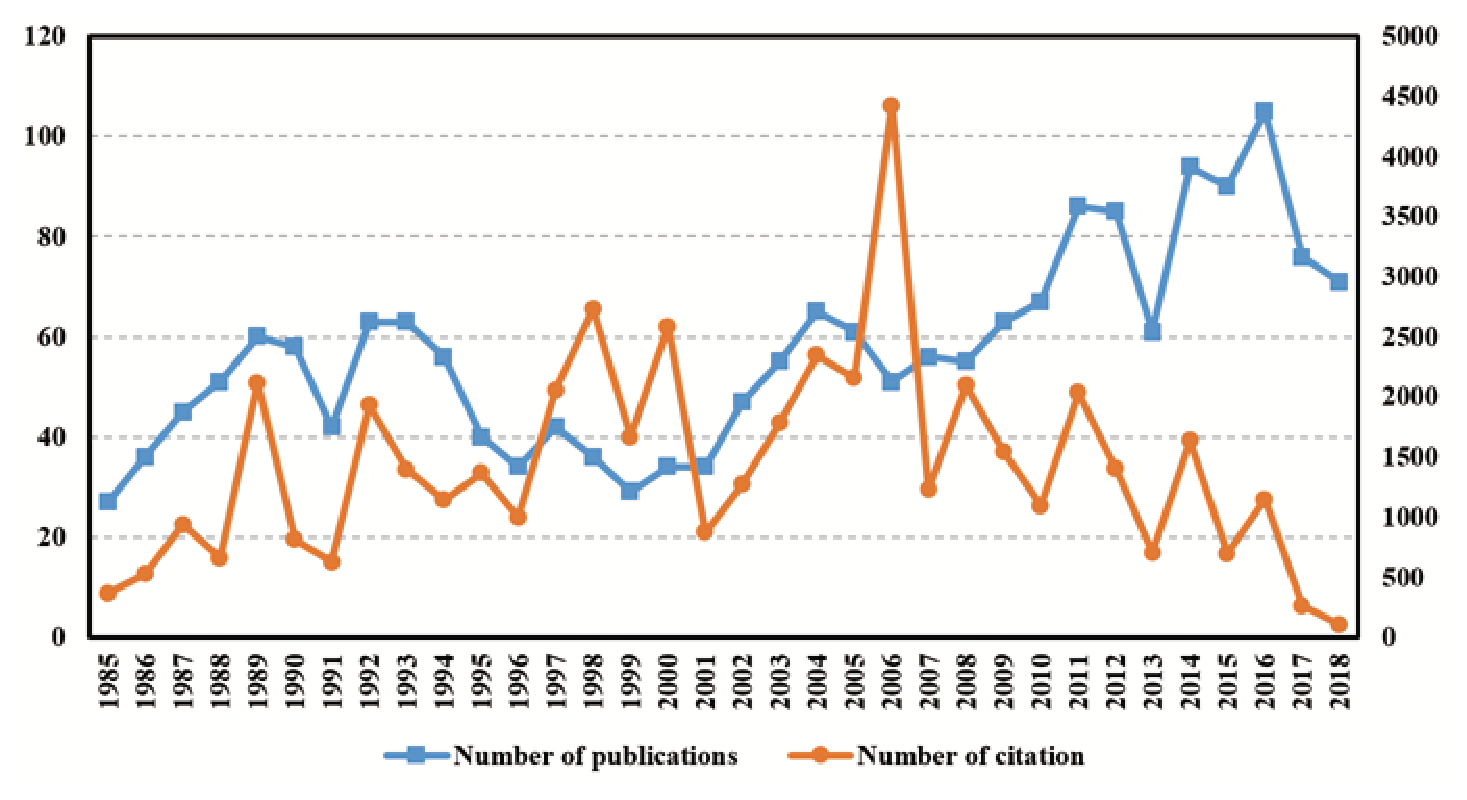
\includegraphics[width=\textwidth]{fig.1.eps}
\caption{Annual evolutions of IJF papers and citations from 1985 to 2018}
\end{figure}

\subsection{Citation network and co-citation
network}\label{citation-network-and-co-citation-network}

After an overall review about the total IJF papers from 1985 to 2018, we
focus on evaluating the performance of single IJF paper. The top 20 most
cited IJF papers are listed in table 1 with the information about the
citation number, author names, publication year, etc. Note that the
country in table 1 refers to the country of first author and UK contains
England, Scotland, Walsh, and North Ireland. TC, Nau, Nin refer to the
number of citations the paper received, the number of authors that the
paper has, the number of institutions that the paper belongs to,
respectively. The top three most cited papers all receive over 1000
citations, and the first one even possesses over 2000 citations. These
three papers already appear in the subsection 2.1 as the important
contributors for promoting the citations of their publication years. The
first one is the paper written by Zhang, Patuwo, and Hu (1998) which
investigated the research on forecasting with artificial neural
networks. The second is the work of Hyndman and Koehler (2006) which
considered the mean absolute scaled error as the standard measure based
on comparing the accuracy of multiple forecasting methods. The third is
Clemen (1989) which provided a review about the research on forecast
combination and suggestions for the future work.

\tablea

Besides, a citation network is mapped based on the citation relationship
between IJF papers. The citation network consists of nodes and links,
where some nodes are connected with links and some are isolated. A node
represents a paper and a link represents the citation relationship
between any two connected papers. The size of node is denoted as the
number of citations a paper received. Through this citation network, the
citation relationships between any connected IJF papers can be visually
obtained and deeper investigations like highly cited publications are
cited by what papers can be conducted easily. The number of citations no
less than 80 is set as the limitation, then 111 qualified IJF papers are
derived. 29 of the 111 papers are discarded because they are isolated.
Finally, 82 IJF papers are used to construct this citation map, as shown
in Fig. 2. Distance between any pair of papers denotes their similarity
calculated by the association strength method (Eck and Waltman 2009) The
longer distance is the more dissimilar the two connected papers are.
Papers with high similarity values are clustered and represented as the
same color. Among the 82 IJF papers, 70 of them have citations, while
the remaining 12 papers have no citations, but cite to some of the 70
papers. From Fig. 2, Zhang, Patuwo, and Hu (1998) is the biggest node
because it is the most cited paper among the total IJF papers, but among
these 82 IJF papers, it is not the paper that has the most citations
from the 82 IJF papers. The 82 IJF papers in Fig. 2 are all highly cited
papers, so their endorsements are pretty authoritative. Winning an
endorsement from these 82 papers helps a lot to promote the prestige of
the paper, so a further investigation is conducted to derive the highly
cited papers, where their citations are from these 82 papers. We define
the citation from the IJF papers as the local citation (LC). The papers
having no less than 5 local citations are extracted, as shown in table
2. Paper written by Gooijer and Hyndman (2006) is the most cited among
these 82 IJF papers, and the paper is about a 25 review on time series
forecasting based on the papers of JIF and Journal of Forecasting (JF).
According to the local citation percentage (LC/TC), the research of
Crone, Hibon, and Nikolopoulos (2011) ranks the first, which indicates
the high quality of its citations. Zhang, Patuwo, and Hu (1998) is top
one highly cited in the total IJF papers, but its performance in local
citation percentage is not that remarkable.

\tableb

\begin{figure}[htbp]
\centering
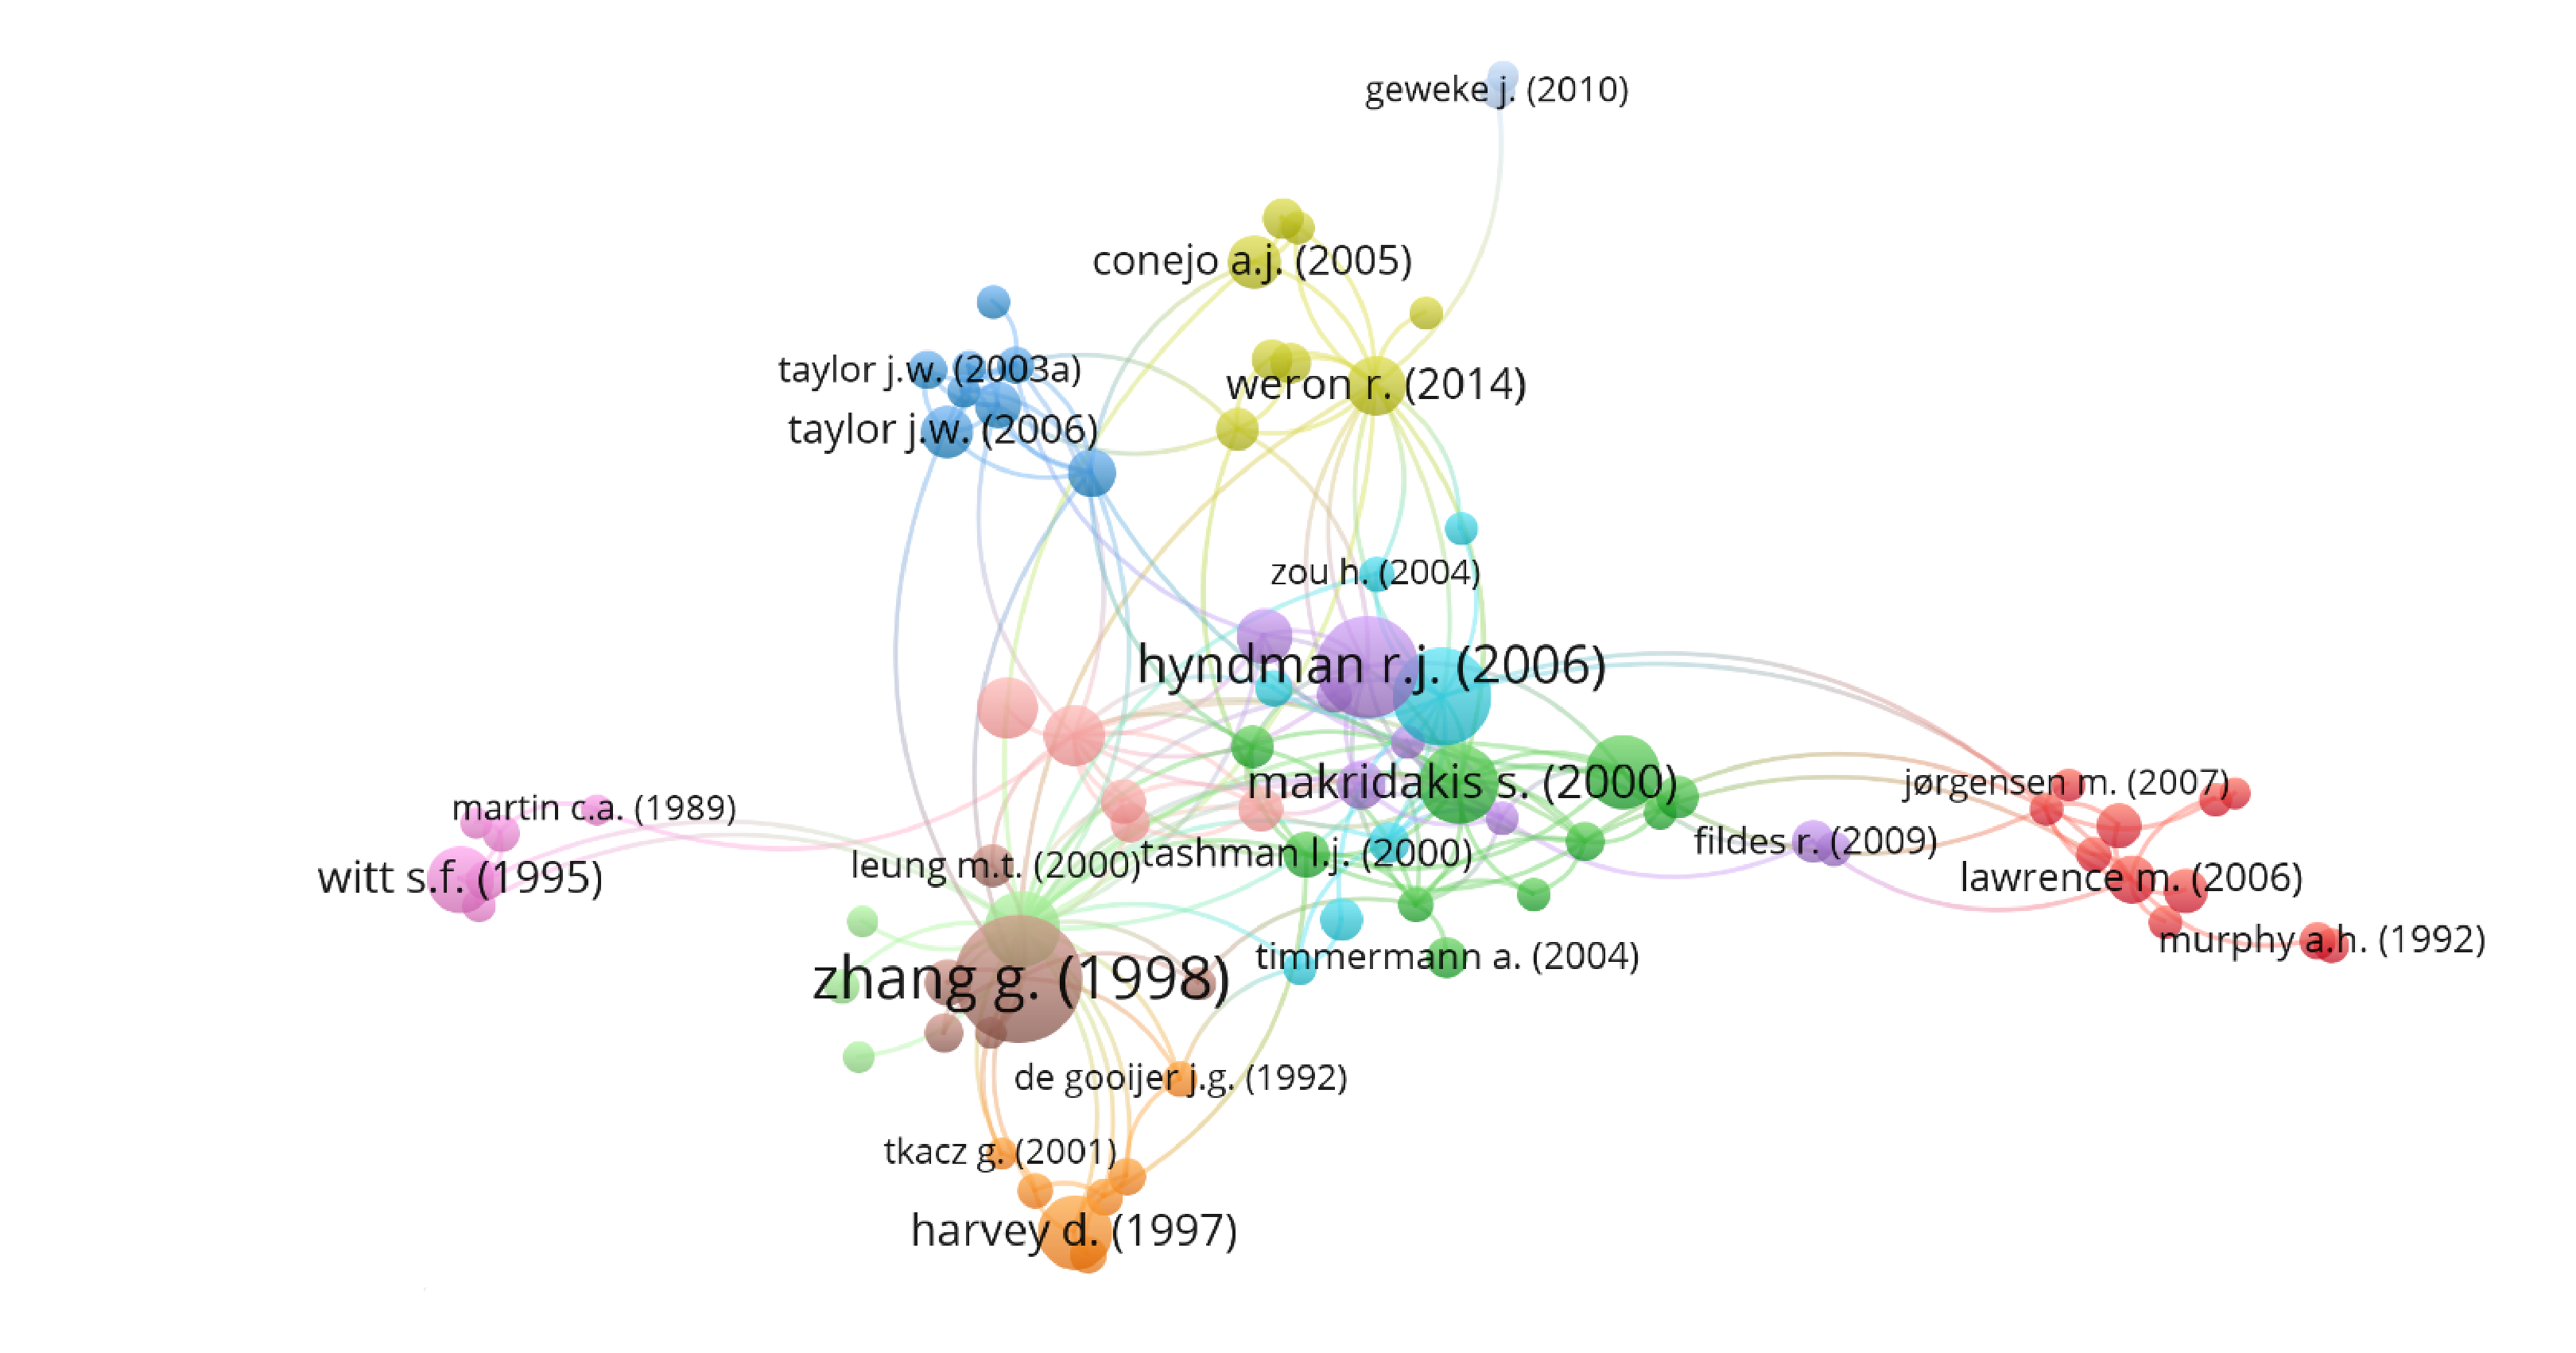
\includegraphics[width=\textwidth]{fig.2.eps}
\caption{Citation network of 82 most cited IJF papers}
\end{figure}

Co-citation analysis is one of the useful bibliometric methods. As the
name suggested, the co-citation relationship describes the relations
between any two co-cited papers, and the co-cited papers means papers
that are cited by the same paper. If two papers are cited by one same
paper, then these two papers are in a co-citation relationship and the
co-citation strength they possess is one. Based on the IJF papers
harvested from Scopus, the co-citation relationships between them and
citing papers are extracted. Note that 122 IJF papers are excluded
because of the missing data and format errors. Finally, 1816 IJF papers
and 33204 references are included in this co-citation network, shown in
Fig. 3. IJF papers published in the same year are divided into one group
to better straighten out their co-citation evolution trajectory.
Moreover, three groups of thresholding are used to control the
filtration of the qualified papers. Each group of thresholding has three
criterion which are the minimum citations, minimum co-citations, and
minimum normalized co-citations. The first thresholding is set in the
year of 1985, the second in 2002, and the last is in 2018. After some
trail runs, the first thresholding is set with 50, 3, 15, the second is
3, 3, 20, and the third is 3, 3, 20.

The color in the Fig. 3 denotes the publication year of papers, and the
warm color represents the latest year, while the cold color represents
the old year. The size of node denotes the co-cited times of each paper,
and the bigger the size is the more the co-cited times are. From Fig. 3,
we can see that the coldest color is green (i.e., approximately
corresponds to the year of 1998), which means the papers published
earlier are excluded according to the thresholding. The top 10 most
co-cited papers which have the biggest nodes are extracted and listed in
table 3. The most co-cited research conducted by Timmermann (2006)
elaborated on the advantages of forecast combination, and analyzed the
factors that can determine the advantages. The second most co-cited work
(Giannone, Reichlin, and Small 2008) provided a framework which was
useful for the real-time forecast selection based on conditional
expectations of forecasts, and applied this framework into a testing
problem. The third most co-cited work is an IJF paper written by
Makridakis and Hibon (2000) which described a M3-Competition. This IJF
paper also is the main contributor for the high citations in the year of
2000. Including the work of Makridakis and Hibon (2000), we find that
four of the ten most co-cited papers are IJF papers, which means these
four IJF papers possess the most co-endorsements from IJF papers.

In table 3, except for the co-citation (Co), the information about the
first co-cited year (FY), the last co-cited year (LY), the whole
co-cited duration (Y), and the average co-citation per year (Ave-Co)
about each top ten co-cited papers are provided. In table 3, we use the
abbreviations of journals, which are Handbook of economic forecasting
(HEF), International Journal of Forecasting (IJF), Journal of Monetary
Economics (JME), Principles of Forecasting: A Handbook for Researchers
and Practitioners (PF: AHRP), and Journal of the American College of
Cardiology (JACC). Among these four IJF papers, we find the research
conducted by Hong et al. (2016) has the shortest co-cited duration, but
the highest average co-citation per year, which denotes the research
(Hong et al. 2016) is very frequently co-cited by others in recent
years. From the Fig. 3, we can see the study (Hong et al. 2016) is in a
co-citation relationship with his another research (Hong, Pinson, and
Fan 2014), and these two researches are both related to the energy
forecasting. Another two IJF papers are the work of Hyndman and Koehler
(2006) and the work of Fildes et al. (2009) which both possess
relatively low average co-citation per year, and it denotes they are
behind Hong's work (Hong et al. 2016) in co-cited activity. One thing is
interesting that the node of Fildes et al. (2009) is wrapped with a
purple ring in Fig. 3, where the purple ring means the node enjoys a
high between-ness centrality. The between-ness was proposed by Freeman
(1977) and depicts the structural property of communication of nodes
between connected networks. A node with high between-ness centrality
denotes it is more inclined to be positioned between some connected
networks. In Fig. 3, the node of Fildes et al. (2009) is between a red
cluster and a yellow cluster, which means the node of Fildes et al.
(2009) linked the researches published earlier than 2009 and later than
2009. Fildes et al. (2009) plays an important role in expressing the
connected co-citation relationships between these two clusters of
researches. Besides, another work called burst detection is conducted to
identify papers with abrupt change (Kleinberg 2003), as shown in table
4. The papers with abrupt change usually are the milestone papers of the
science mapping research. From Fig. 4, we can find that the same four
IJF papers having high co-citations are also remarkable in this burst
detection, especially, the work of Makridakis (Makridakis and Hibon
2000) has the strongest burst power, which means it is the most
important milestone in this co-citation mapping.

\begin{figure}[htbp]
\centering
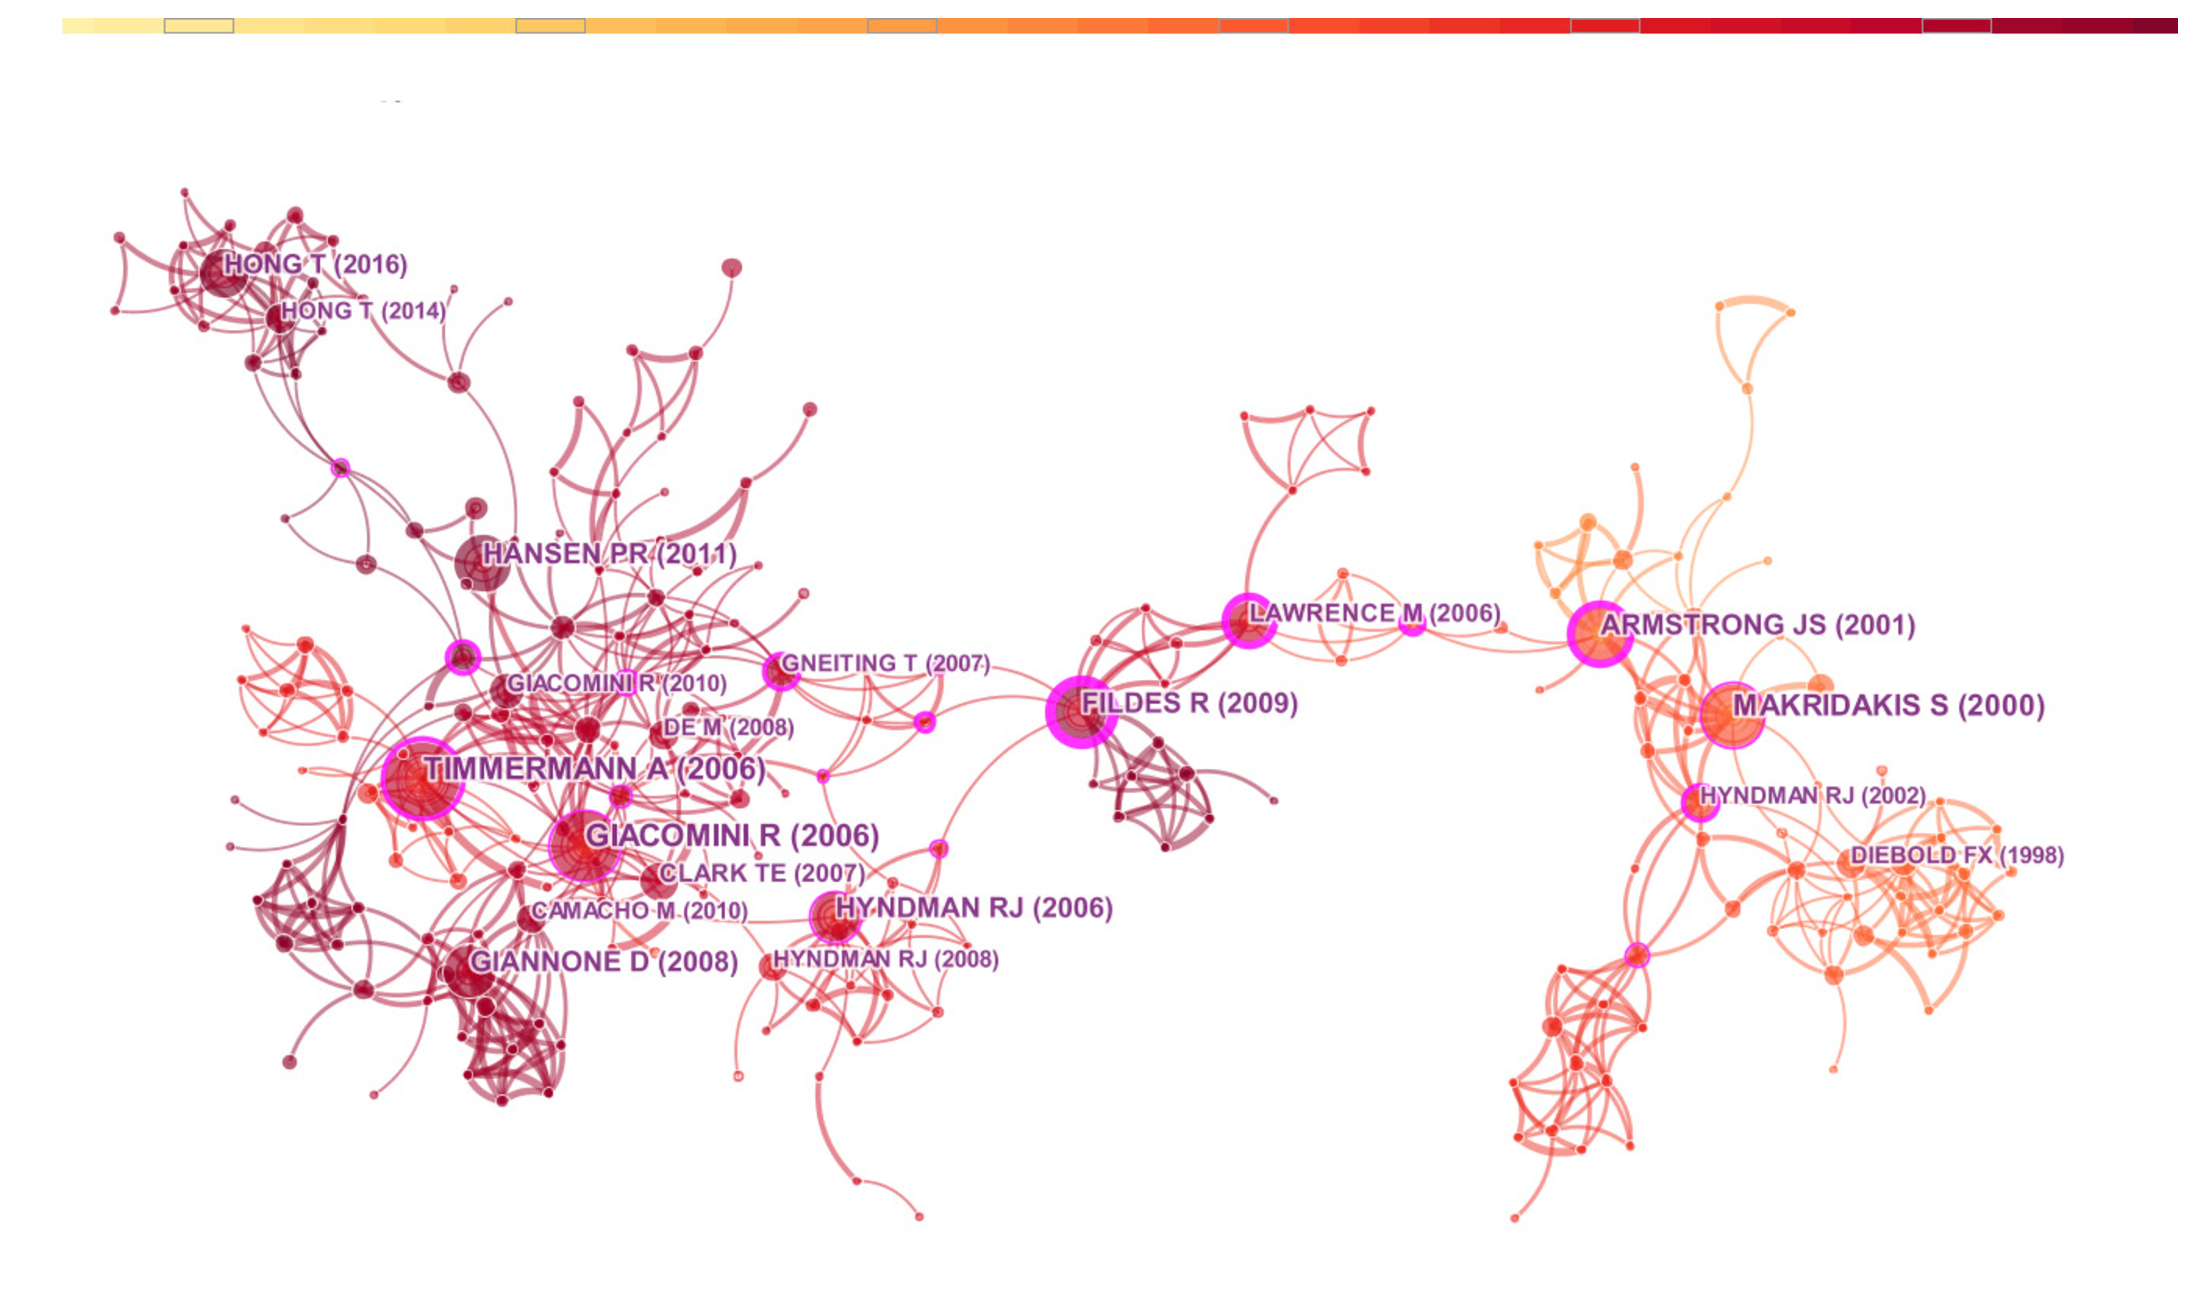
\includegraphics[width=\textwidth]{fig.3.eps}
\caption{Co-citation network of IJF papers and their citing papers}
\end{figure}

\newpage

\tablec

\tablezzzzz

\subsection{Authors analysis in IJF and co-author
network}\label{authors-analysis-in-ijf-and-co-author-network}

Prolific authors can be regarded as the experts of the field or the
important contributors of the journal. After a preliminary review, some
prolific associate editors who published in IJF are excluded because the
researches of associate editors are more inclined to be highly cited
than those of normal IJF authors. The top ten prolific authors in IJF
are selected from the remaining IJF authors, as shown in table 5. The
information about their first paper year, and last paper year is stated
in table 5. We find that most of the ten prolific authors possess a long
academic career, especially Koehler and Ord whose papers covering at
least 30 years. Five of the ten authors affiliated in USA, which
indicates the USA scholars form a leading and active community in IJF.
Generally speaking, first author is the main contributor of a paper, and
corresponding author is responsible for a paper. Therefore, we calculate
the number of papers that the authors are responsible for the first
authors or the corresponding authors. Four indicators are used: 1st (the
number of papers that are first-authored), 1st \% (1st/TP), Cor (the
number of papers that are corresponding-authored), and Cor \% (Cor/TP).
From table 4, Chatfield's first author percentage is 86.67\% which is
the highest among the ten authors, followed by Taylor and Lahiri.
O'Connor and Ord are two authors who have relatively weak performance in
first author percentage and corresponding author percentage. It means
that they are prolific authors in IJF, but in most cases, they acted as
a collaborator of the papers, rather than the main contributor.

\tabled

The number of citations an author received is a useful indicator to
evaluate the prestige of authors, therefore, the top ten most cited
authors are selected in table 6. Similar to the table 5, the associate
editors are excluded in table 6. Koehler is the most cited author due to
his relatively high output. Wright has the highest TC/TP value, which is
largely due to his highly cited paper, ``The Delphi technique as a
forecasting tool: Issues and analysis'' (Rowe and Wright 1999). Franses
is the most prolific author, but ranks the last in TC, which indicates
his researches are not as attractive as those of the other nine authors.
Besides, the number of citations from the IJF and outside the IJF are
calculated. Goodwin, Collopy, Hibon and O'Connor receive higher local
citation percentage, which means the IJF endorsements their researches
obtained are more than those of the remaining authors.

\tablee

A co-author network is constructed based on the co-author relationship
between IJF authors. Authors who publish less than eight papers are
discarded, then 38 qualified authors are derived. Among the 38 authors,
6 authors are isolated, so finally 32 authors are mapped into the
co-author network, as shown in Fig.4.

\begin{figure}[htbp]
\centering
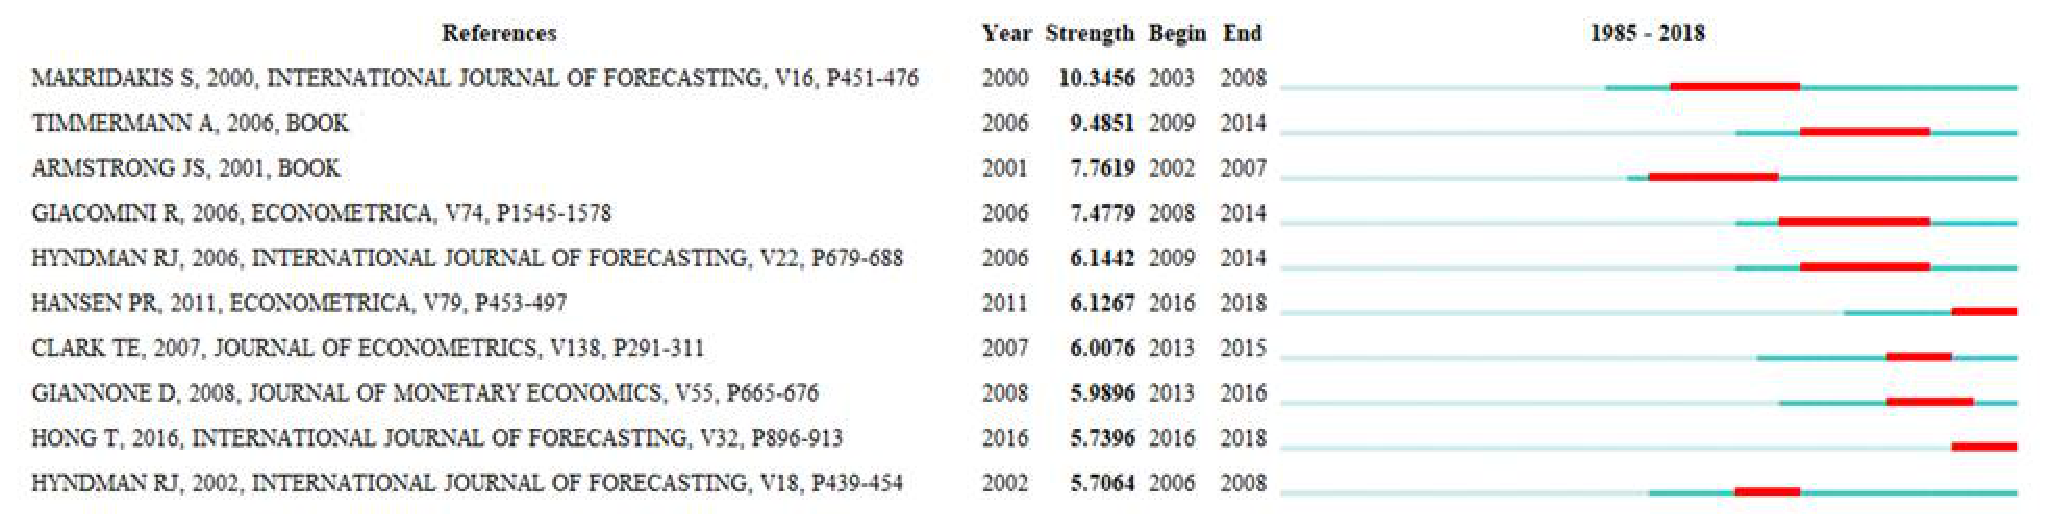
\includegraphics[scale=0.35]{fig.4.eps}
\caption{Co-author network of the most prolific IJF authors}
\end{figure}

\subsection{Country analysis and country co-occurrence
network}\label{country-analysis-and-country-co-occurrence-network}

In this subsection, we extract some prolific countries and most
attractive countries according to the number of publications and
citations. Based on this analysis, we can identify what countries are
the biggest providers of IJF and what countries possess the highest
authority in IJF. Besides, a country co-occurrence network is provided
to express the collaboration relationships among different countries.

Country is a geographical community producing the academic researches,
and the large academic output of a country declares the high academic
productivity of the country. Therefore, country is selected as the
objective of this subsection, and analyzed based on the number of papers
each country produced and the number of citations they received.
Information about the top ten prolific countries are listed in table 7.
USA, UK, and Australia rank the top places, and their durations range
the whole issue period of IJF. USA is the dominant country whose papers
occupy around 41\% of the total IJF papers. Moreover, most of the
prolific countries belong to Europe and North America, which indicates
the developed countries in Europe and North America are still the main
producers of IJF papers.

\tablef

Besides, a dynamic analysis is conducted based on the output of top
three countries which are USA, UK, and Australia, as shown in Fig. 5.
Two indicators are used: percent 1 (the ratio of the yearly IJF papers
produced by certain country to the yearly number of total IJF papers),
and percent 2 (the ratio of the yearly IJF papers produced by certain
country to the total number of IJF papers produced by certain country).
Observing from the percent 1, although USA is in a leading position, its
dominance has been gradually weakened from 1985 to 2018. However, the
values of percent 1 of UK and Australia keep on increasing from 1985 to
2018. From the percent 2, the values of USA is relatively stable, but
with a short-time drop during 1995 to 2001. The values of UK and
Australia are increasing overall. The value of percent 2 of Australia in
2016 have an obvious peak. In the IJF papers produced by Australia, the
number in 2016 occupies 9.55\% of the number in total.

The number of citations a country possesses is an important indicator to
evaluate the prestige of it, and also is a sign of knowledge spreading
from the country. Therefore, the top ten most cited countries are
selected in table 8. USA is the most highly cited country, and its
citations are nearly double of the UK' citations. Compared to the table
6, Belgium drops out of the list of top ten most cited countries, and
Turkey replaces Belgium as the member of top most cited countries.
Except for the number of citations, the number of citations per paper is
provided, and it reveals the attraction of single paper. One thing is
interesting that USA dominates the advantage in the total number of
citations, but it is behind Australia, France, Turkey and UK in the
number of citations per paper. What is more, we calculate the number of
citations from the IJF (In-TC) and the number of citations outside the
IJF (Out-TC). The former demonstrates how many IJF researches pay
attention to the papers of the country, and the latter shows the
prestige that the papers of the country possesses outside the IJF. USA
is the most prolific country, but its citation percentage from the IJF
is the lowest, which means its researches caught more attention from
journals outside the IJF. On the contrary, Italy, France, and Germany
possess a relatively high citation percentage from the IJF, which means
these countries receive more endorsements from the researches in IJF
compared with the remaining countries.

\newpage

\begin{figure}[!htbp]
\centering
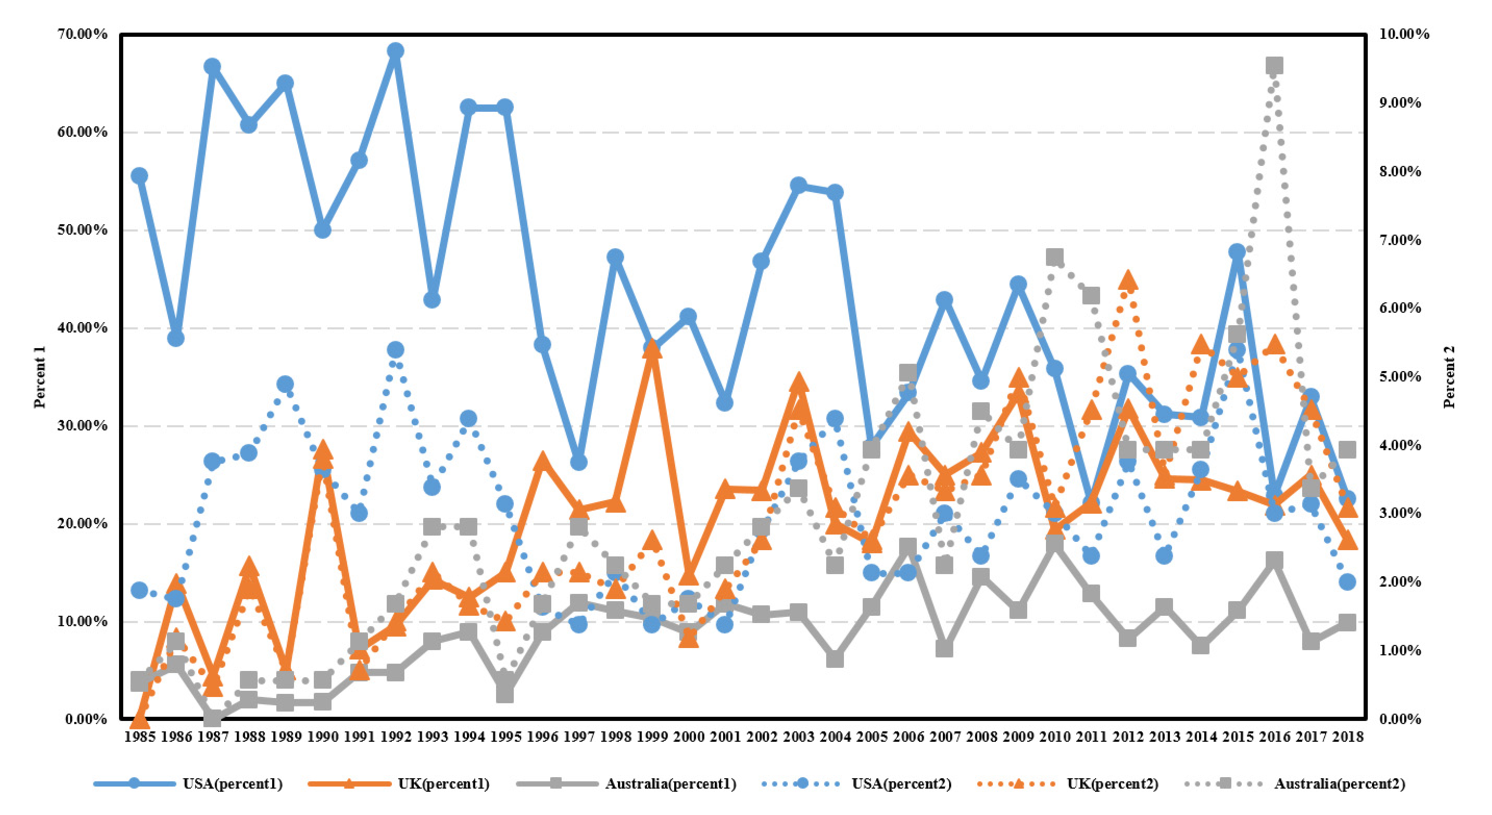
\includegraphics[width=\textwidth]{fig.5.eps}
\caption{The dynamic of the academic productivity of the prolific countries}
\end{figure}

\tableg

What is more, a country collaboration network is mapped in Fig. 6. The
size of label denotes the number of papers a country produced, and the
links between any connected labels indicates the collaboration
relationships between connected countries. 25 countries that published
no less 15 times are extracted to construct the country collaboration
network. The detailed information including Link (the collaboration
times a country possesses), CM (the country that collaborate most with
the target country), Number (the collaboration times that CM
collaborates with the target country) and N/L (the percentage that
divides Number by Link) is stated in table 8. USA ranks the first in
table 8 with 217 collaboration times, followed by UK with 201
collaboration times. Moreover, USA and UK are the countries that
cooperate with each other the most. Besides, 11 countries cooperate with
USA the most, and 9 countries cooperate with UK the most. Australia
ranks the third in table 9, but it is not the most collaborated country
to any of the countries in table 8, while Netherlands is the most
collaborated country to Belgium, Denmark, and Austria.

\begin{figure}[htbp]
\centering
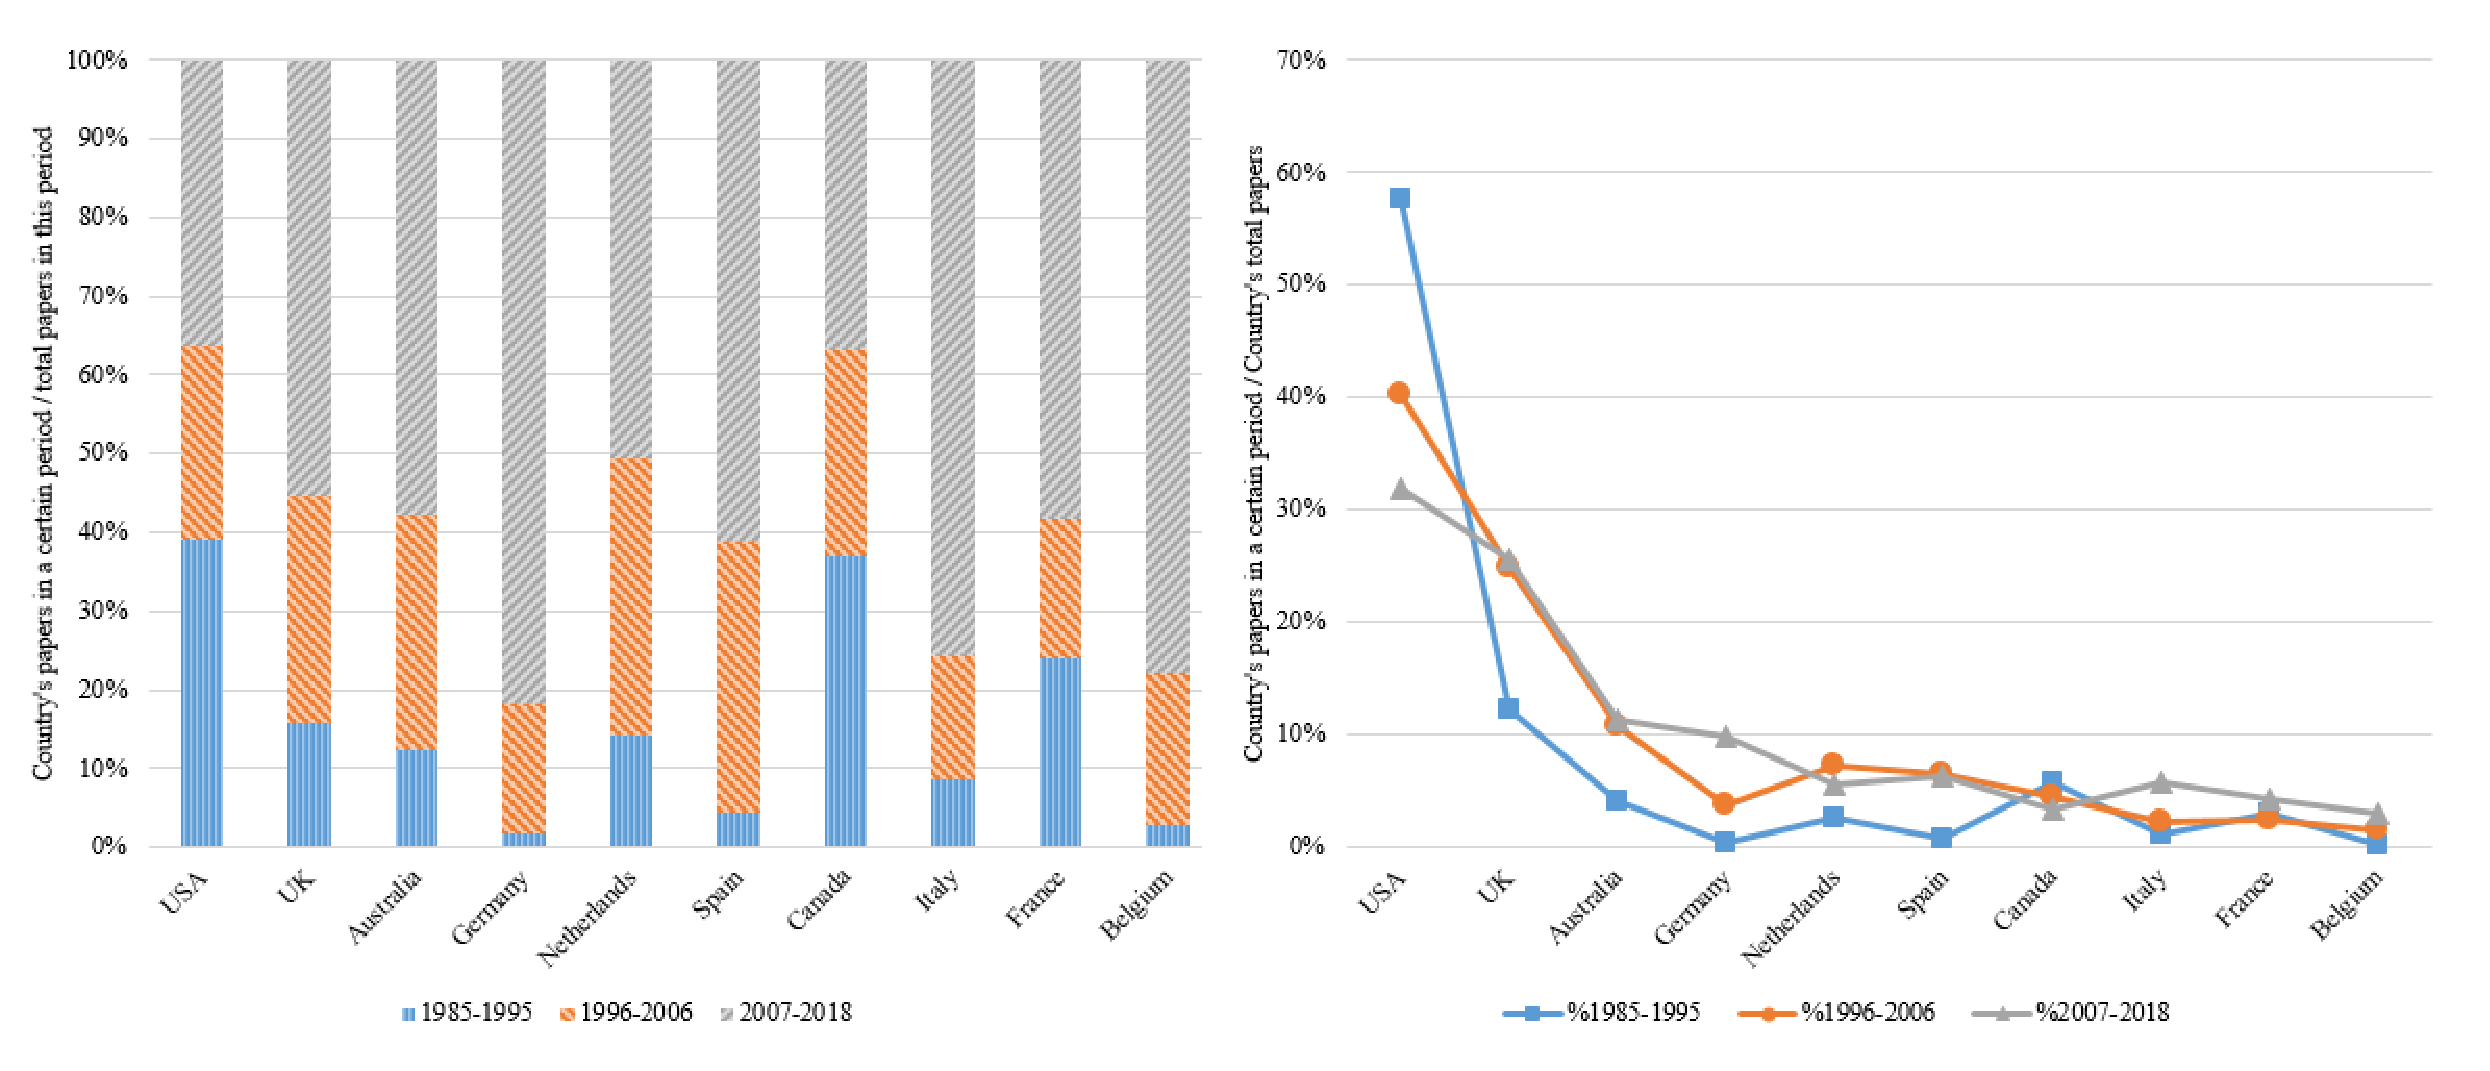
\includegraphics[scale=0.5]{fig.6.eps}
\caption{Country collaboration network}
\end{figure}

\tableh

\section{Knowledge diffusion analysis of the forecasting
journals}\label{knowledge-diffusion-analysis-of-the-forecasting-journals}

In academics, knowledge diffuses along with the citing behaviors of
papers, and papers belong to different subject areas according to their
research contents. In Scopus, subject areas are usually considered as
the labels to classify the different kinds of knowledge. In this study,
subject areas are used for conducting the knowledge diffusion analysis.
However, categorizations on subject areas exist deviations because of
the informal acquisition (Leydesdorff and Goldstone 2014), therefore,
the analysis only relying on the level of subject areas is easily to be
subject to a biased result. For this reason, the knowledge diffusion
analysis is conducted both at the subject area level and the journal
level.

As one of the leading forecasting journal, IJF was launched in 1985
following another authoritative forecasting journal, Journal of
Forecasting (JF). These two leading forecasting journals are the
important members in the International Institute of Forecasting (IIF).
Therefore, in this study, in order to have a broader overview about the
knowledge fertilization in the forecasting field, both of IJF and JF are
included in the knowledge diffusion analysis.

\subsection{Analysis at the level of subject
area}\label{analysis-at-the-level-of-subject-area}

In this subsection, papers cited IJF and JF papers are selected,
respectively, as the raw data. A static analysis about the subject area
distribution is provided to figure out which subject areas pay attention
to the forecasting papers. Moreover, a dynamic analysis is supplemented
to describe how the subject area distribution evolves over time.
Forecasting papers in different periods may attract researches from
different subject areas.

In Scopus, IJF papers ranging from 1985 to 2018 was retrieved, and then
29464 citing papers ranging from 1985 to 2019 were harvested. Similarly,
16419 citing papers are obtained based on JF papers from 1982 to 2018.
The top ten most prolific subject areas among the citing papers are
stated in table 10. Four indicators are used: the number of citations
that the IJF papers belonging to the subject area received (NP1),
NP1/29464 citing papers of IJF (Percent1), the number of citations that
the JF papers belonging to the subject area received (NP2), and
NP2/16419 citing papers of IJF (Percent2). We find that IJF citing
papers and JF citing papers possess the same prolific subject areas,
which denotes both of the journals have very similar audiences. IJF and
JF were set with an aim that become an output for the BEM forecasting
researches (Fildes 2006). From the angle of knowledge diffusion, this
aim has been successfully achieved because Computer Science, Economics,
Econometrics and Finance, and Business, Management and Accounting have
become the three dominant subject areas based on the forecasting citing
papers.

\tablei

\subsection{Analysis at the level of
journal}\label{analysis-at-the-level-of-journal}

Based on the subsection 3.1, the knowledge flow analysis at the level of
subject area has been completed, but the scope of subject area is kind
of wide-ranging. Therefore, the research scope is narrowed to the level
of journal to conduct a further knowledge flow analysis. The subject
areas which have a special performance in subsection 3.1 will be
analyzed as the primary research objectives, and the citation
relationships between different journals within the same subject area
will be elaborated and visualized in citation networks. Moreover, all of
the analysis is dynamic to better elaborate the evolution progress of
the knowledge flow among the different journals. Considering the
authority of IJF and JF in the forecasting field, the knowledge
diffusion processes starting from IJF and JF are both delineated based
on their citations relationships. The forecasting-related applications
published in the journals outside the forecasting journals are
investigated. Note that only the top three subject areas in IJF and JF
respectively are elaborated in the following content, only we only
display the journal citation networks of the top three subject areas.
The remaining seven subject areas in IJF and JF and their journal
citation networks are given in the Appendix.

\subsubsection{Knowledge diffusion within the same subject area starts
from
IJF}\label{knowledge-diffusion-within-the-same-subject-area-starts-from-ijf}

Knowledge diffusion starts from IJF has been investigated in 3.1.2, and
the top three subject areas are Computer Science, Economics,
Econometrics and Finance, and Business, Management and Accounting. All
of the citing papers belonging to these three subject areas are
harvested, respectively, then aggregate them into the level of journal,
and the journal citation relationships between different journals within
the same subject area are extracted and mapped in journal citation
networks. Four parameters are used to evaluate the journal citation
network, including clusters (the number of groups containing the same
color nodes), local links (the number of links), link strength (the
total strength that each link possesses), and items (the number of
nodes). Note that the size of node in the network represents the number
of publications that the journal published, and the thickness of link
between connected nodes represents the number of citations between the
connected journals.

\noindent 3.2.1.1. Journal citation network in Computer Science

All the citing papers belonging to Computer Science are harvested. 21
Journals that have no less than 50 publications and 700 citations are
selected to map the IJF journal citation network in Fig. 7, and the
journal citation structure can be intuitively observed from Fig. 7. 21
Journals that have no less than 40 publications and 200 citations are
selected. Four parameters are clusters (7), local links (169), link
strength (6146), and items (21). The top ten journals that have the most
citation connections in this journal citation network are extracted.
Note that the information about the top ten journals is stated in table
11.

\begin{figure}[htbp]
\centering
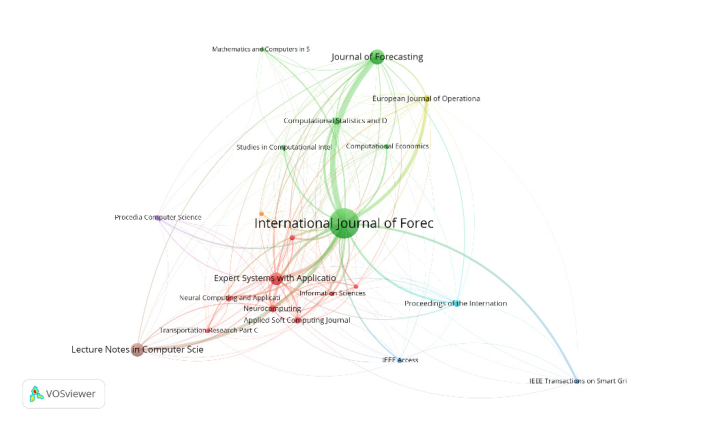
\includegraphics[width=\textwidth]{fig.7.eps}
\caption{IJF Journal citation network in Computer Science}
\end{figure}

Observing from the Fig. 7, IJF occupies a central place in network with
other journals around it. The link between IJF and JF is the thickest in
this journal citation network, which indicates JF has the most citation
connection with IJF. The node size of JF, Expert Systems with
Applications, and Lecture Notes in Computer Science is similar, which
indicates these three journals published a similar number of
publications within the range of IJF citing papers. However, the
thickness of the links which are between IJF and Expert Systems with
Applications as well as between IJF and Lecture Notes in Computer
Science is thinner than that of the link which is between IJF and JF. In
the table 11, two indicators are provided: Links (the number of
citations that journal has within selected IJF citing papers in Computer
Science), Links with IJF (the number of citations that are between the
journal and IJF), and \% (Links/ Links with IJF \%). JF, European
Journal of Operational Research, Computational Statistics and Data
Analysis, and Proceedings of The International Joint Conference on
Neural Networks have a high percentage, which demonstrates most of their
citations are related to IJF.

\tablej

\noindent 3.2.1.2. Journal citation network in Economics, Econometrics
and Finance

21 Journals that have no less than 35 publications and 400 citations are
selected to map the IJF journal citation network in Economics,
Econometrics and Finance. The journal citation relationships based on
the citing papers belonging to Economics, Econometrics and Finance are
depicted in the Fig. 8, and the detailed information is stated in table
12. From the structure of the network, IJF is a dominating center.
International Journal of Production Economics locates far from the other
journals in the journal network, and the links between International
Journal of Production Economics and related journals is much less than
that of other connected journals in the journal network. In the table
11, most journals have a percentage less 50\%, however, International
Journal of Production Economics has a very high percentage (i.e.,
95.27\%). We can find that 403 of the 423 citing papers of International
Journal of Production Economics are linked to IJF. Journal of Applied
Economics ranks third in the table 12, but only 350 citing papers are
linked to IJF.

\tablek

\newpage

\begin{figure}[htbp]
\centering
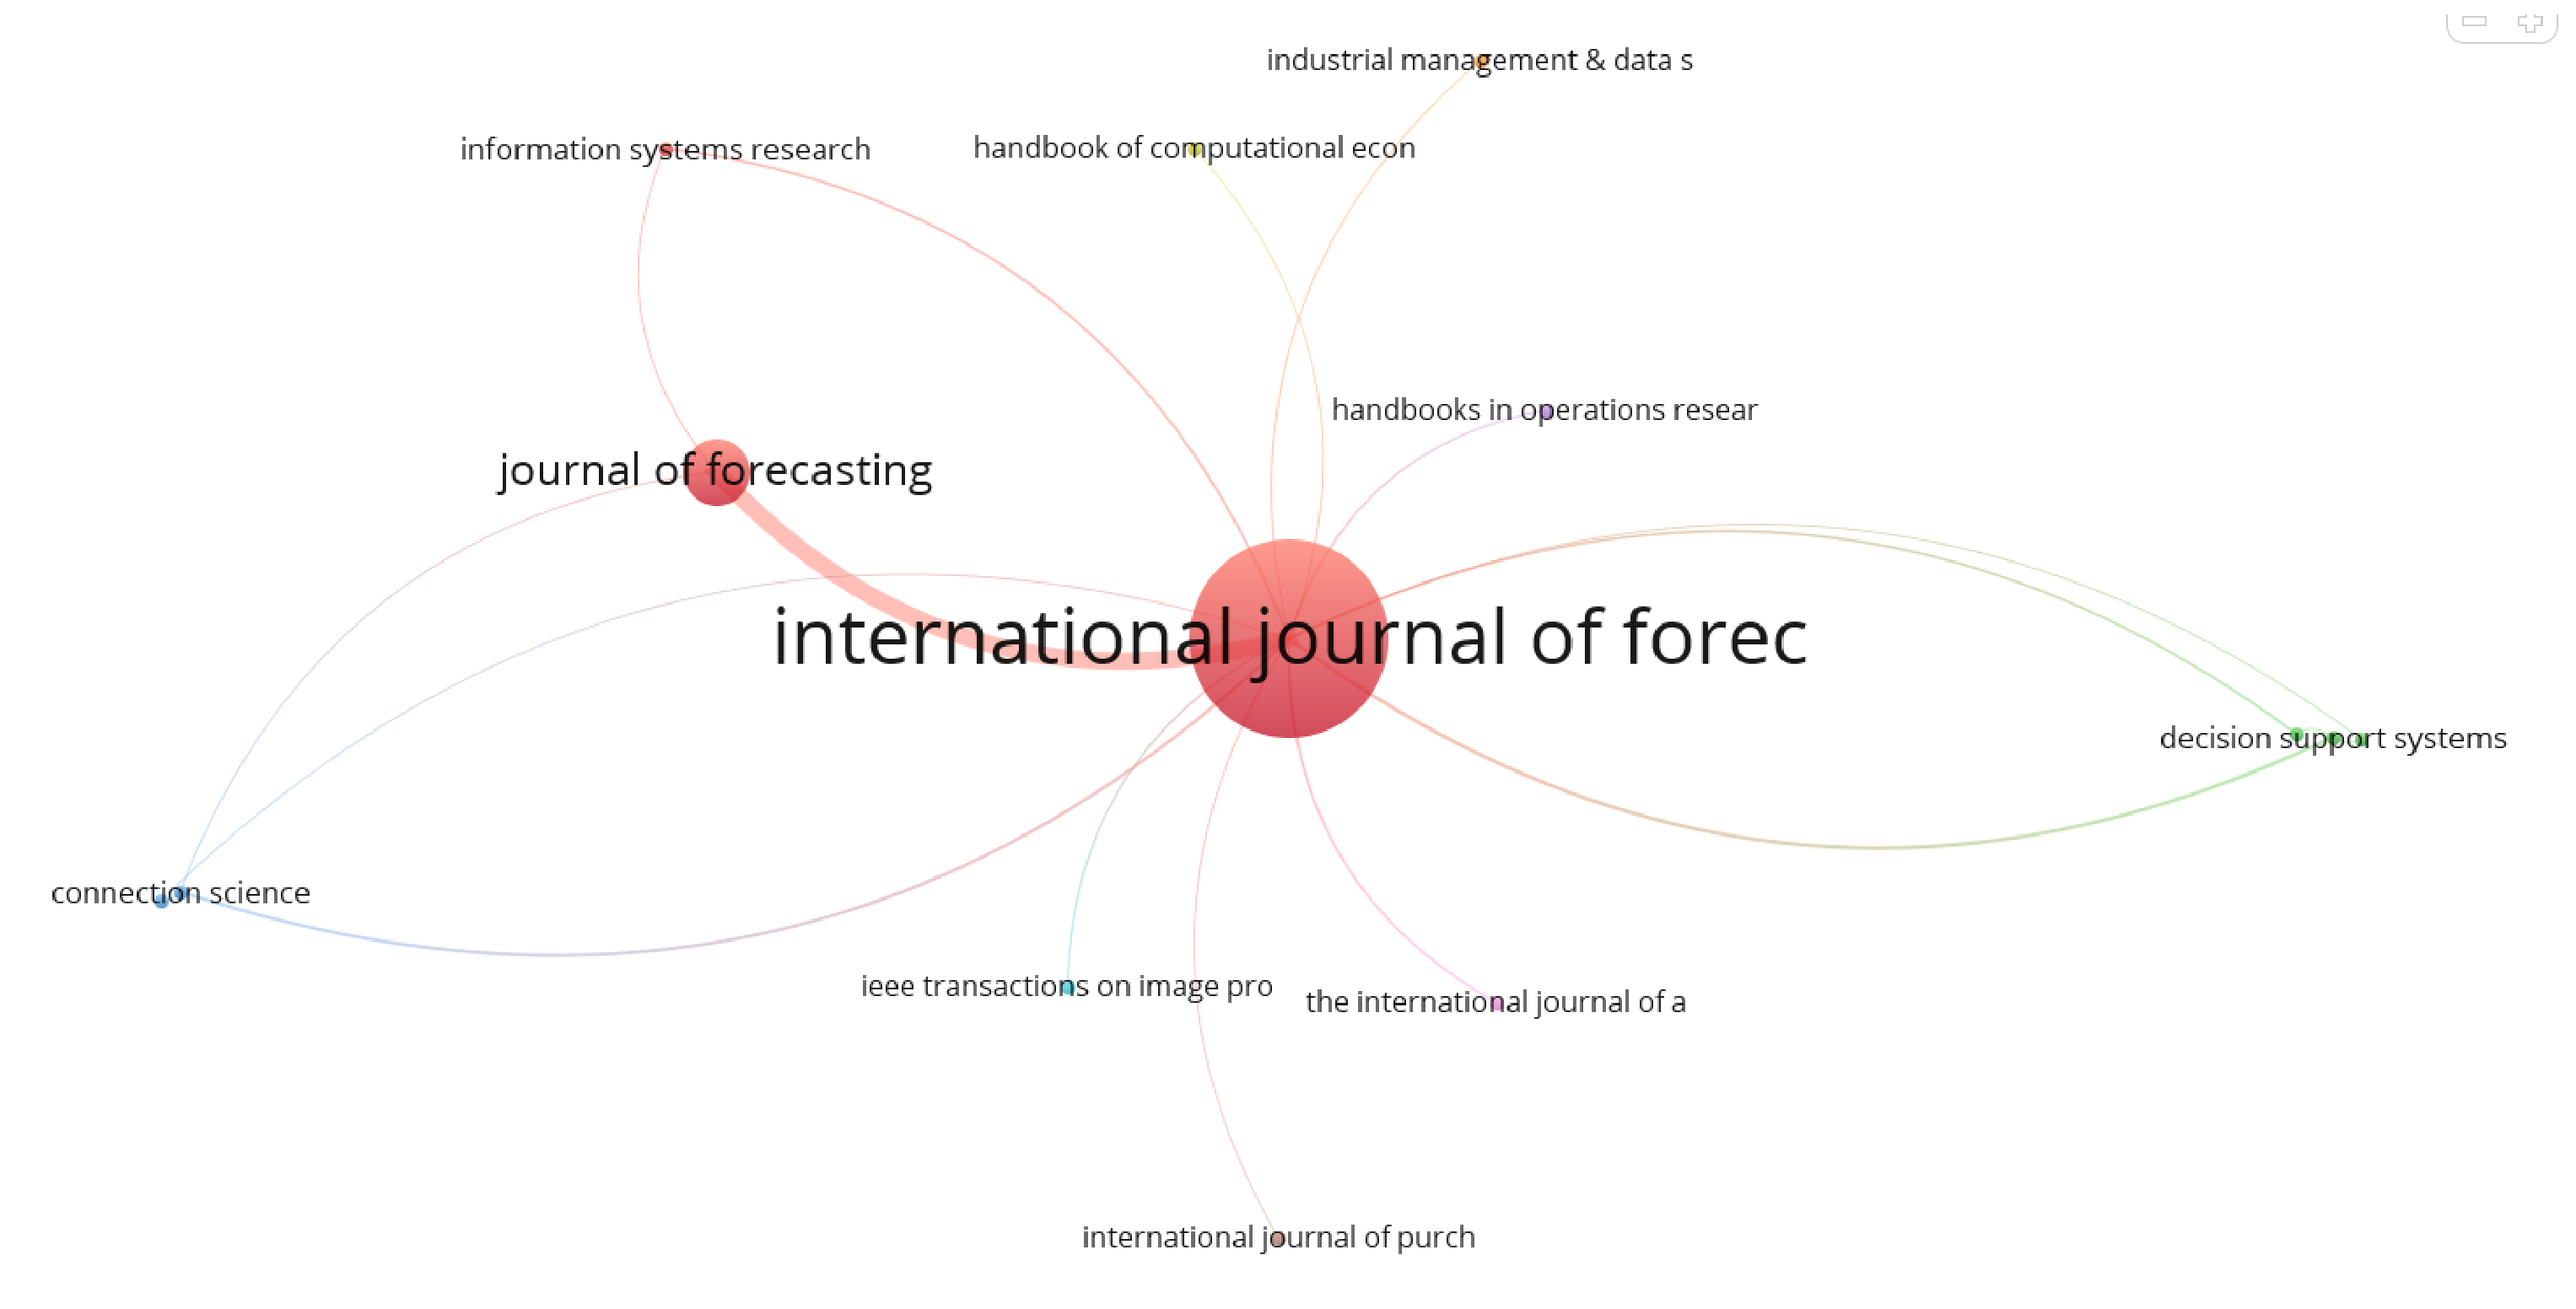
\includegraphics[width=\textwidth]{fig.8.eps}
\caption{IJF Journal citation network in Economics, Econometrics and Finance}
\end{figure}

\noindent 3.2.1.3. Journal citation network in Business, Management and
Accounting

21 Journals that have no less than 20 publications and 300 citations are
selected to map the IJF journal citation network in Business, Management
and Accounting. The journal citation relationships based on the IJF
papers and citing papers belonging to Business, Management and
Accounting are depicted in the Fig. 9, and the detailed information is
stated in table 13. From the Fig. 9, IJF is the absolute center in the
network, and JF is the most citing journal. Some Tourism-related
journals locate in the right of the network, which are far away from the
remaining journals. In the table 13, some journal have many papers
citing IJF papers, while others only have a few papers citing IJF
papers. JF (81.81\%) and Technological Forecasting and Social Change
(70.42\%) are two journals that have the highest percentages of citing
papers. Annals of Tourism Research (19.63\%), Tourism Management
(22.32\%), Journal of Travel Research (22.47\%), and Tourism Economics
(29.86\%) have the lowest percentages of citing papers, which are all
Tourism-related journals.

\tablel

\newpage

\begin{figure}[htbp]
\centering
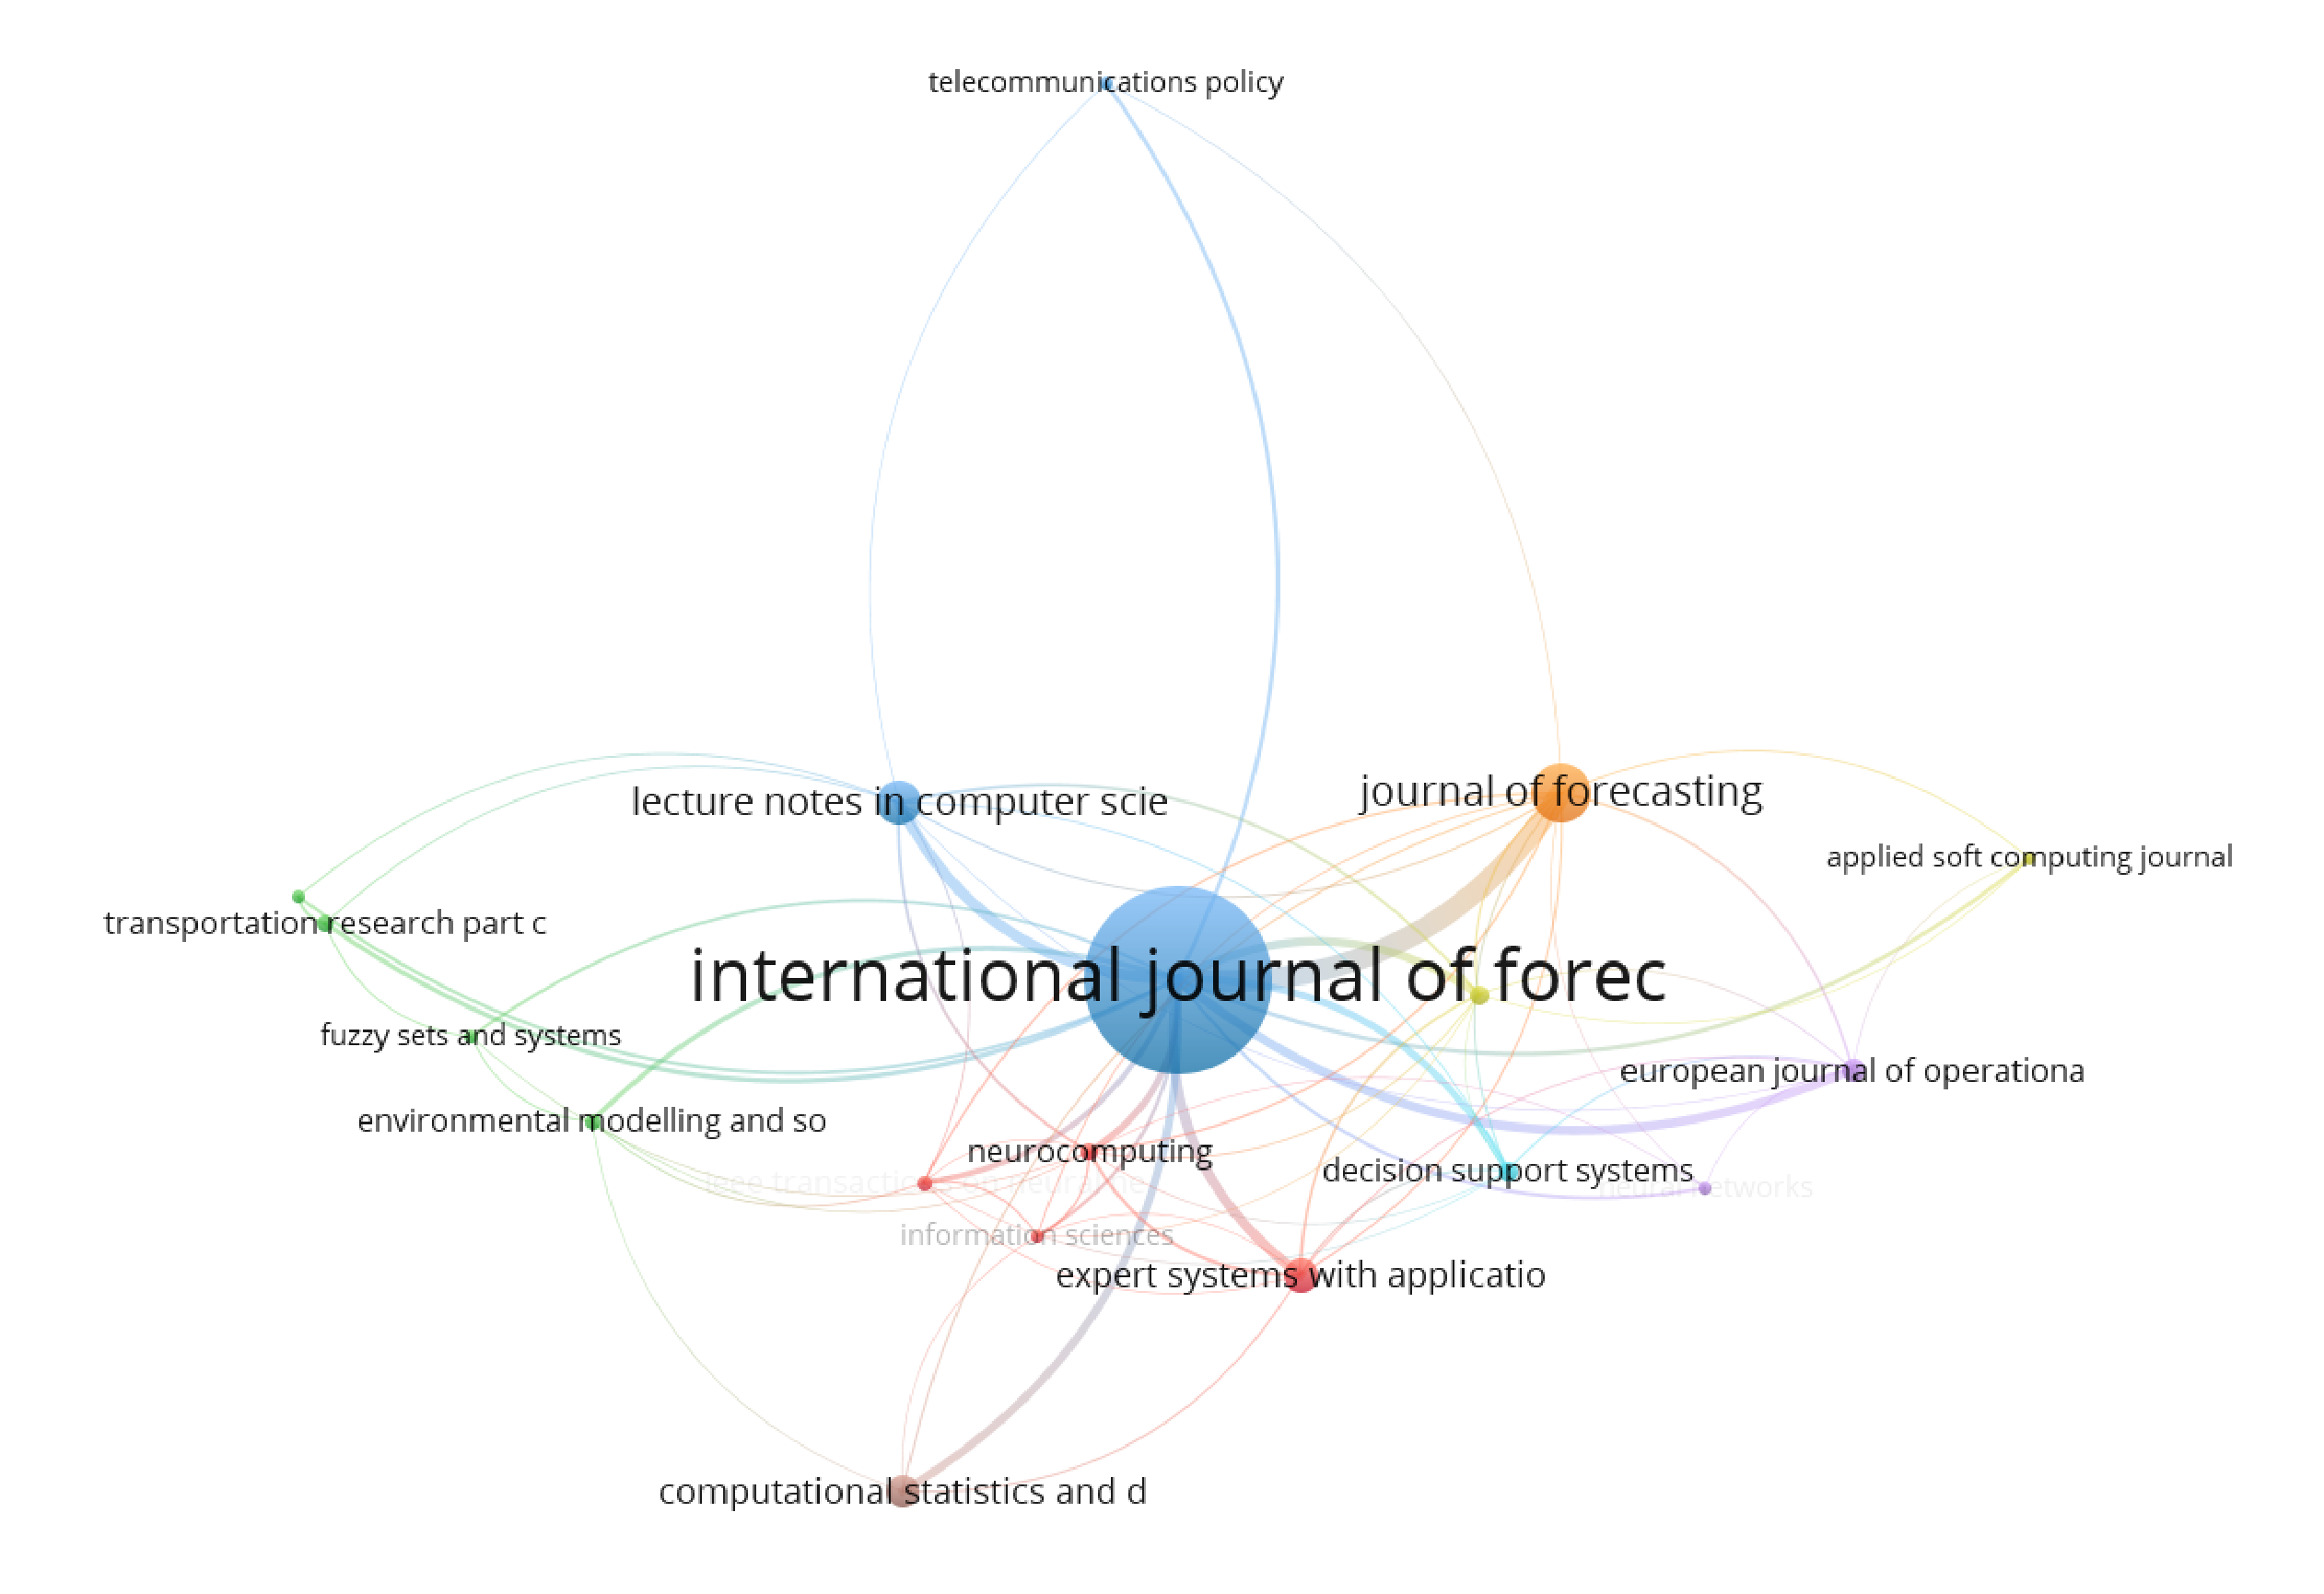
\includegraphics[width=\textwidth]{fig.9.eps}
\caption{IJF Journal citation network in Business, Management and Accounting}
\end{figure}

\subsubsection{Knowledge diffusion within the same subject area starts
from
JF}\label{knowledge-diffusion-within-the-same-subject-area-starts-from-jf}

Knowledge diffusion starts from JF has been investigated in 3.1.2, and
five subject areas have a special performance, which are Business,
Management and Accounting, Economics, and Mathematics. All of the citing
papers belonging to these five subject areas are harvested,
respectively, then are aggregate them into the level of journal, and the
journal citation relationships between different journals within the
same subject area are extracted and mapped in journal citation networks.
The citation connection between IJF and JF is very strong in the journal
citation networks of IJF, however, in the journal citation networks of
JF, their citation connection becomes much weaker, which denotes that
the knowledge diffusing strength starting from JF to IJF is weaker than
from IJF to JF.

\noindent 3.2.2.1. Journal citation network in Business, Management and
Accounting

21 Journals that have no less than 20 publications and 300 citations are
selected to map the JF journal citation network in Business, Management
and Accounting. JF papers and their citing papers belonging to Business,
Management and Accounting are selected and the journal citation network
is extracted in Fig. 10. The detailed information about the journal
network is stated in the table 14. In the Fig. 10, the link of JF and
IJF is the thickest in the journal network, which means IJF has the most
citations citing JF papers. Similar as the journal network of the
subsection 3.2.1.3, Tourism-related journals still exist in this journal
network of Fig. 10. From the table 14, these tourism-related journals
all have a lower percentage of citing papers. Except for IJF, the
remaining nine journals in the table 14 all have a percentage lower than
50\%.

\tablem

\begin{figure}[htbp]
\centering
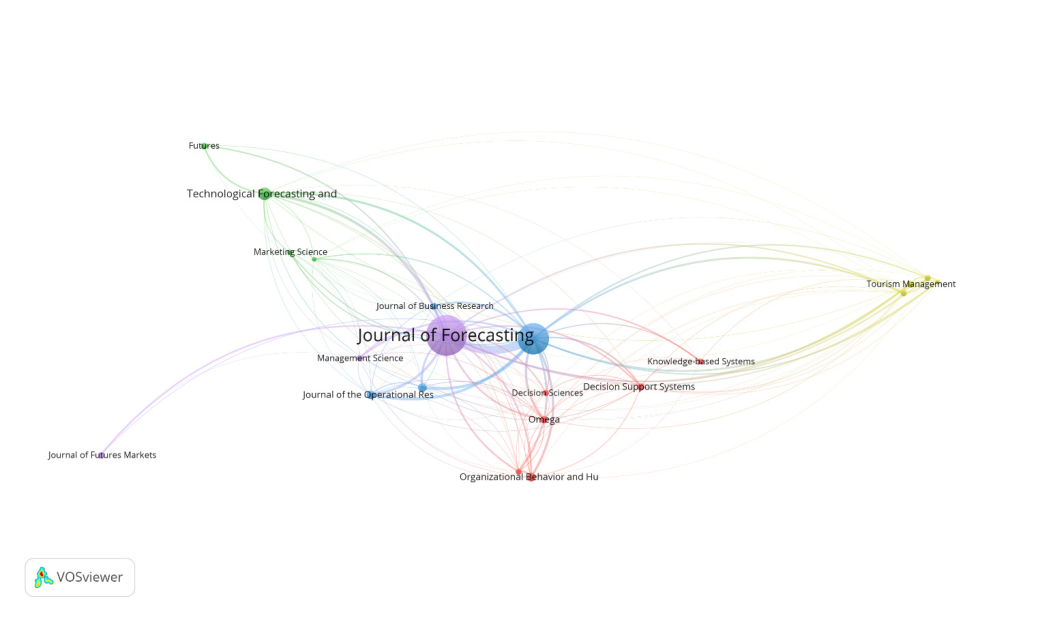
\includegraphics[width=\textwidth]{fig.10.eps}
\caption{JF Journal citation network in Business, Management and Accounting from 1982 to 1994}
\end{figure}

\newpage

\noindent 3.2.2.2. Journal citation network in Economics, Econometrics
and Finance

21 Journals that have no less than 40 publications and 500 citations are
selected to map the JF journal citation network in Economics,
Econometrics and Finance. The citation networks based on the JF papers
and their citing papers belonging to Economics, Econometrics and Finance
are depicted in Fig. 11, and the detailed information about the journal
network is stated in the table 15. JF locates in the center of the
journal network with other journals around it. International Journal of
Production Economics is the citing journal that locates far away from
the other journals, which denotes the content similarity between
International Journal of Production Economics and other connected
journals is much smaller. From the table 15, Applied Economics has the
highest percentage of citing papers, while the remaining journal all
have percentage lower than 50\%.

\begin{figure}[htbp]
\centering
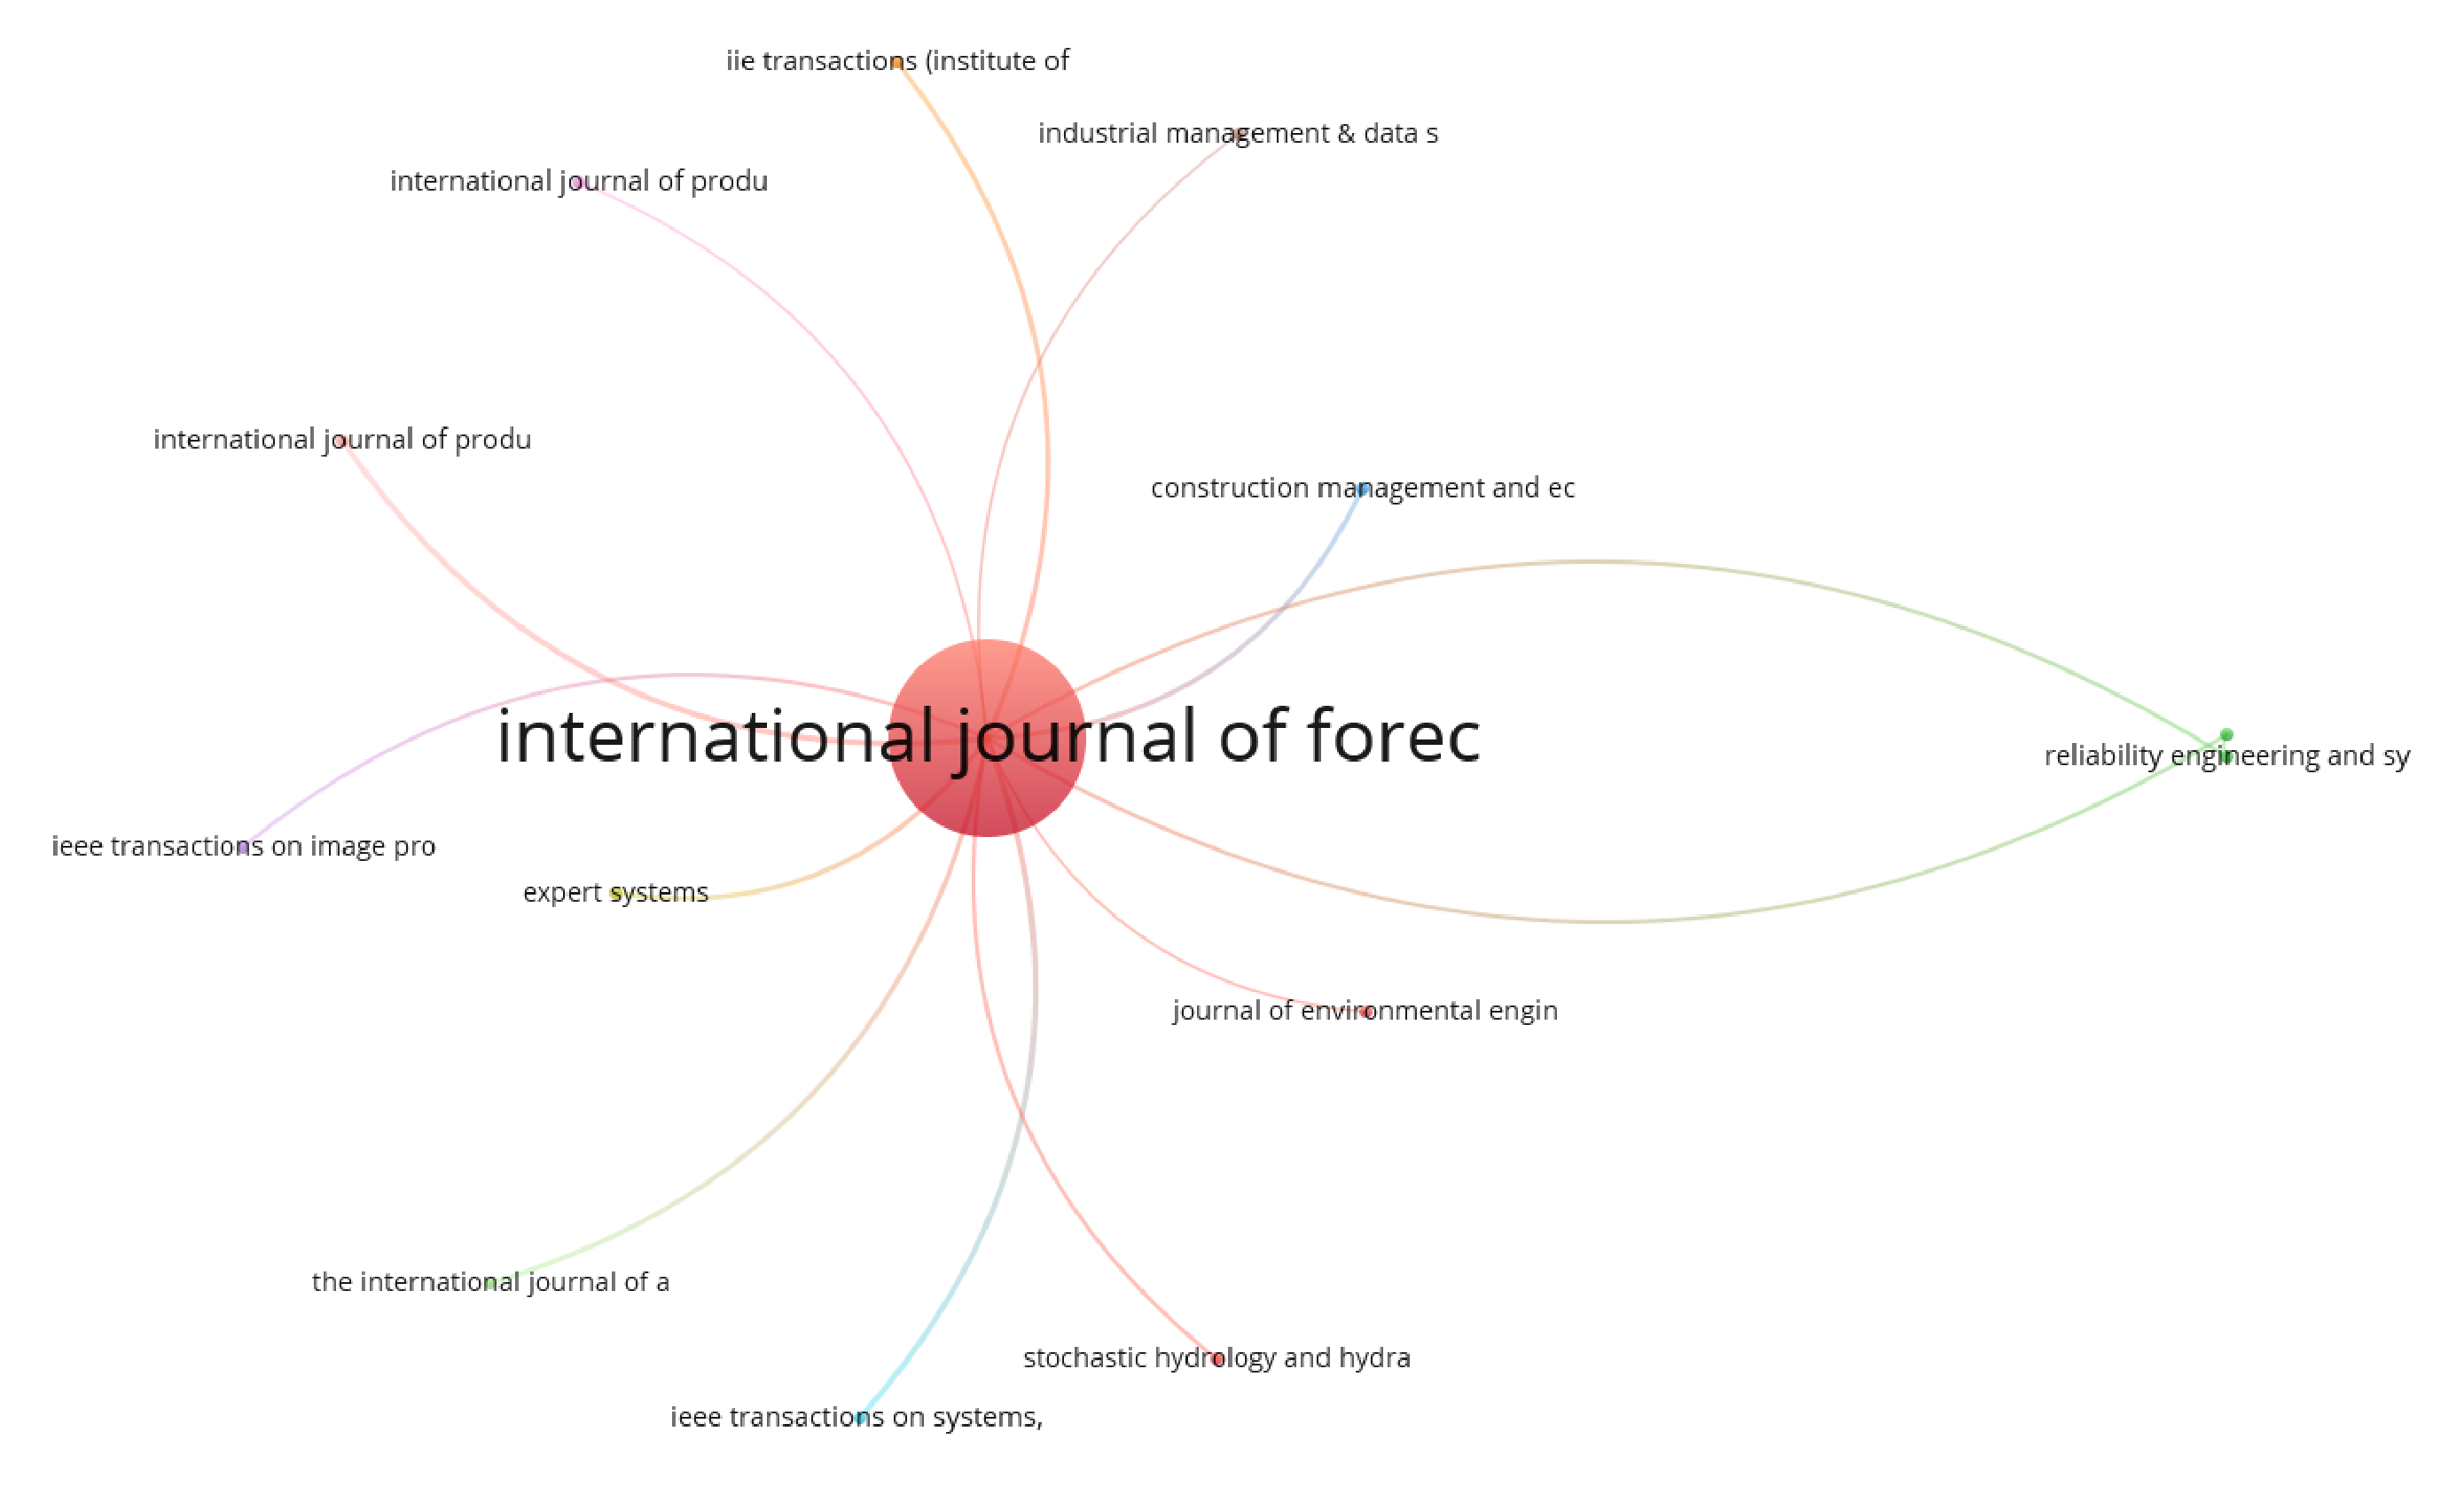
\includegraphics[width=\textwidth]{fig.11.eps}
\caption{JF Journal citation network in Economics, Econometrics and Finance}
\end{figure}

\tablen  

\newpage

\noindent 3.2.2.3. Journal citation network in Mathematics

20 Journals that have no less than 20 publications and 300 citations are
selected to map the JF journal citation network in Mathematics. As shown
in Fig. 12, the journal citation relationships between JF papers and
their citing papers in Mathematics are mapped based on the journal
citation network. In Fig. 12, JF locates in the center of the journal
citation network, and the remaining journals are all around JF. No
journal exists as a big node or linking with JF thickly, which indicates
no citing journal has a prominent performance in this journal citation
network. This point also can be confirmed from the table 16. All of the
citing journals have less than 1,000 links in this journal citation
network, and the majority of them have an approximately 50\% of citing
papers related to JF. European Journal of Operational Research has the
highest percentage of citing papers with 75.84\%, and Journal of Applied
Statistics ranks second in citing paper percentage with 70.12\%.

\begin{figure}[htbp]
\centering
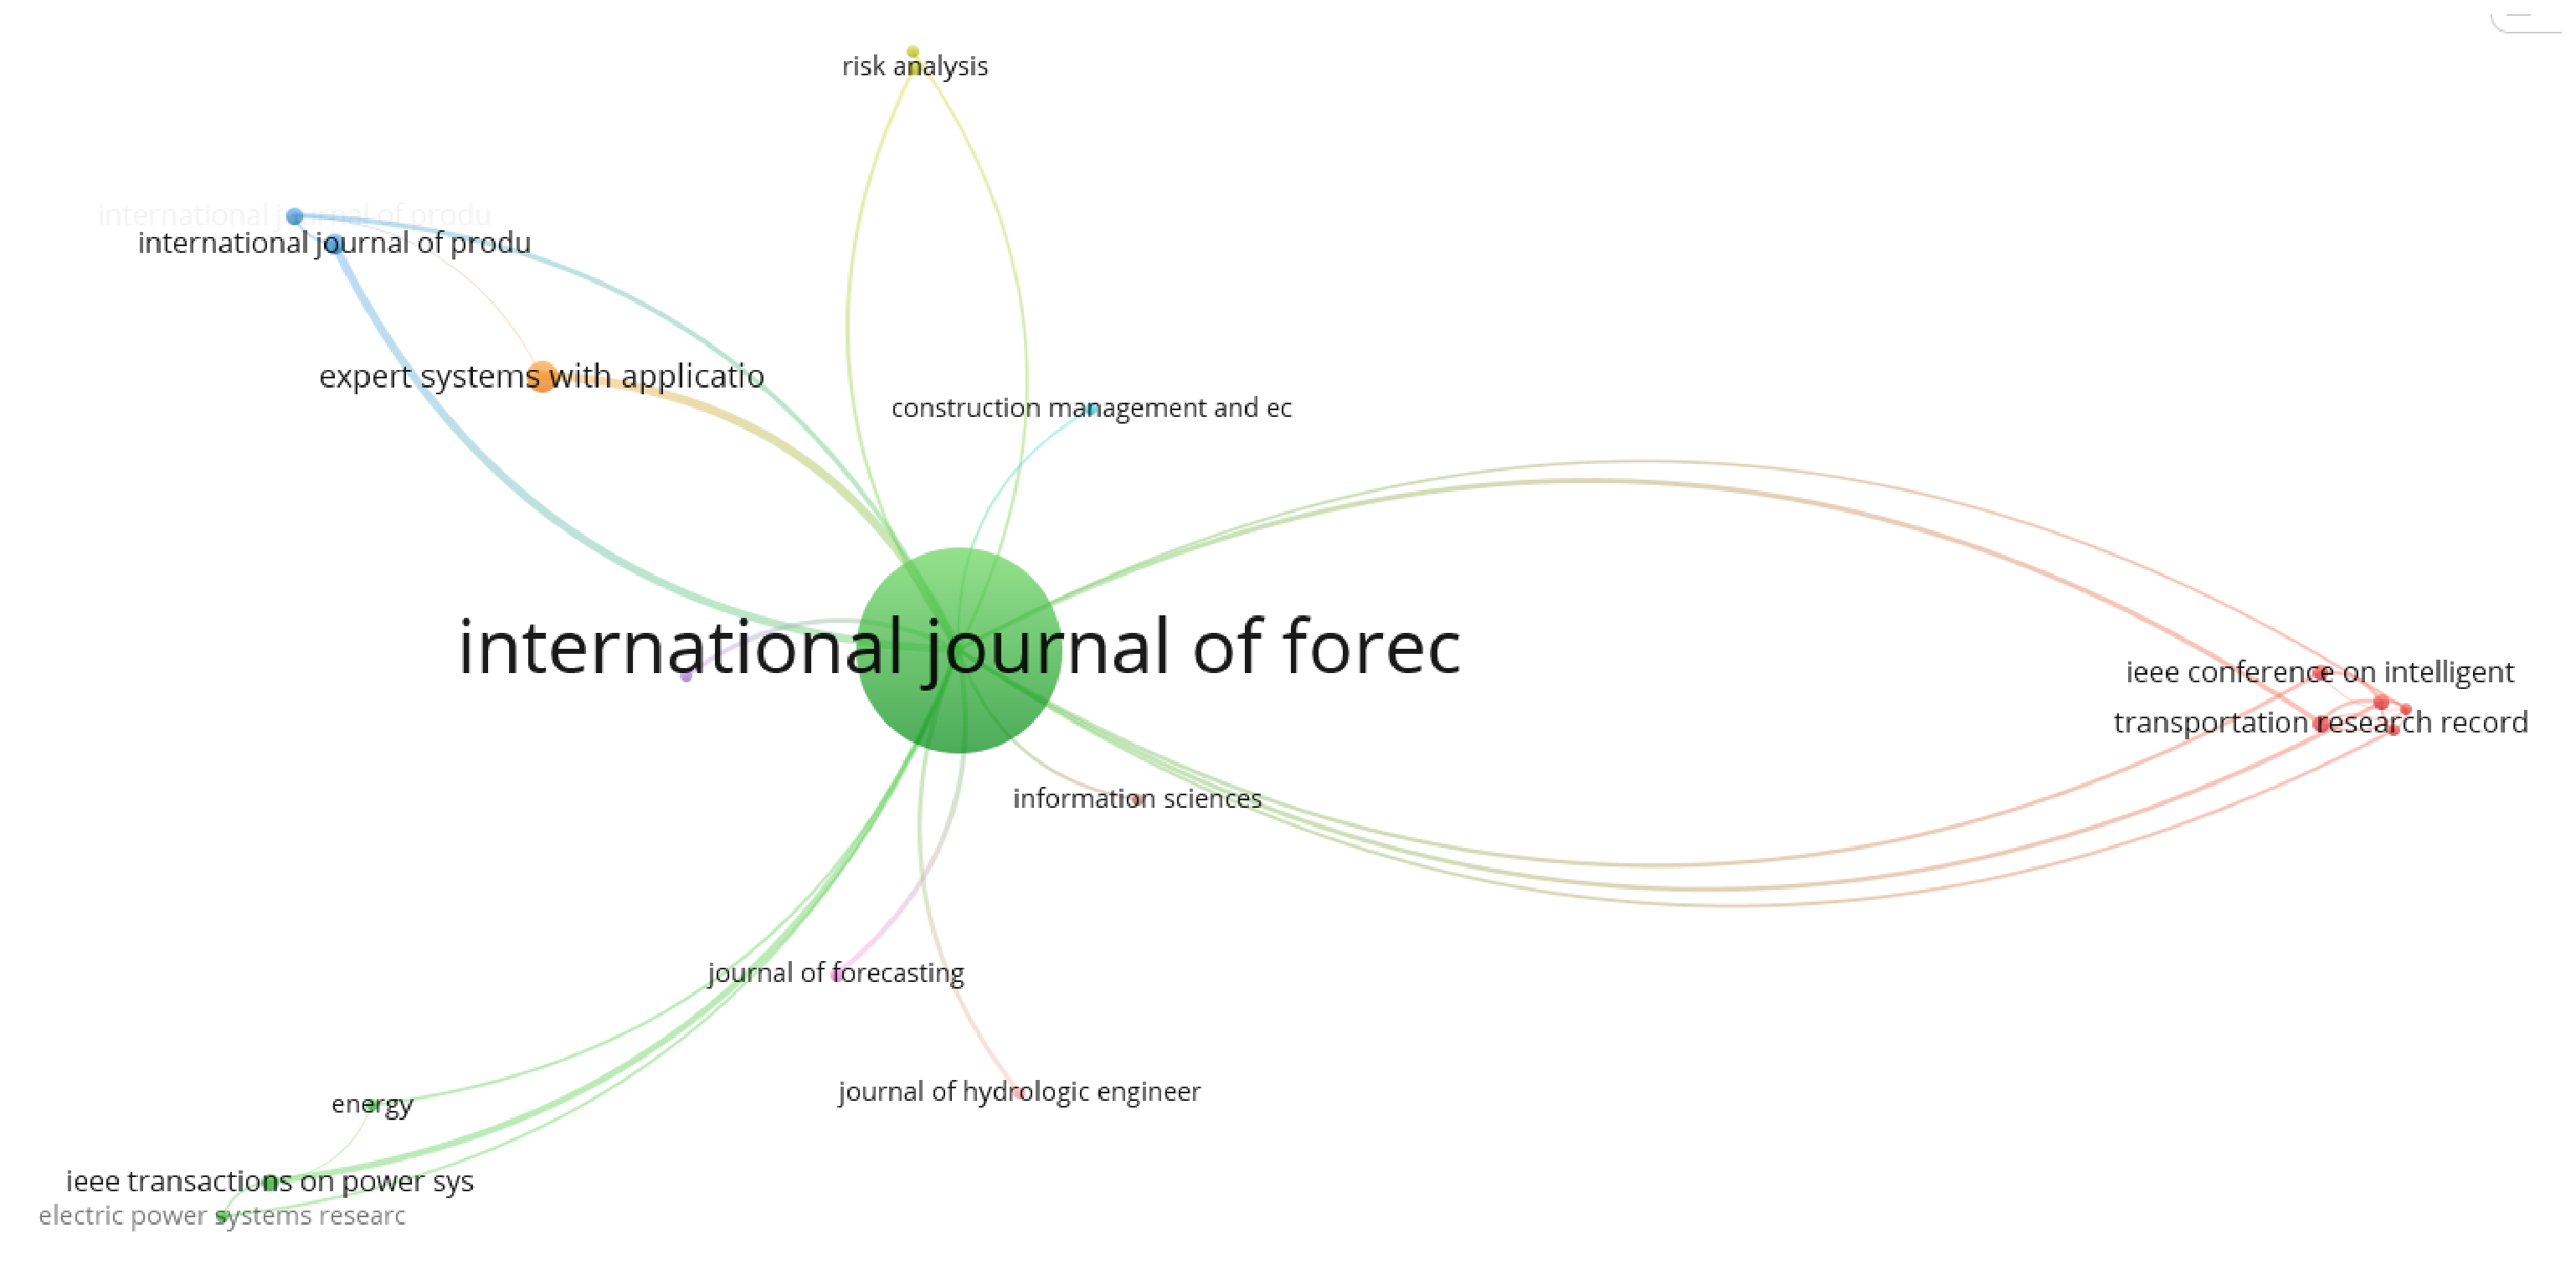
\includegraphics[width=\textwidth]{fig.12.eps}
\caption{JF Journal citation network in Mathematics}
\end{figure}

\tableo

\section{Conclusion and discussion}\label{conclusion-and-discussion}

It has been proven that the proposed method combining the basic
bibliometric indicators and the science mapping techniques is effective
to evaluate the merits of a journal. In this papers, this combination
has been used to analyze the state of development of International
Journal of Forecasting (IJF) from different angles. Three factors
influencing the performance of the journal are identified, and we focus
on analyzing the most cited/co-cited papers, the most prolific/cited
authors, and the most prolific/cited countries. Moreover,
citation/co-citation relationships, co-author relationships, country
collaboration relationships between IJF papers and their citing papers
are elaborated based on science mapping techniques.

In addition, a knowledge diffusion analysis is conducted to supplement
the above proposed method. Based on this knowledge diffusion analysis,
the researches outside the forecasting field can be identified through
investigating the intellectual radiation impact of the forecasting
researches. The analysis supports a valuable direction for the future
forecasting researches. As the leading journals in the forecasting
field, IJF and Journal of Forecasting (JF) papers are all included.
Through investigating the citation relationships between IJF papers and
their citing paper, four typical citing subject areas which are Computer
Science, Engineering, Psychology, and Decision Sciences have been
selected. The journal citation relationships between IJF and the
journals belonging to these four citing subject areas are delineated
through journal citation networks. Similar work is conducted between JF
papers and their citing papers, and we derive five typical citing
subject areas which are Computer Science, Economics, Econometrics and
Finance, Engineering, Psychology, and Decision Sciences. Also the
journal citation networks are constructed to explore the relationships
between JF and the journals belonging to the five citing subject areas.
Besides, the citing subject areas which have a special performance both
in IJF and JF are chosen as the overlapping citing subject areas, and
they are Computer Science, Engineering, Psychology, and Decision
Science. We investigate the IJF papers which are cited by the most
journals within these four subject area, and the derived findings can
answer the question how the IJF researches being cited in the papers
outside the forecasting field behave and what kind of forecasting
knowledge diffuses more widely to the researches outside the forecasting
field.

\noindent Appendix

\noindent Section A: IJF journal citation networks

\noindent A1: IJF journal citation network in Engineering

21 Journals that have no less than 30 publications and 300 citations are
selected to map the IJF journal citation network in Engineering. Four
parameters are clusters (6), local links (133), link strength (4376),
and items (21).

\begin{figure}[htbp]
\centering
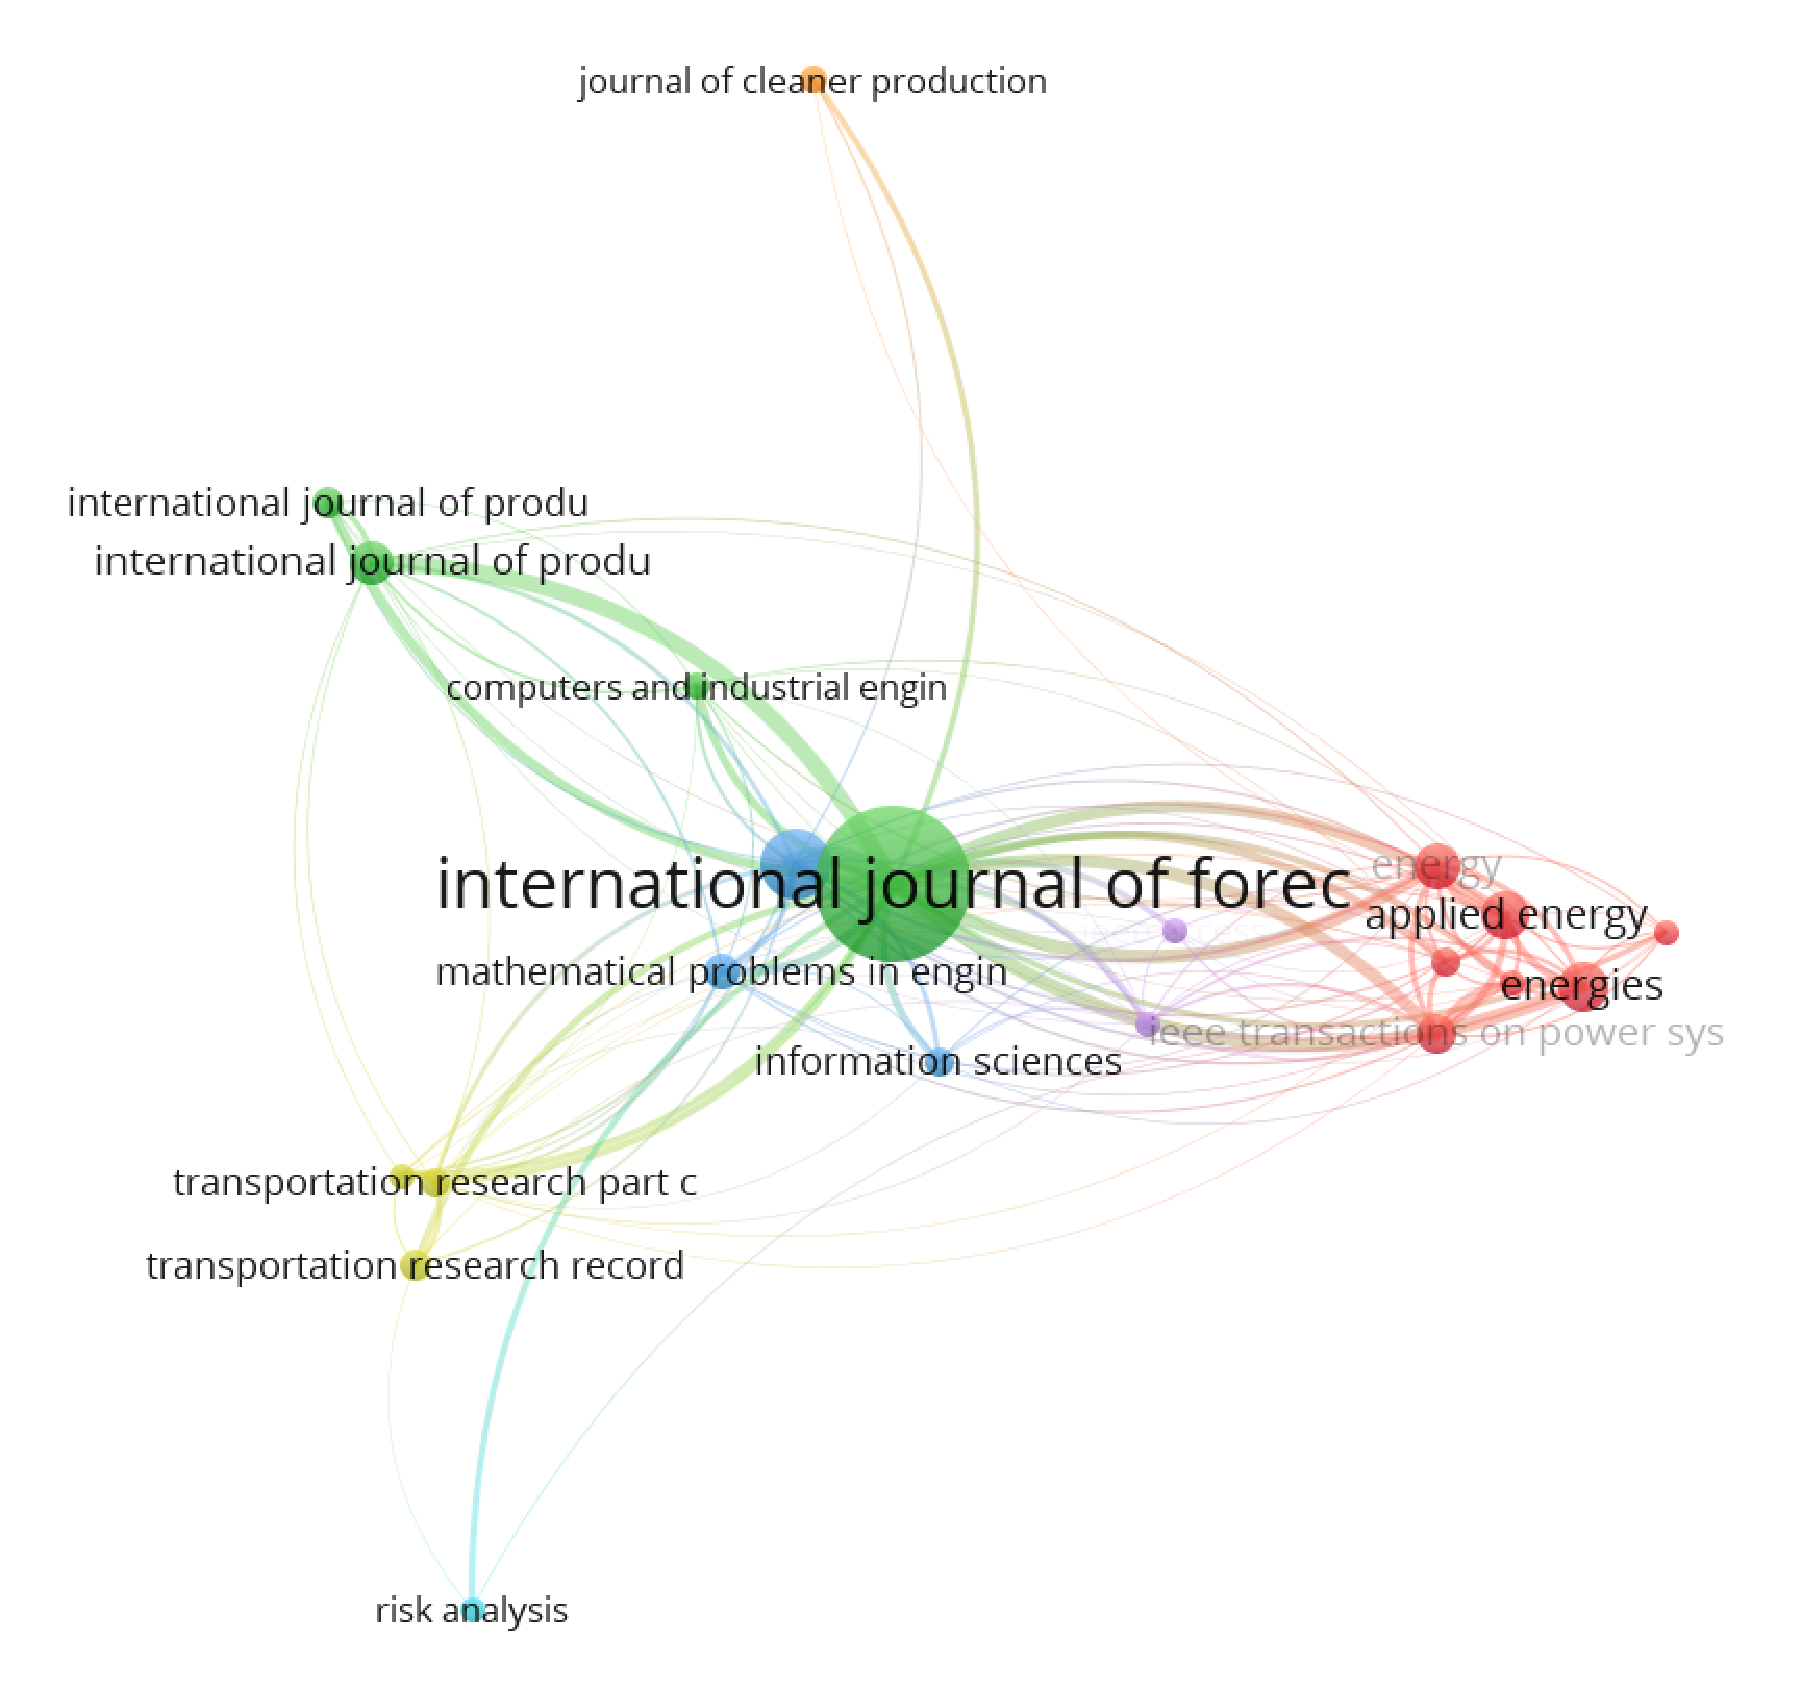
\includegraphics[width=\textwidth]{fig.13.eps}
\caption{IJF journal citation network in Engineering}
\end{figure}

\tablep

\noindent A2: IJF journal citation network in Mathematics

21 Journals that have no less than 30 publications and 300 citations are
selected to map the IJF journal citation network in Mathematics. Four
parameters are clusters (6), local links (156), link strength (7607),
and items (21).

\begin{figure}[htbp]
\centering
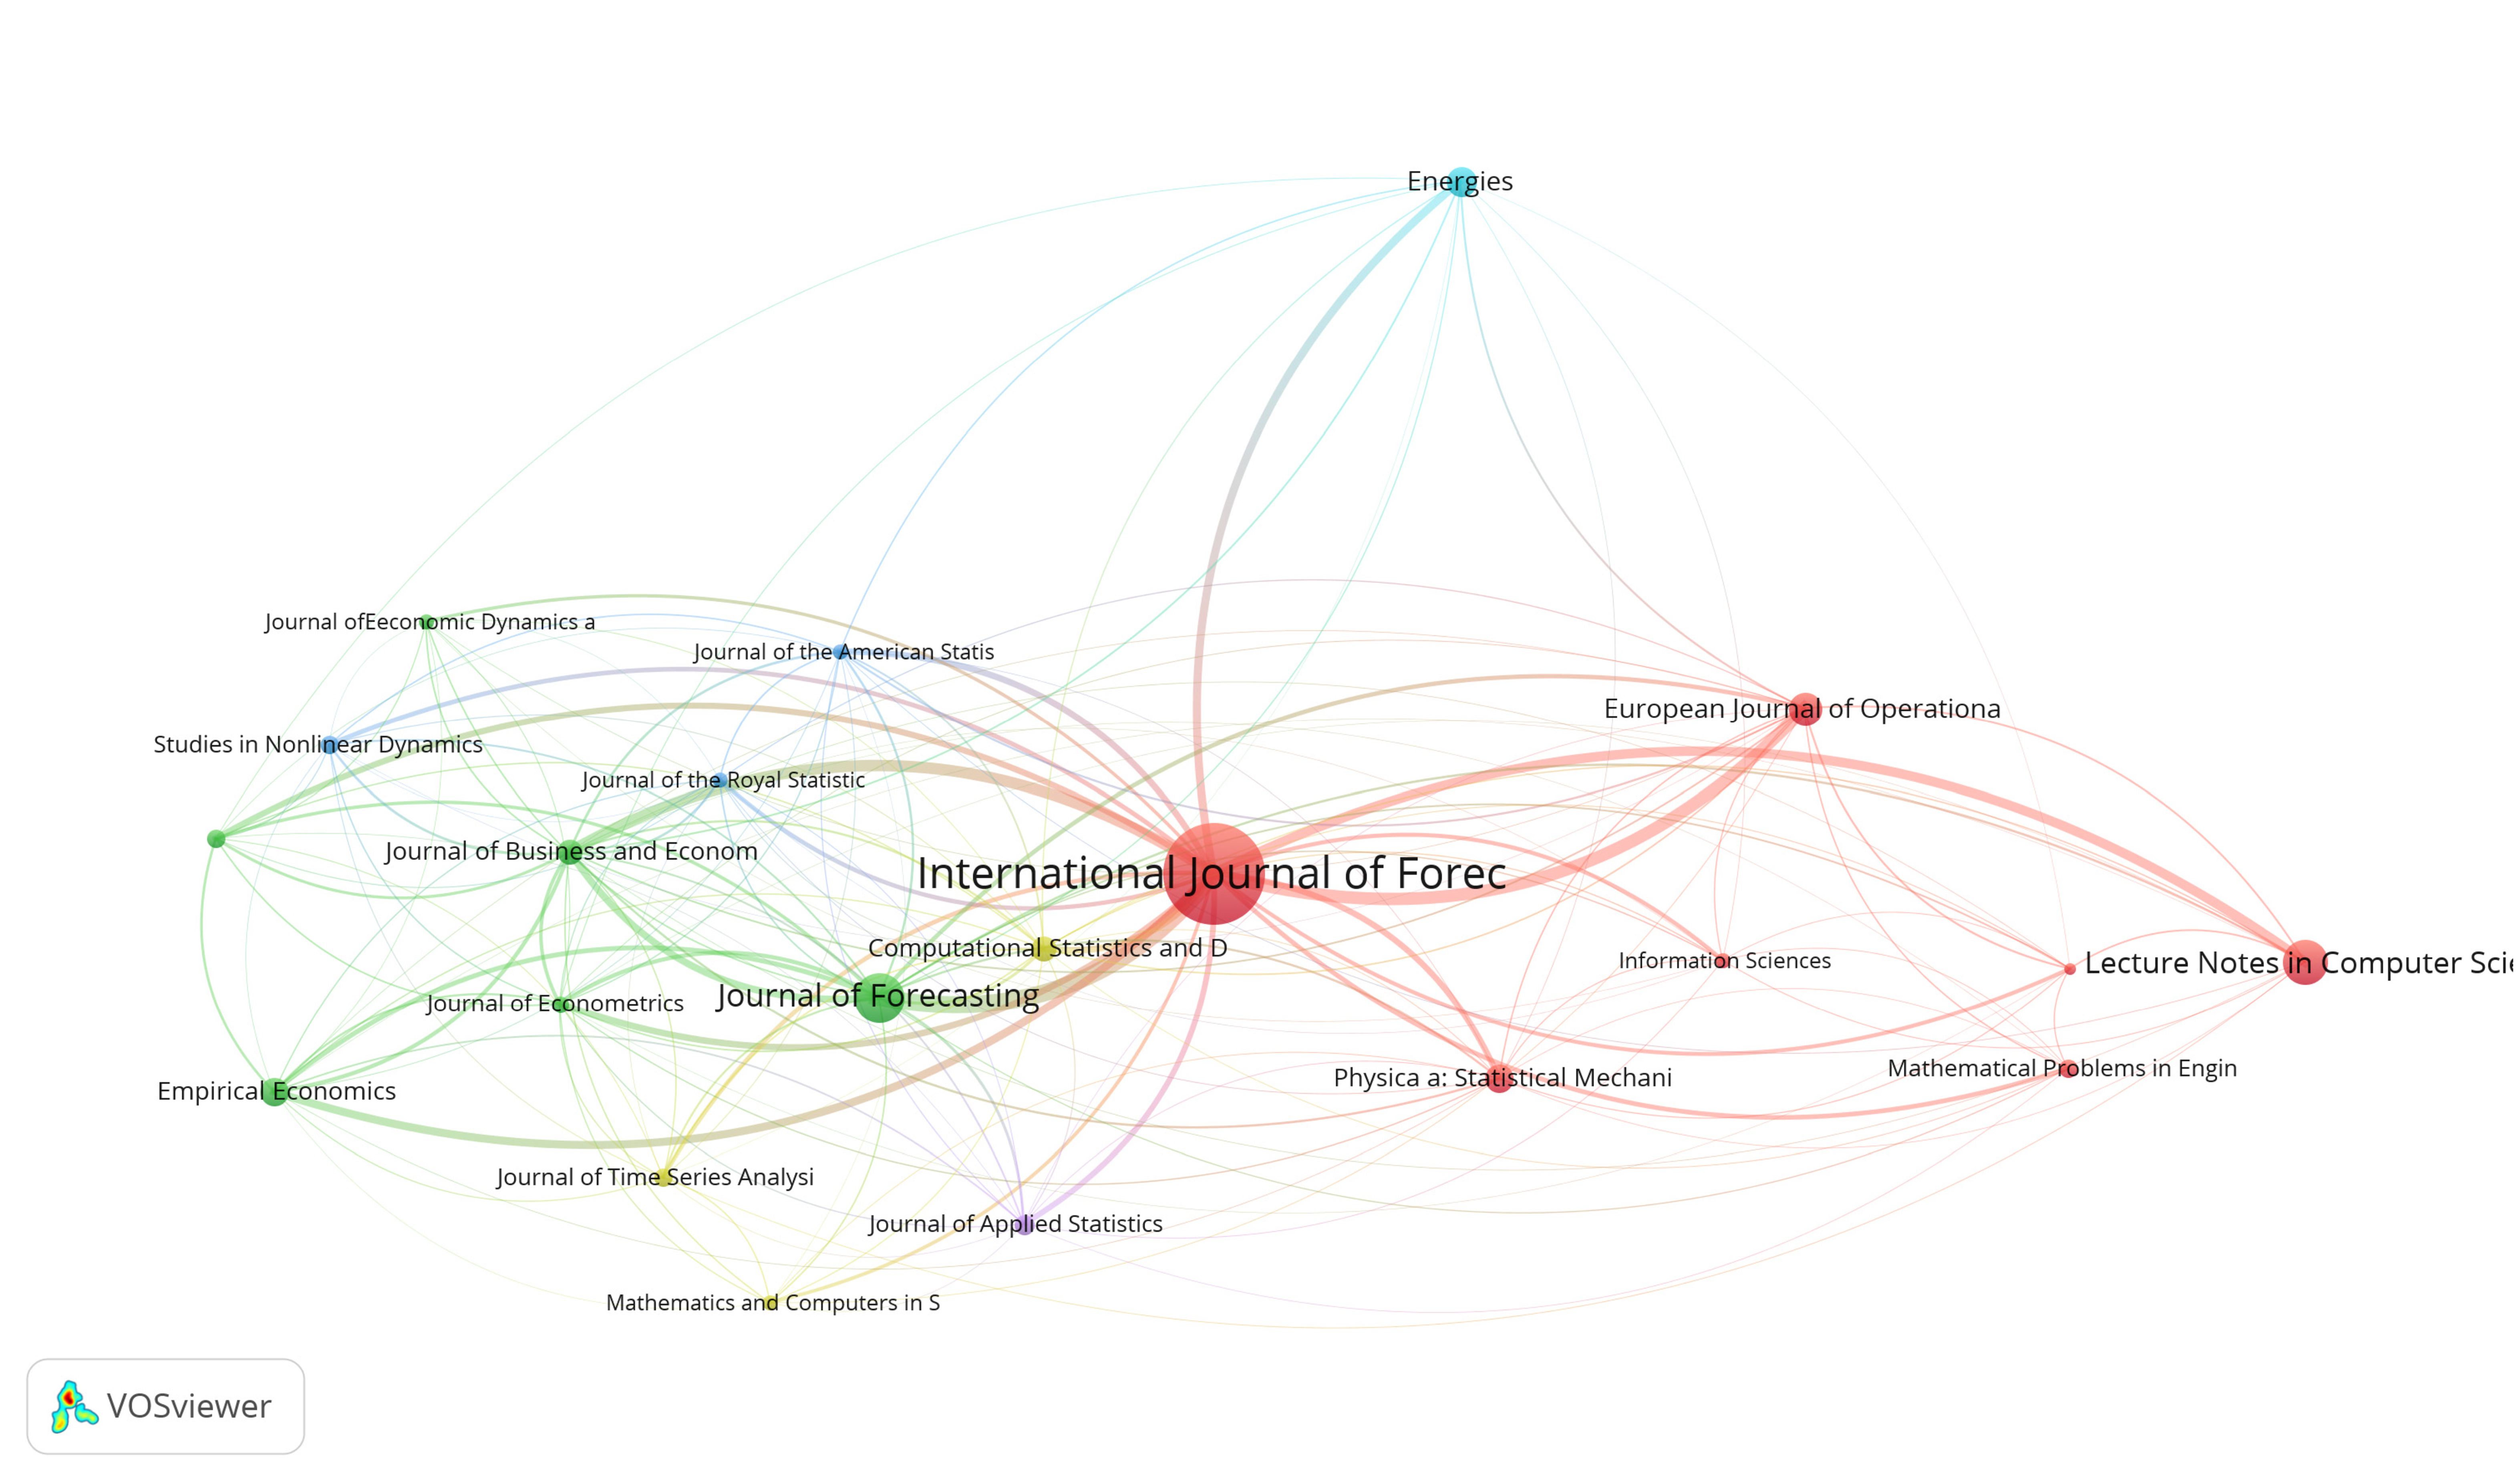
\includegraphics[width=\textwidth]{fig.14.eps}
\caption{IJF journal citation network in Mathematics}
\end{figure}

\tableq

\noindent A3: IJF journal citation network in Social Sciences

21 Journals that have no less than 20 publications and 300 citations are
selected to map the IJF journal citation network in Social Sciences.
Four parameters are clusters (8), local links (87), link strength
(4971), and items (21).

\newpage

\begin{figure}[htbp]
\centering
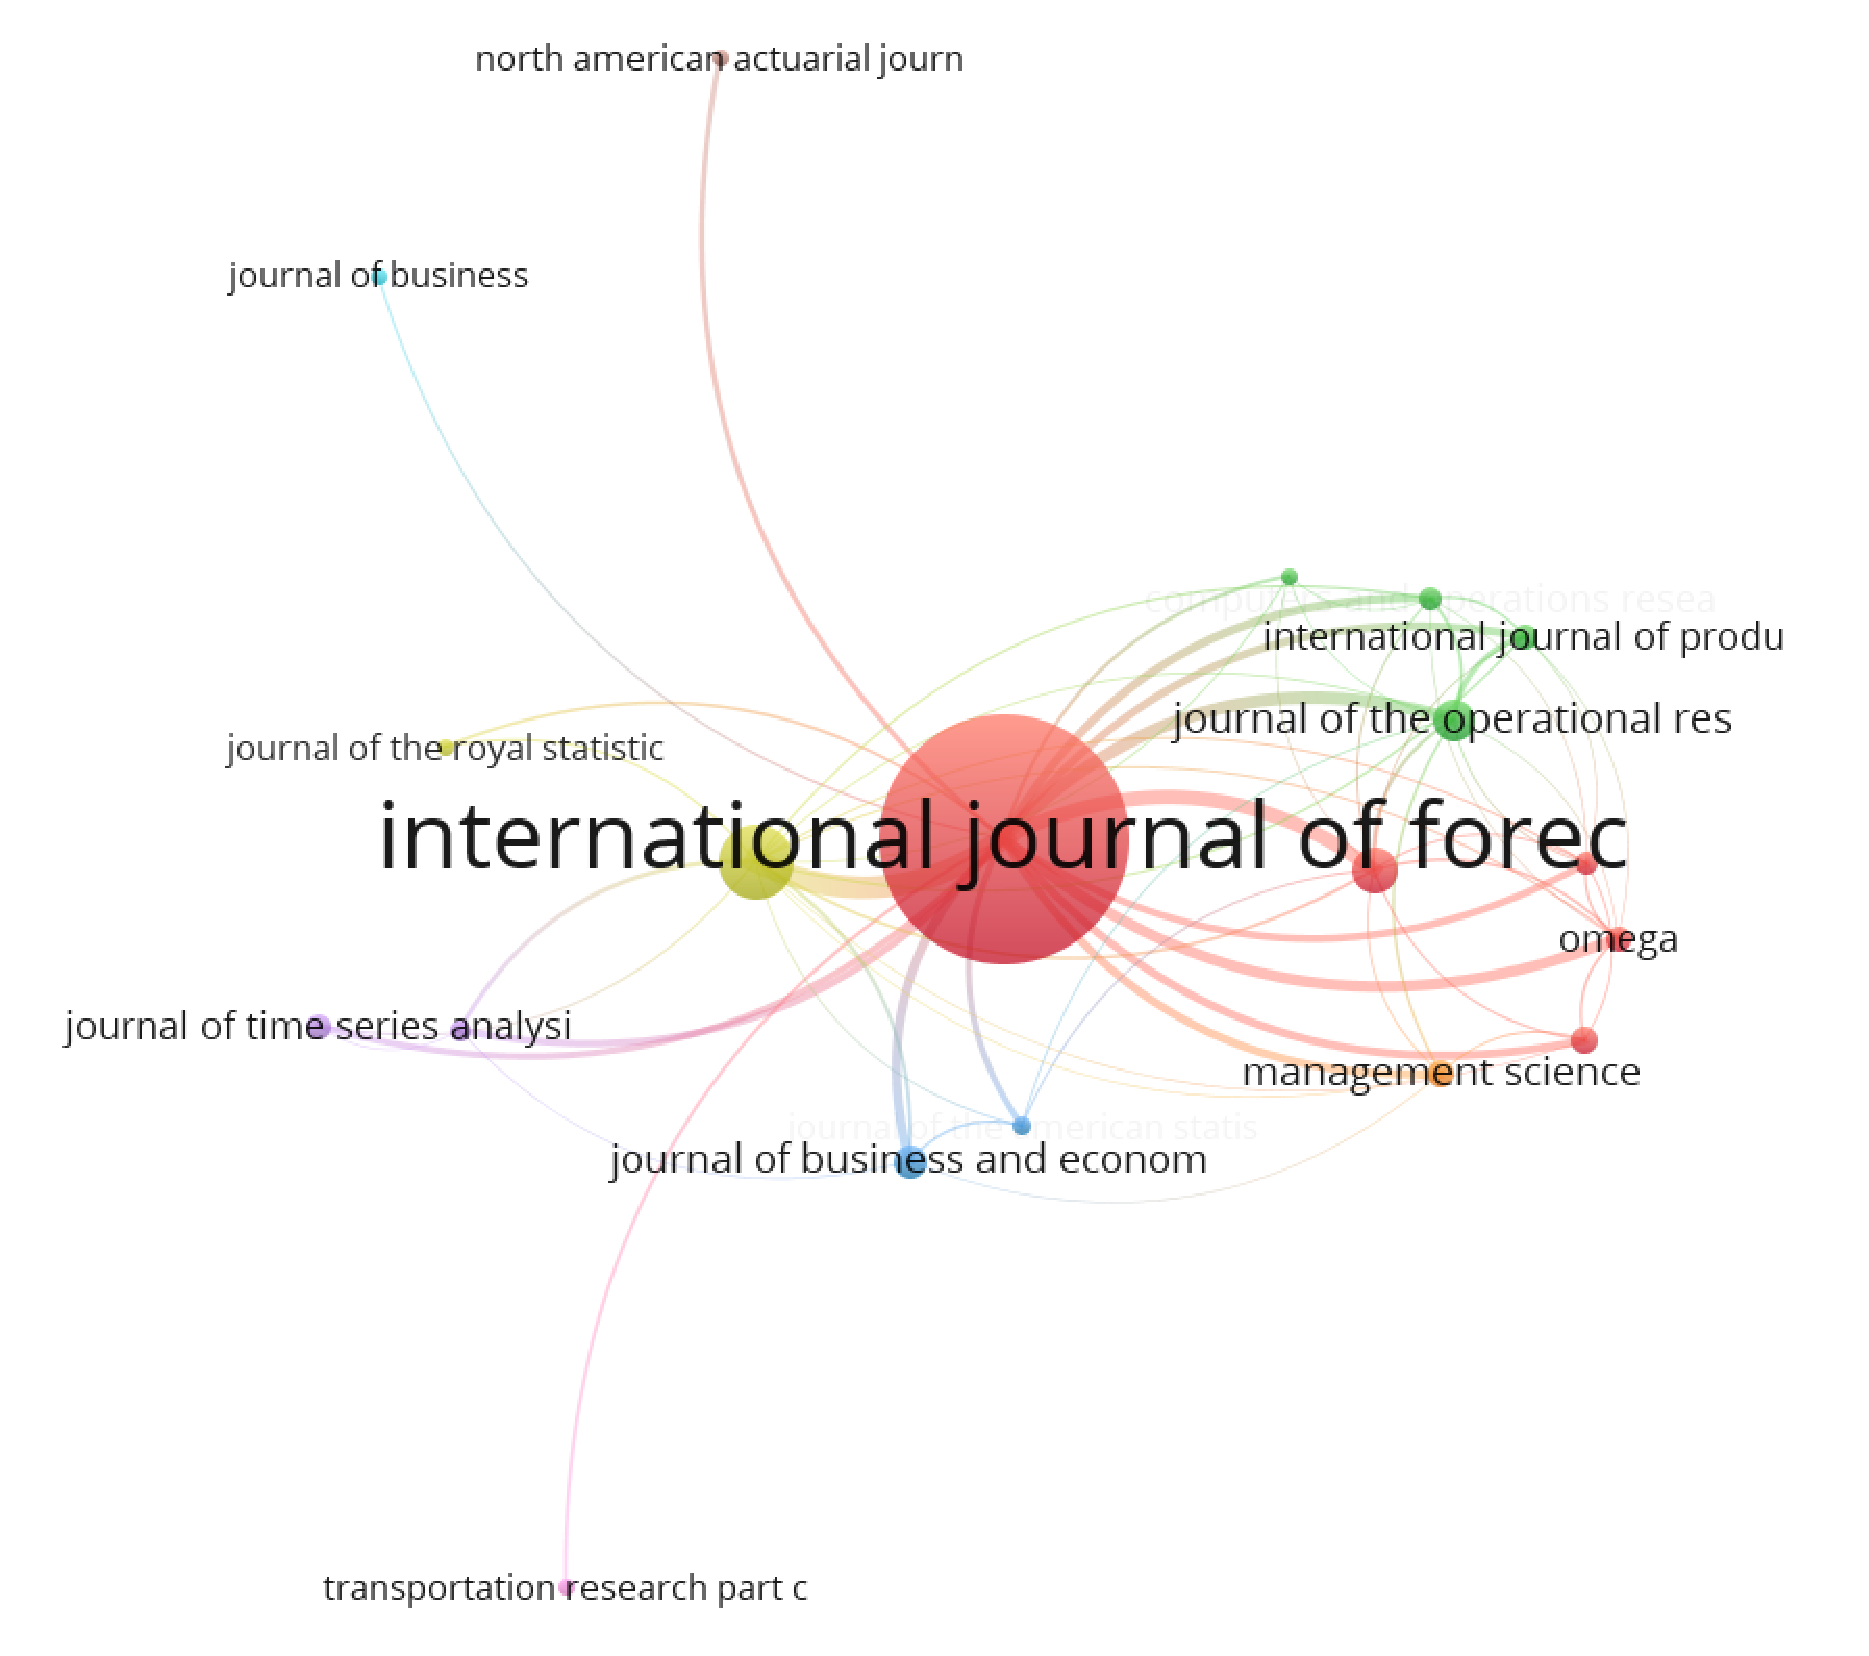
\includegraphics[width=\textwidth]{fig.15.eps}
\caption{IJF journal citation network in Social Sciences}
\end{figure}

\tabler

\noindent A4: IJF journal citation network in Decision Sciences

20 Journals that have no less than 30 publications and 300 citations are
selected to map the IJF journal citation network in Decision Sciences.
Four parameters are clusters (4), local links (138), link strength
(7535), and items (20).

\newpage

\begin{figure}[htbp]
\centering
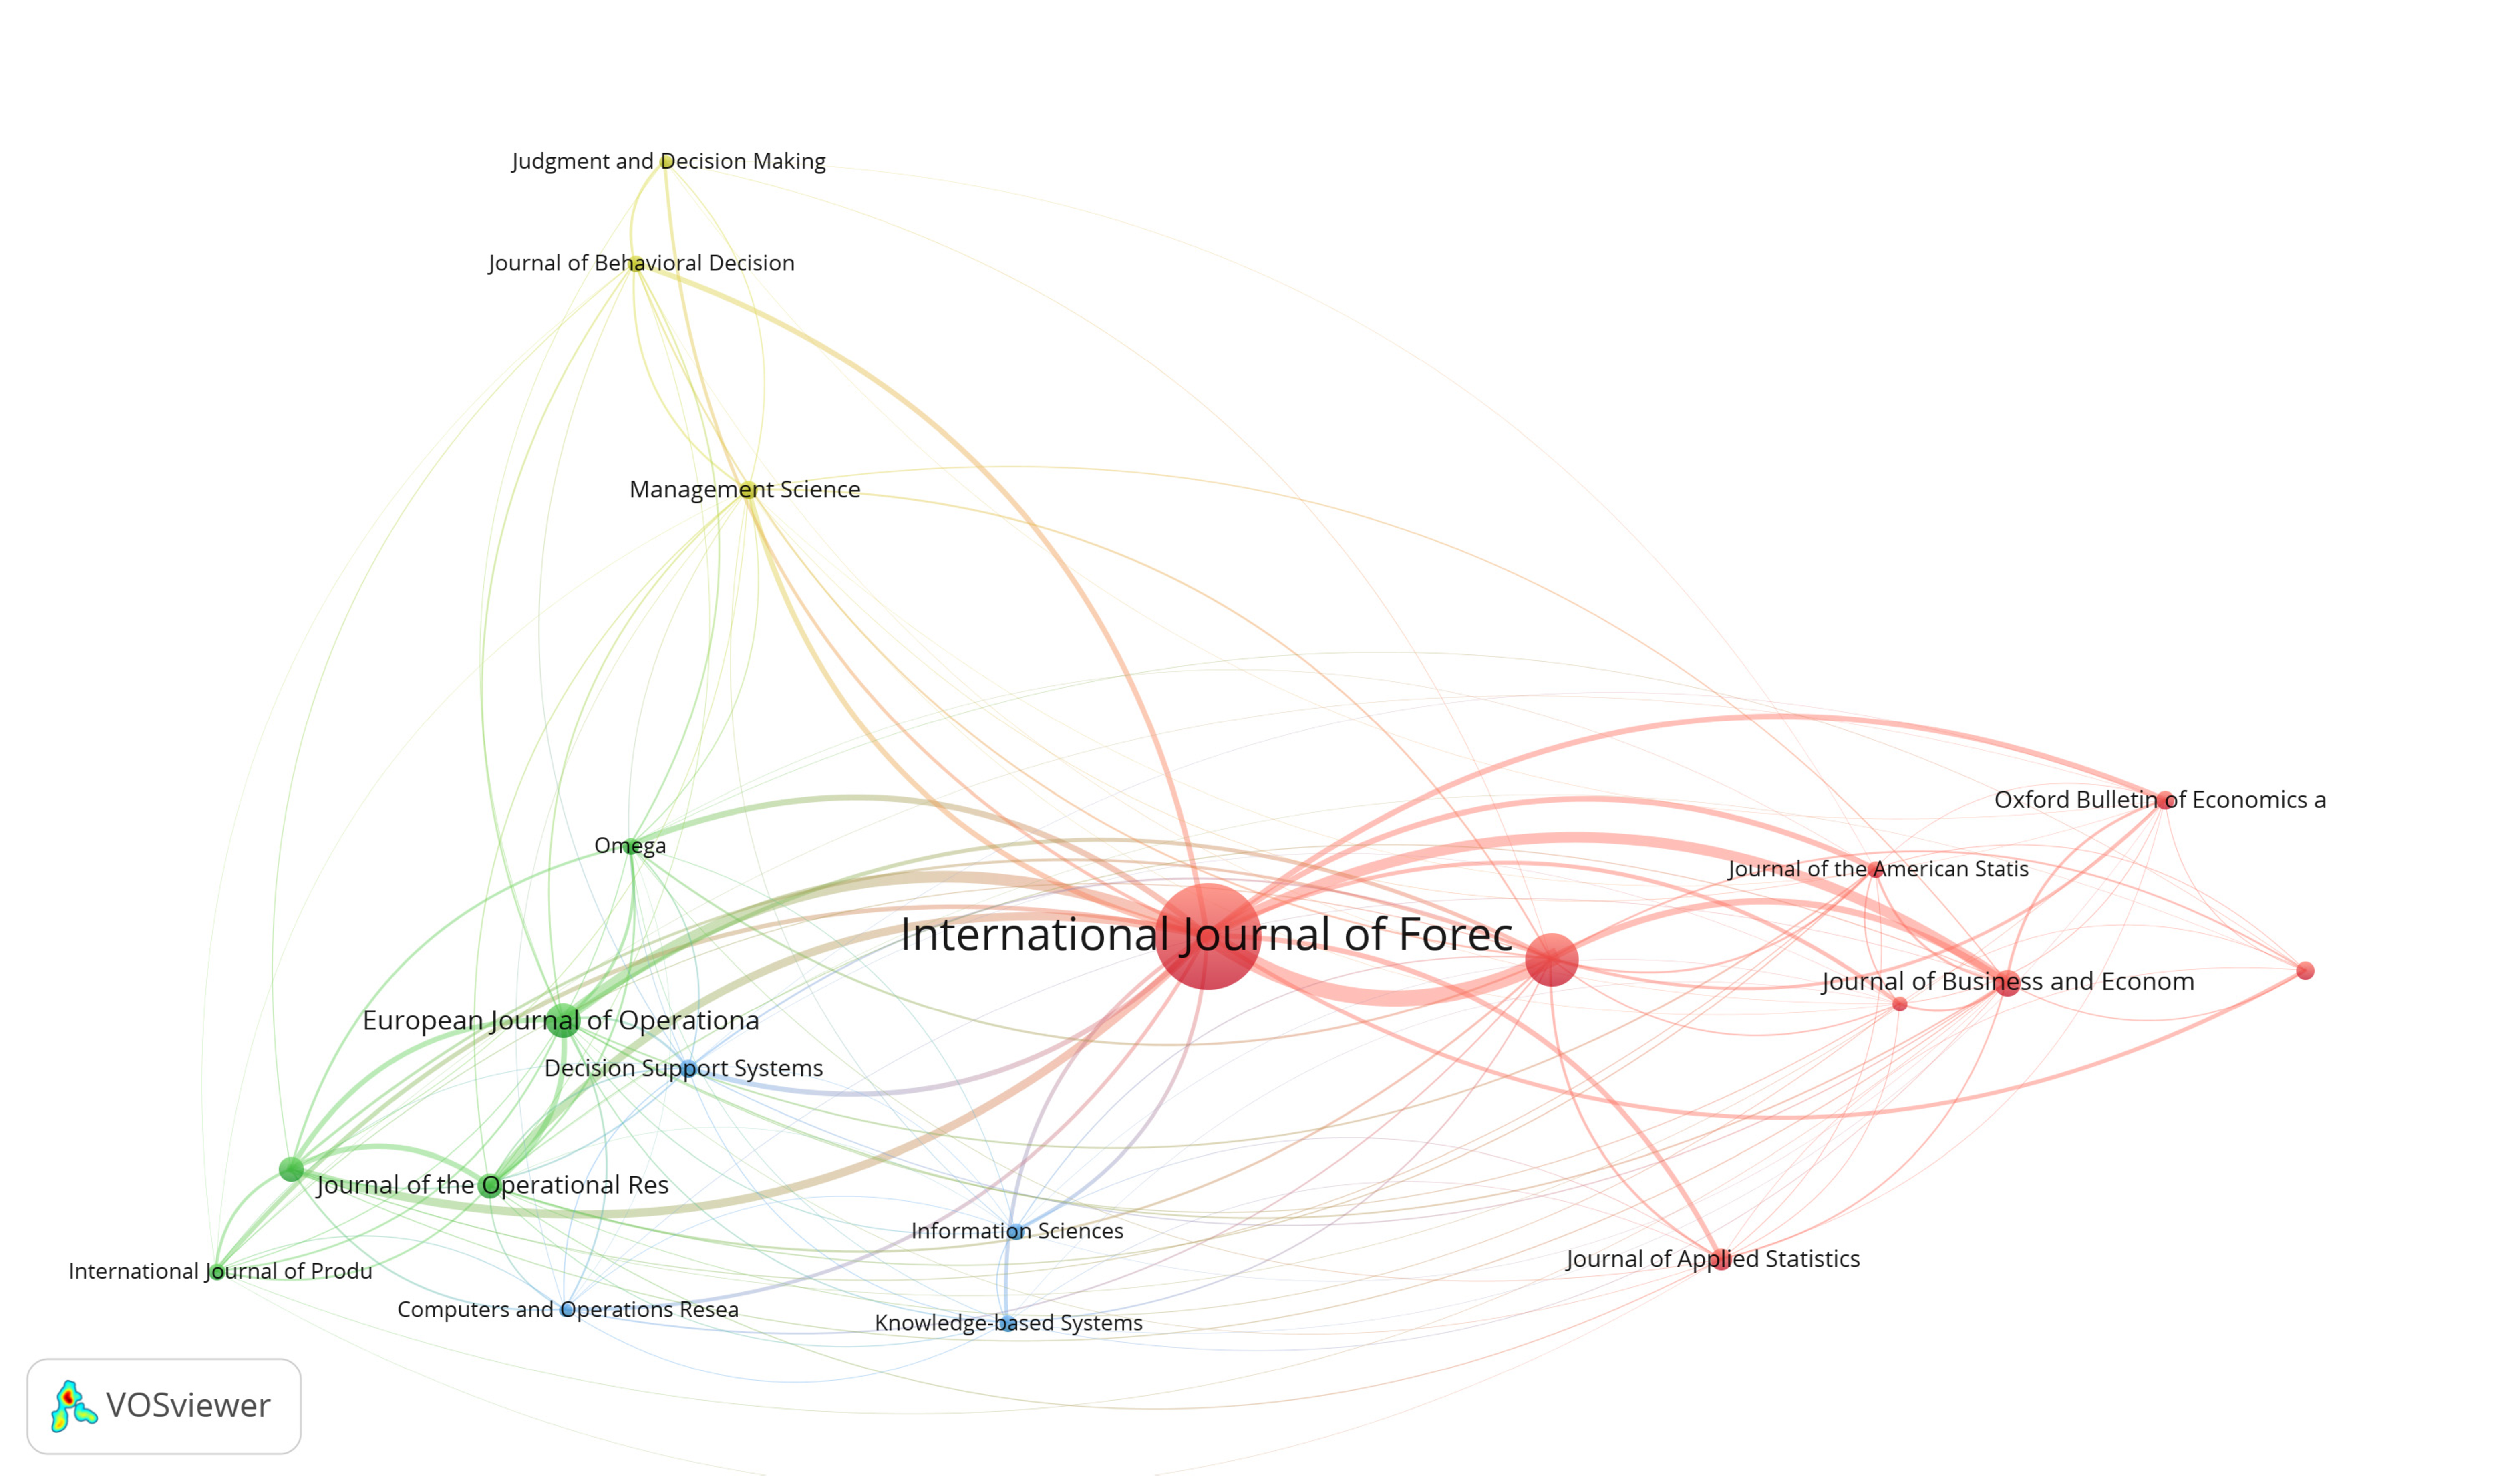
\includegraphics[width=\textwidth]{fig.16.eps}
\caption{IJF journal citation network in Decision  Sciences}
\end{figure}

\tables

\noindent A5: IJF journal citation network in Energy

20 Journals that have no less than 15 publications and 200 citations are
selected to map the IJF journal citation network in Energy. Four
parameters are clusters (4), local links (153), link strength (4734),
and items (20).

\newpage

\begin{figure}[htbp]
\centering
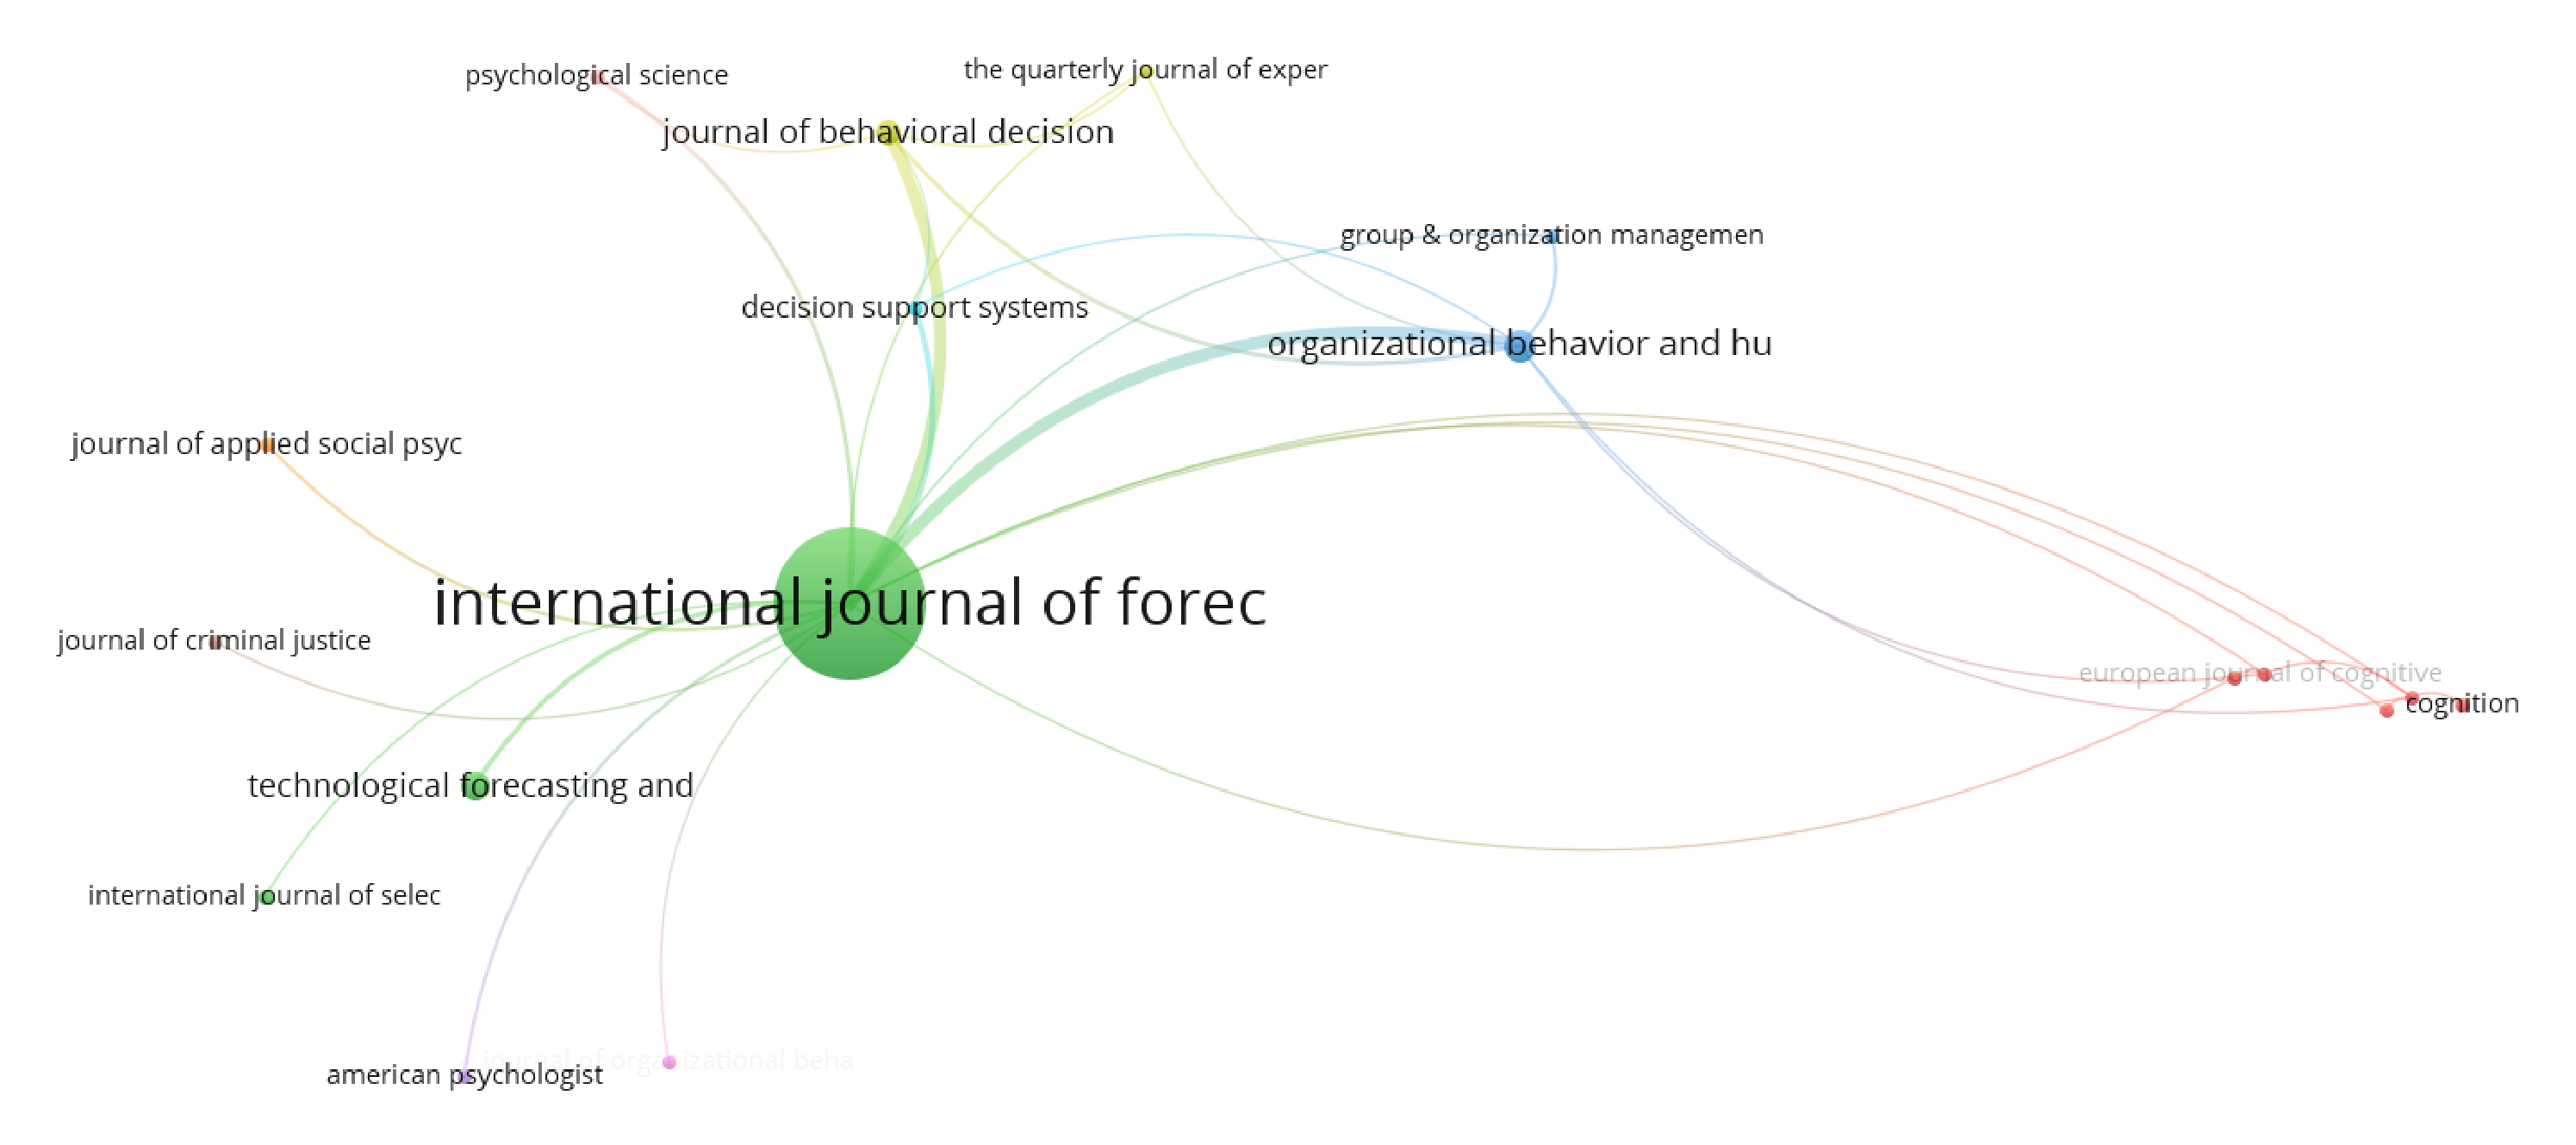
\includegraphics[width=\textwidth]{fig.17.eps}
\caption{IJF journal citation network in Energy}
\end{figure}

\tablet

\noindent A6: IJF journal citation network in Environmental Science

20 Journals that have no less than 15 publications and 180 citations are
selected to map the IJF journal citation network in Environmental
Science. Four parameters are clusters (8), local links (79), link
strength (1568), and items (20).

\newpage

\begin{figure}[htbp]
\centering

\includegraphics[width=\textwidth]{fig.18.eps}
\caption{IJF journal citation network in Environmental Science}
\end{figure}

\tableu

\noindent A7: IJF journal citation network in Earth and Planetary
Sciences

20 Journals that have no less than 15 publications and 180 citations are
selected to map the IJF journal citation network in Earth and Planetary
Sciences. Four parameters are clusters (10), local links (70), link
strength (481), and items (20).

\newpage

\begin{figure}[htbp]
\centering
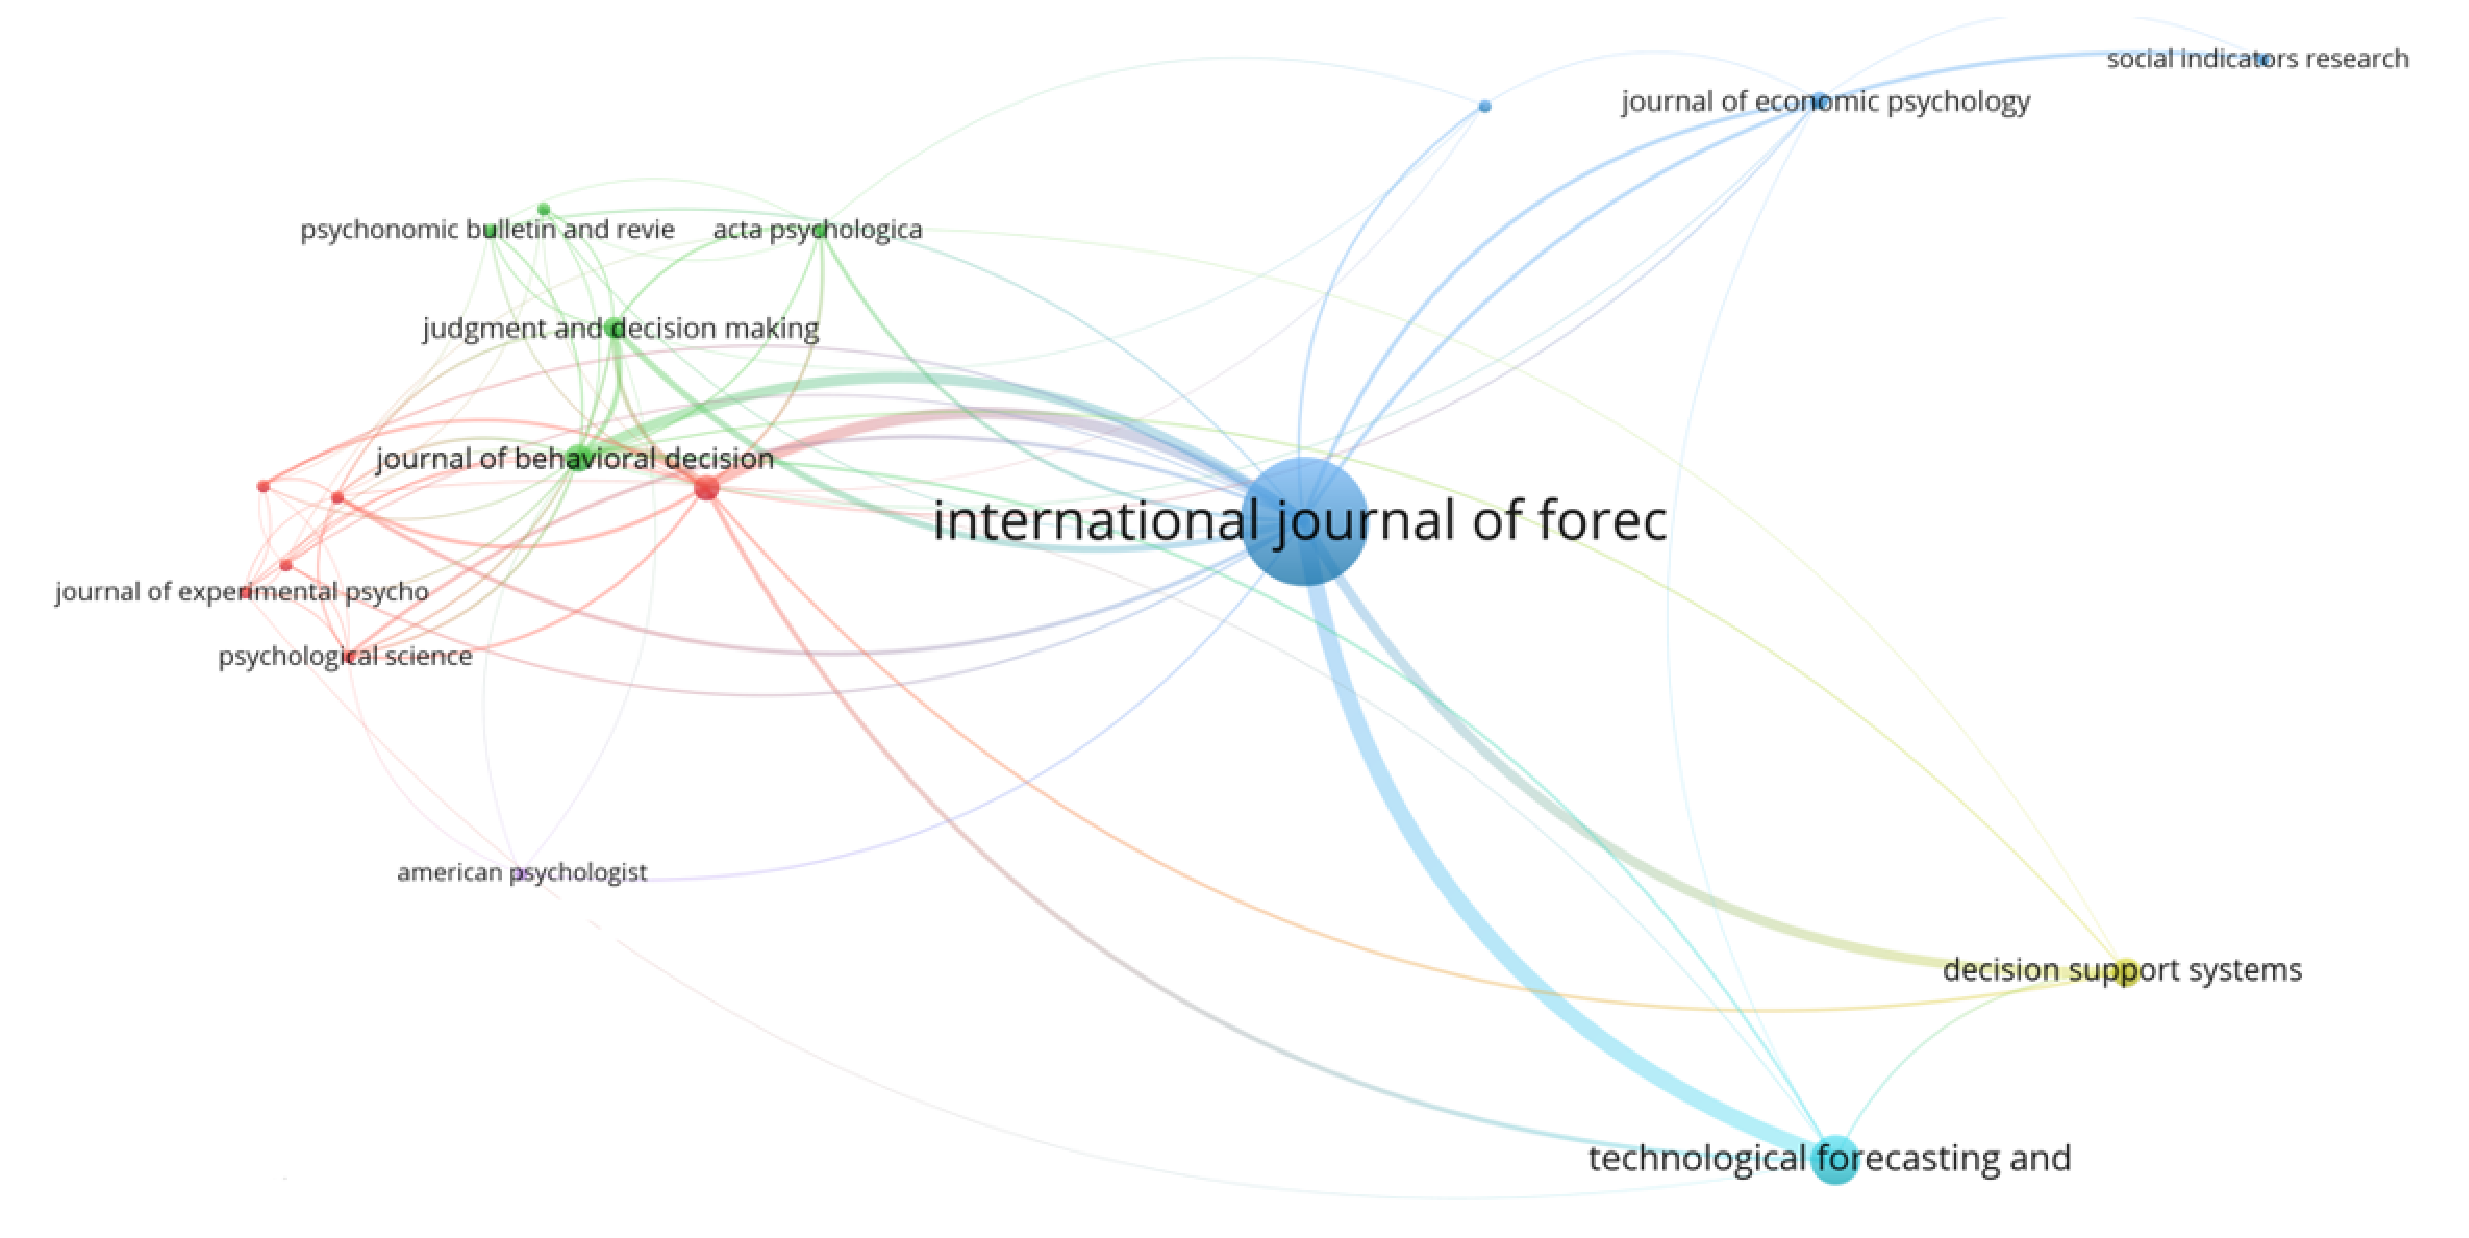
\includegraphics[width=\textwidth]{fig.19.eps}
\caption{IJF journal citation network in Earth and Planetary Sciences}
\end{figure}

\tablev

\noindent Section B: JF journal citation networks

\noindent B1: JF journal citation network in Computer Science

21 Journals that have no less than 15 publications and 100 citations are
selected to map the JF journal citation network in Computer Science.
Four parameters are clusters (10), local links (137), link strength
(1947), and items (21).

\newpage

\begin{figure}[htbp]
\centering
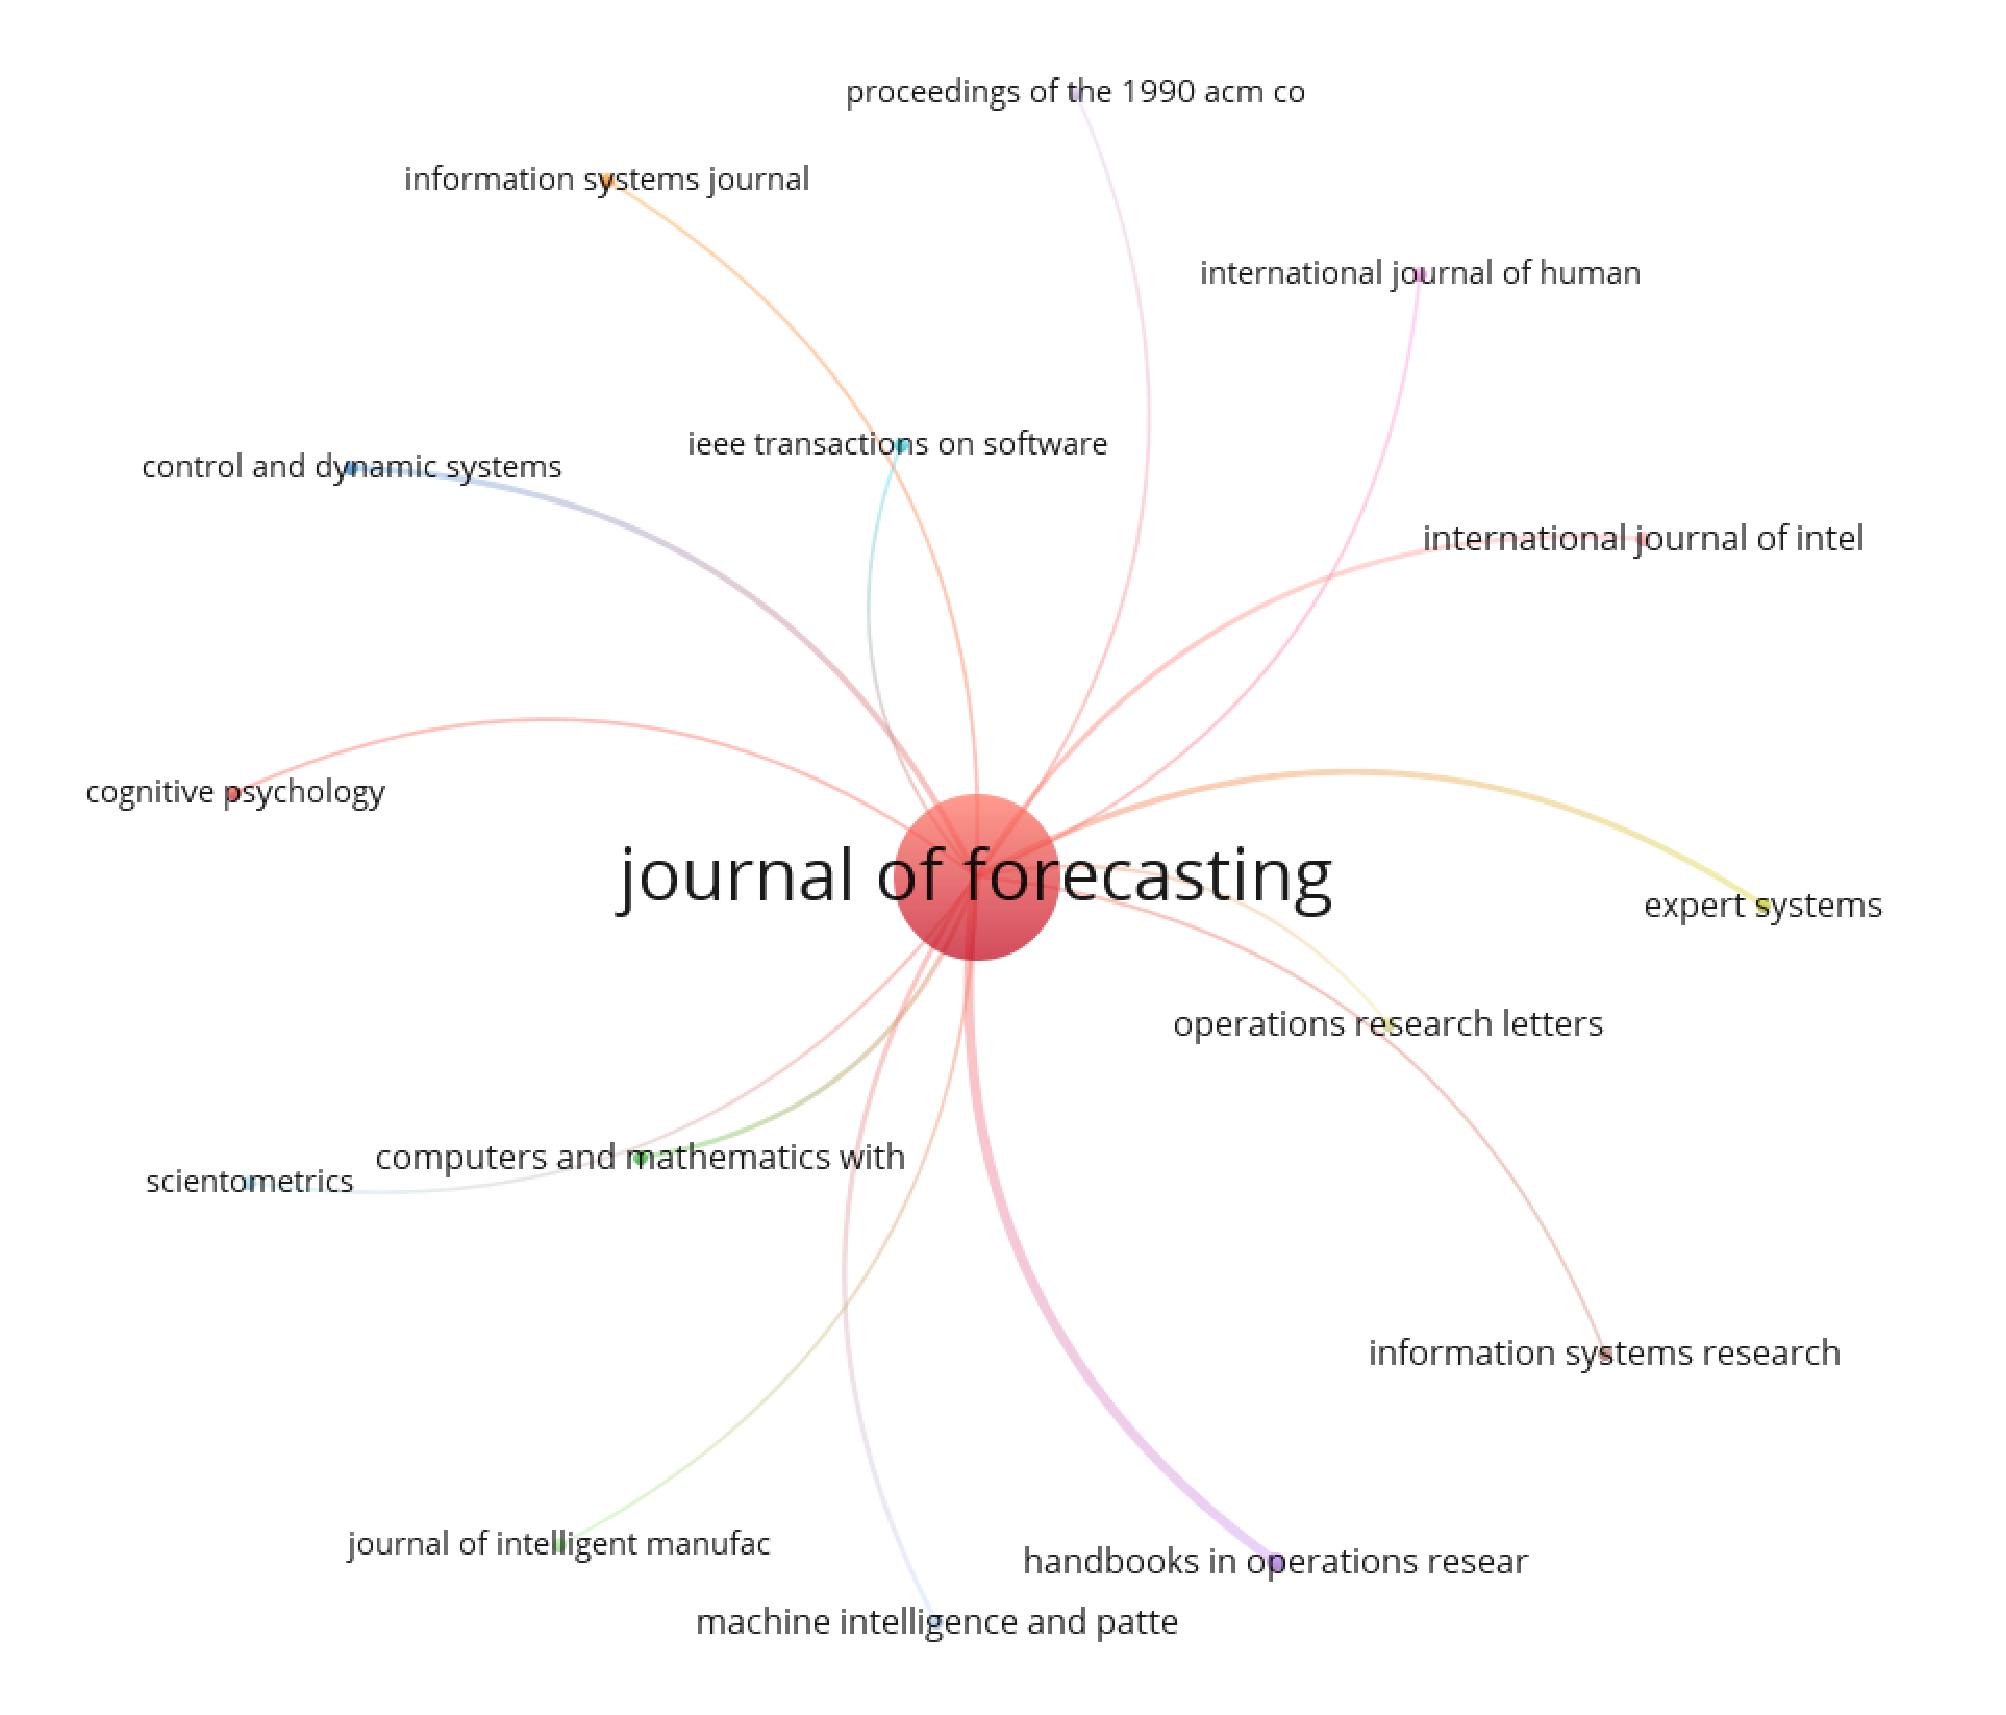
\includegraphics[width=\textwidth]{fig.20.eps}
\caption{JF journal citation network in Computer Science}
\end{figure}

\tablew

\noindent B2: JF journal citation network in Decision Science

20 Journals that have no less than 20 publications and 300 citations are
selected to map the JF journal citation network in Decision Science.
Four parameters are clusters (4), local links (125), link strength
(2978), and items (20).

\newpage

\begin{figure}[htbp]
\centering
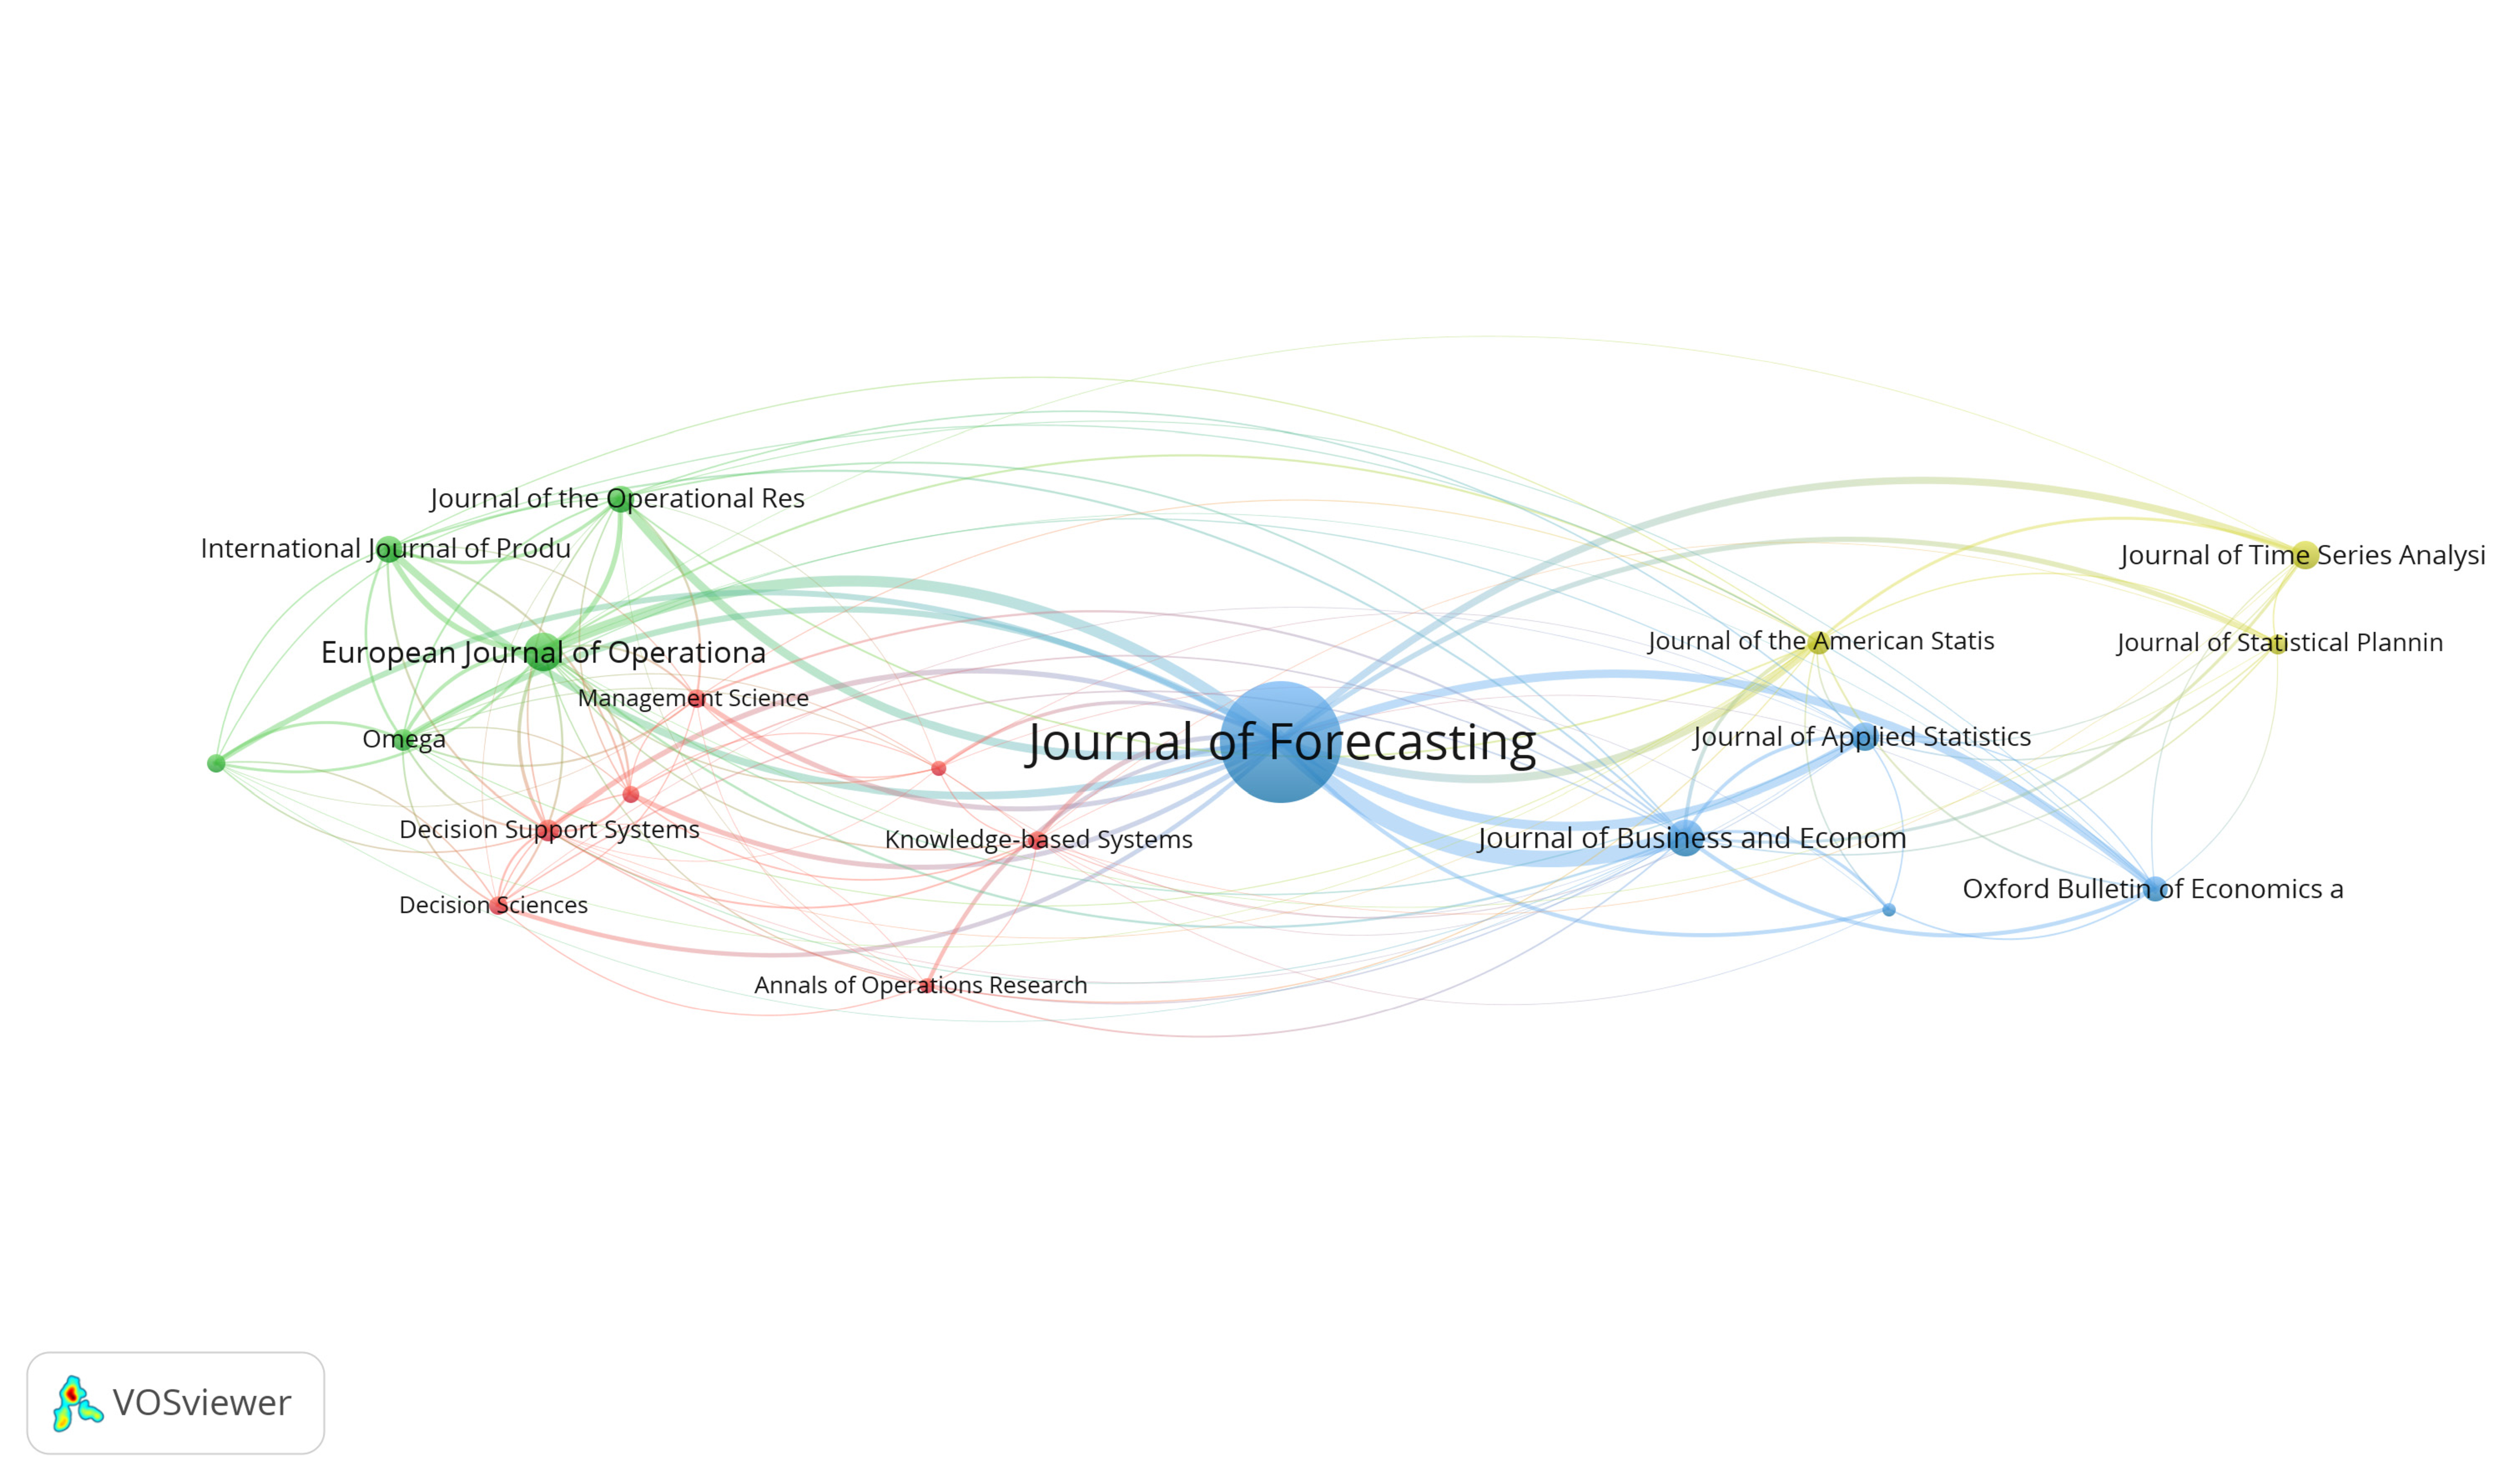
\includegraphics[width=\textwidth]{fig.21.eps}
\caption{JF journal citation network in Decision Science}
\end{figure}

\tablex

\noindent B3: JF journal citation network in Engineering

20 Journals that have no less than 12 publications and 180 citations are
selected to map the JF journal citation network in Engineering. Four
parameters are clusters (7), local links (57), link strength (760), and
items (20).

\newpage

\begin{figure}[htbp]
\centering

\includegraphics[width=\textwidth]{fig.22.eps}
\caption{JF journal citation network in Engineering}
\end{figure}

\tabley

\noindent B4: JF journal citation network in Social Sciences

20 Journals that have no less than 10 publications and 150 citations are
selected to map the JF journal citation network in Social Sciences. Four
parameters are clusters (9), local links (77), link strength (2753), and
items (20).

\newpage

\begin{figure}[htbp]
\centering
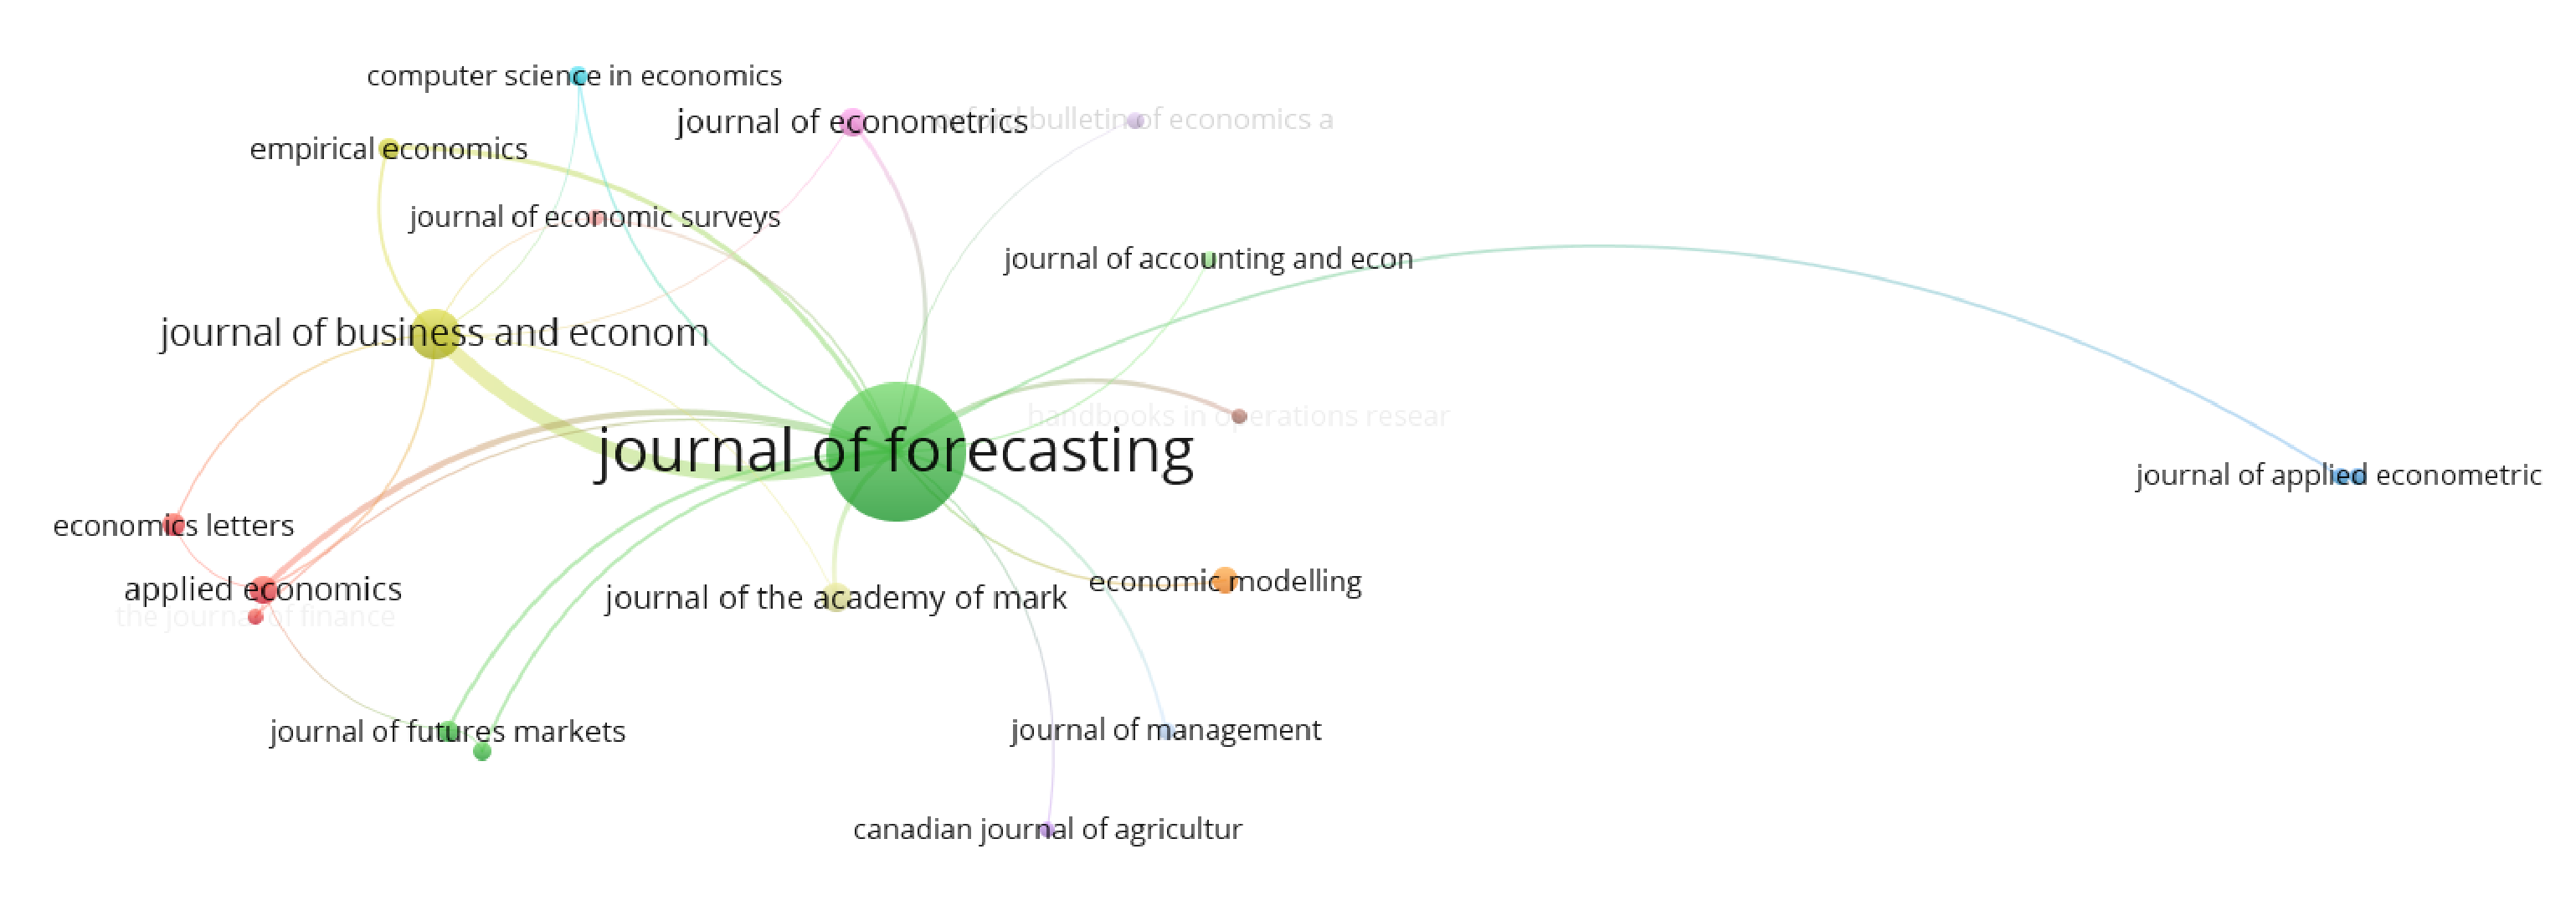
\includegraphics[width=\textwidth]{fig.23.eps}
\caption{JF journal citation network in Social Sciences}
\end{figure}

\tablez

\noindent B5: JF journal citation network in Environmental Science

20 Journals that have no less than 10 publications and 150 citations are
selected to map the JF journal citation network in Environmental
Science. Four parameters are clusters (7), local links (81), link
strength (861), and items (20).

\newpage

\begin{figure}[htbp]
\centering
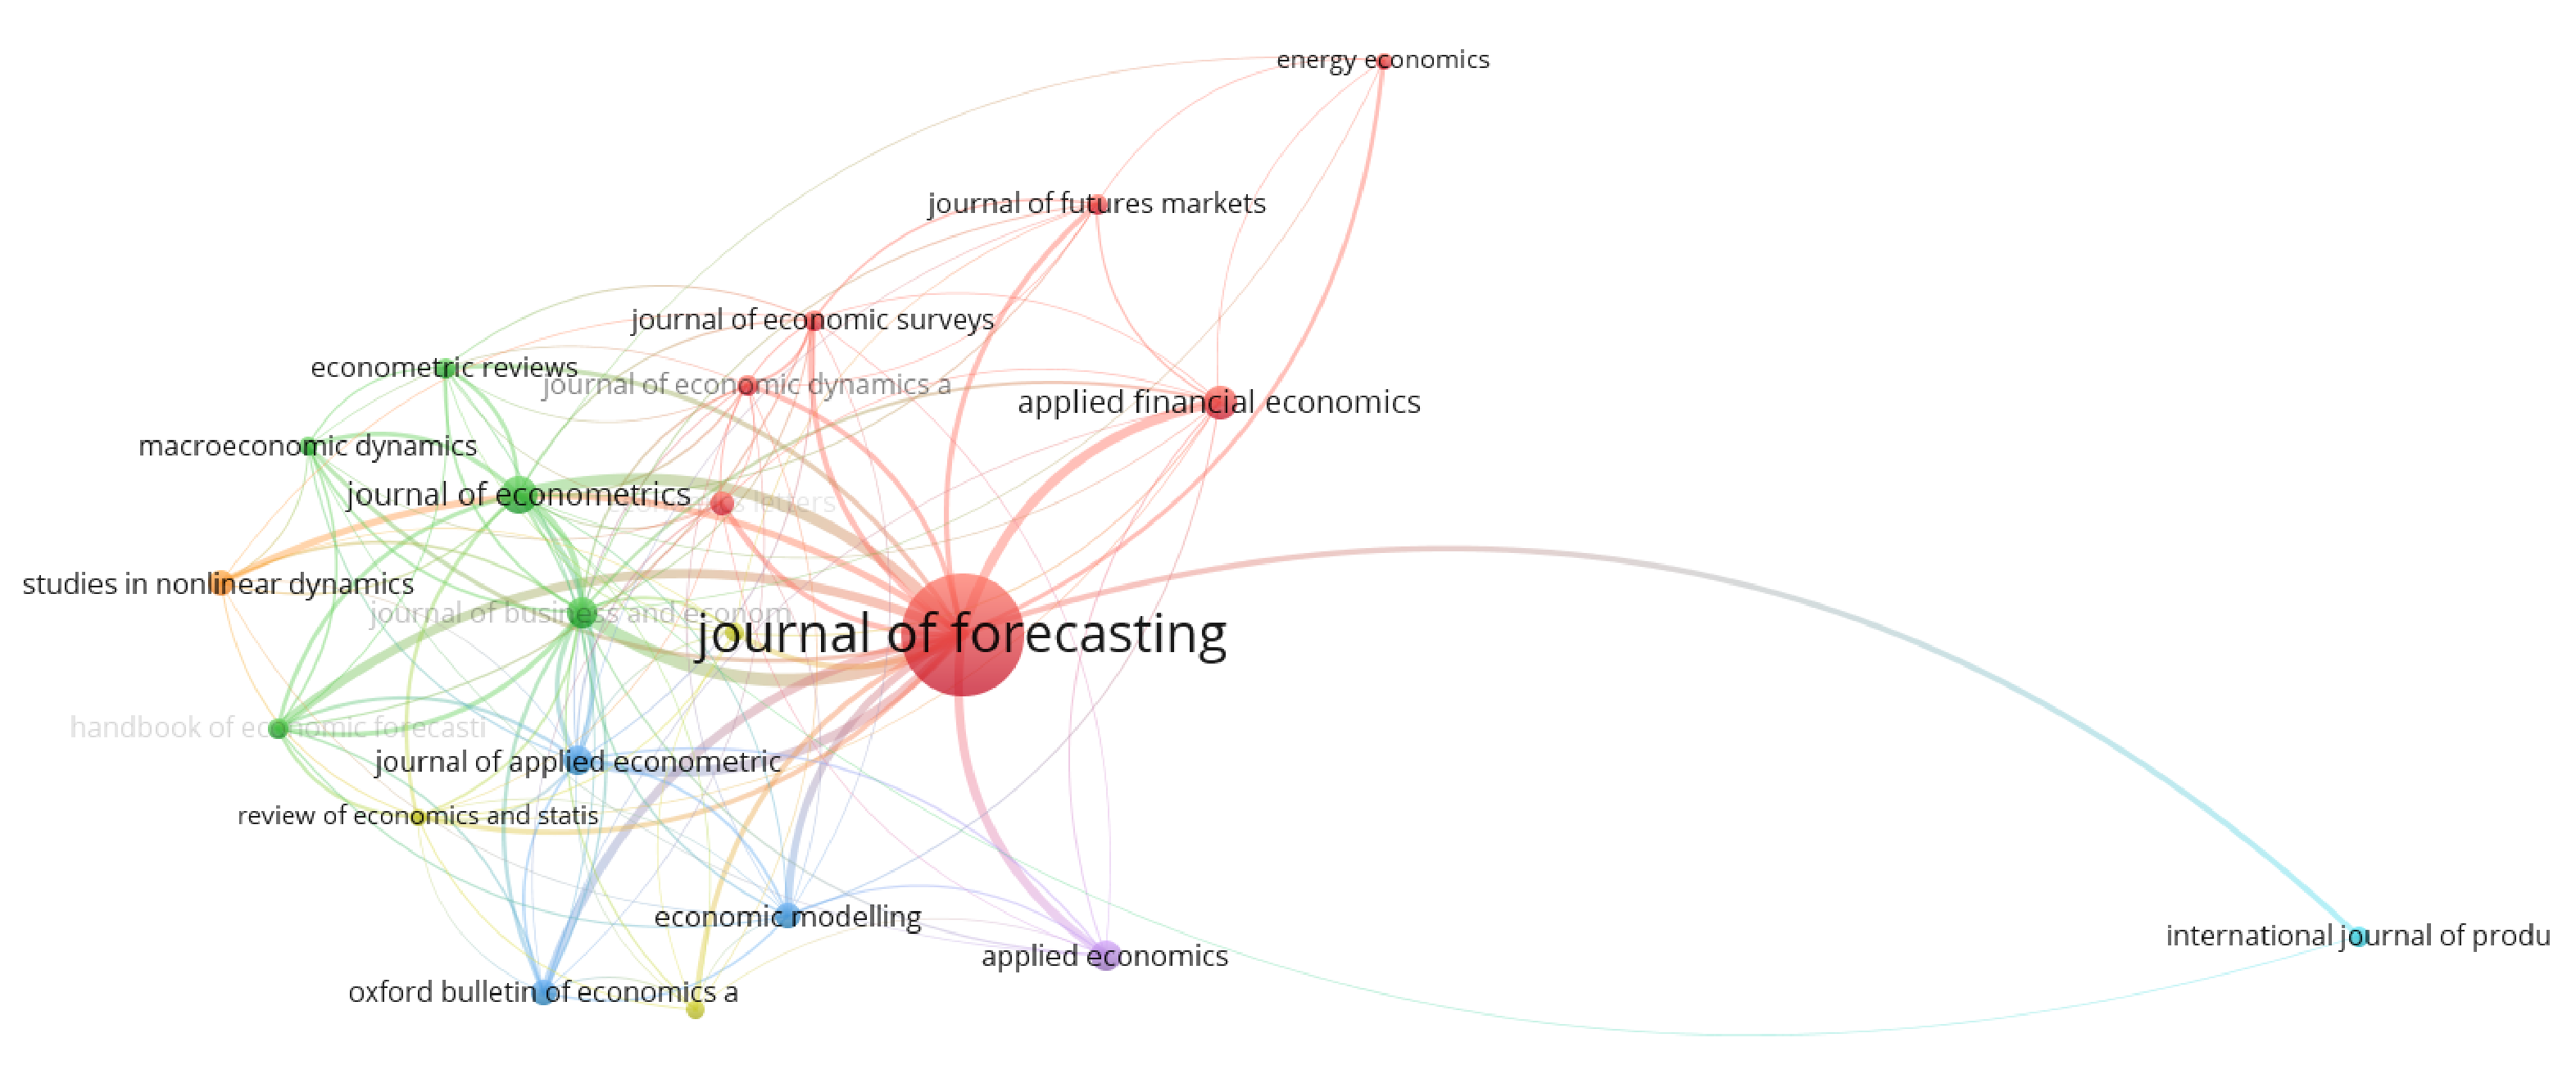
\includegraphics[width=\textwidth]{fig.24.eps}
\caption{JF journal citation network in Environmental Science}
\end{figure}

\tablezz

\noindent B6: JF journal citation network in Energy

20 Journals that have no less than 5 publications and 30 citations are
selected to map the JF journal citation network in Energy. Four
parameters are clusters (5), local links (96), link strength (793), and
items (20).

\newpage

\begin{figure}[htbp]
\centering
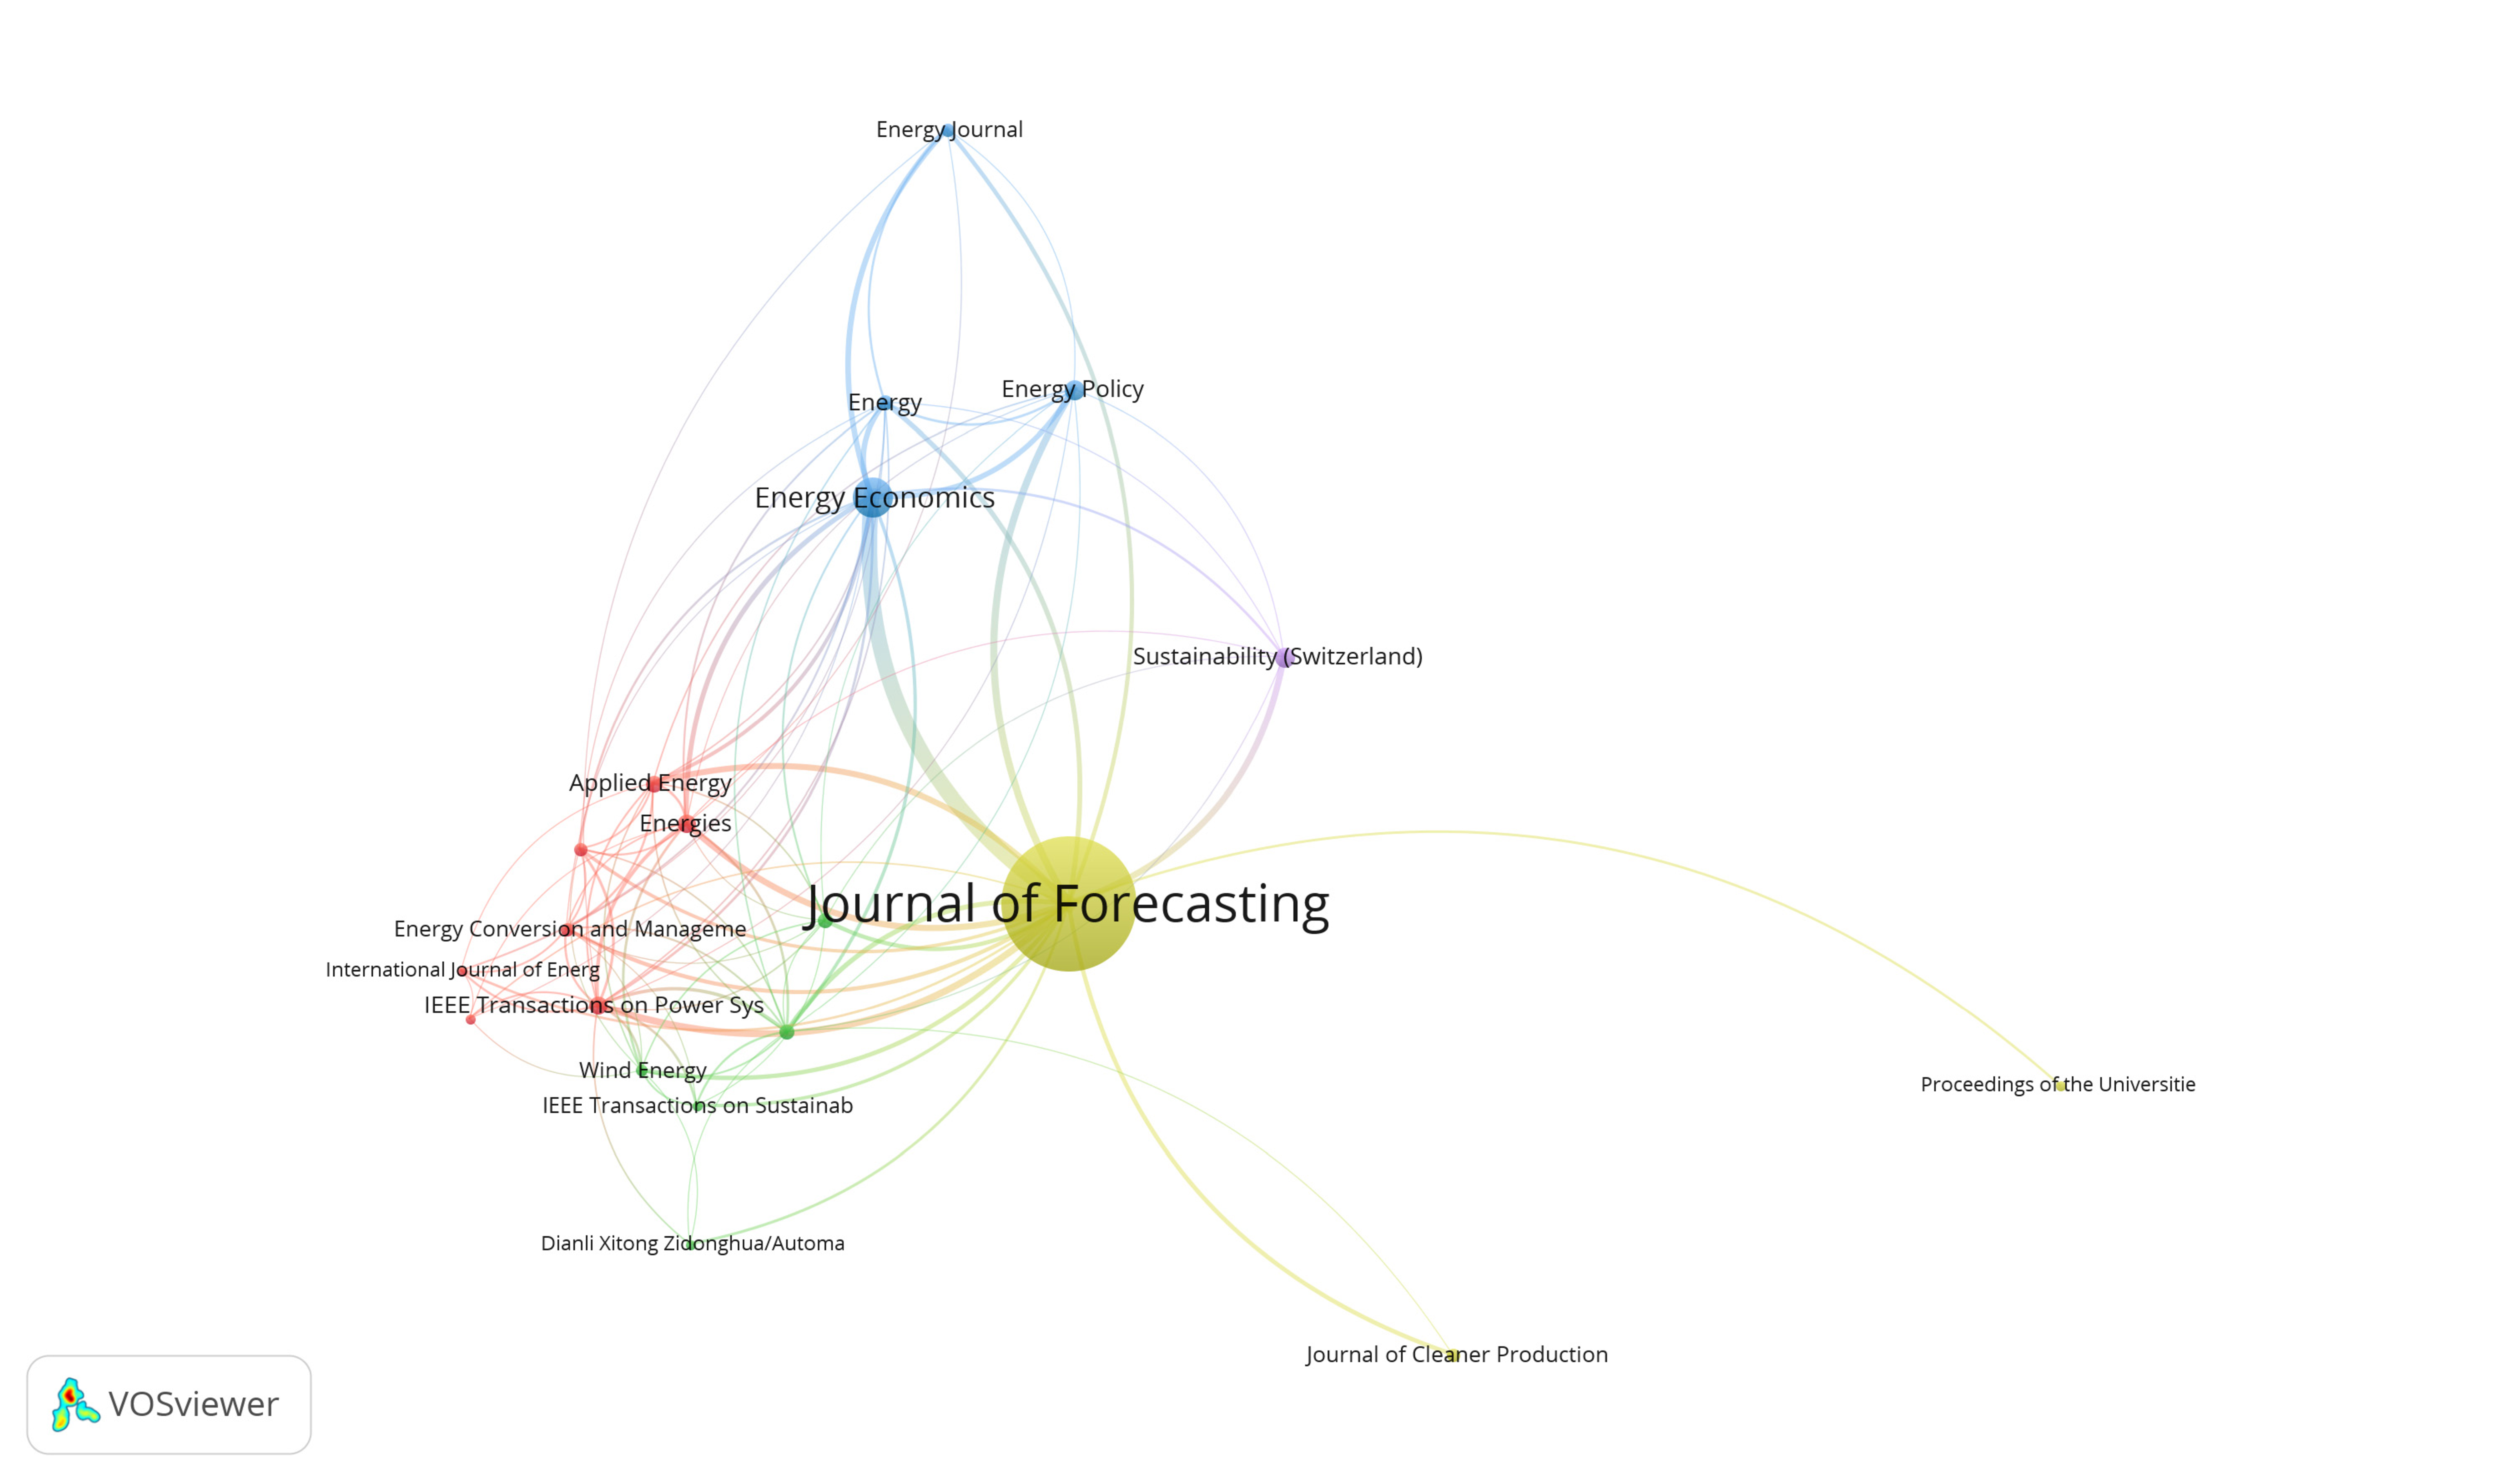
\includegraphics[width=\textwidth]{fig.25.eps}
\caption{JF journal citation network in Energy}
\end{figure}

\tablezzz

\noindent B7: JF journal citation network in Earth and Planetary
Sciences

20 Journals that have no less than 4 publications and 70 citations are
selected to map the JF journal citation network in Earth and Planetary
Sciences. Four parameters are clusters (6), local links (74), link
strength (608), and items (20).

\begin{figure}[htbp]
\centering
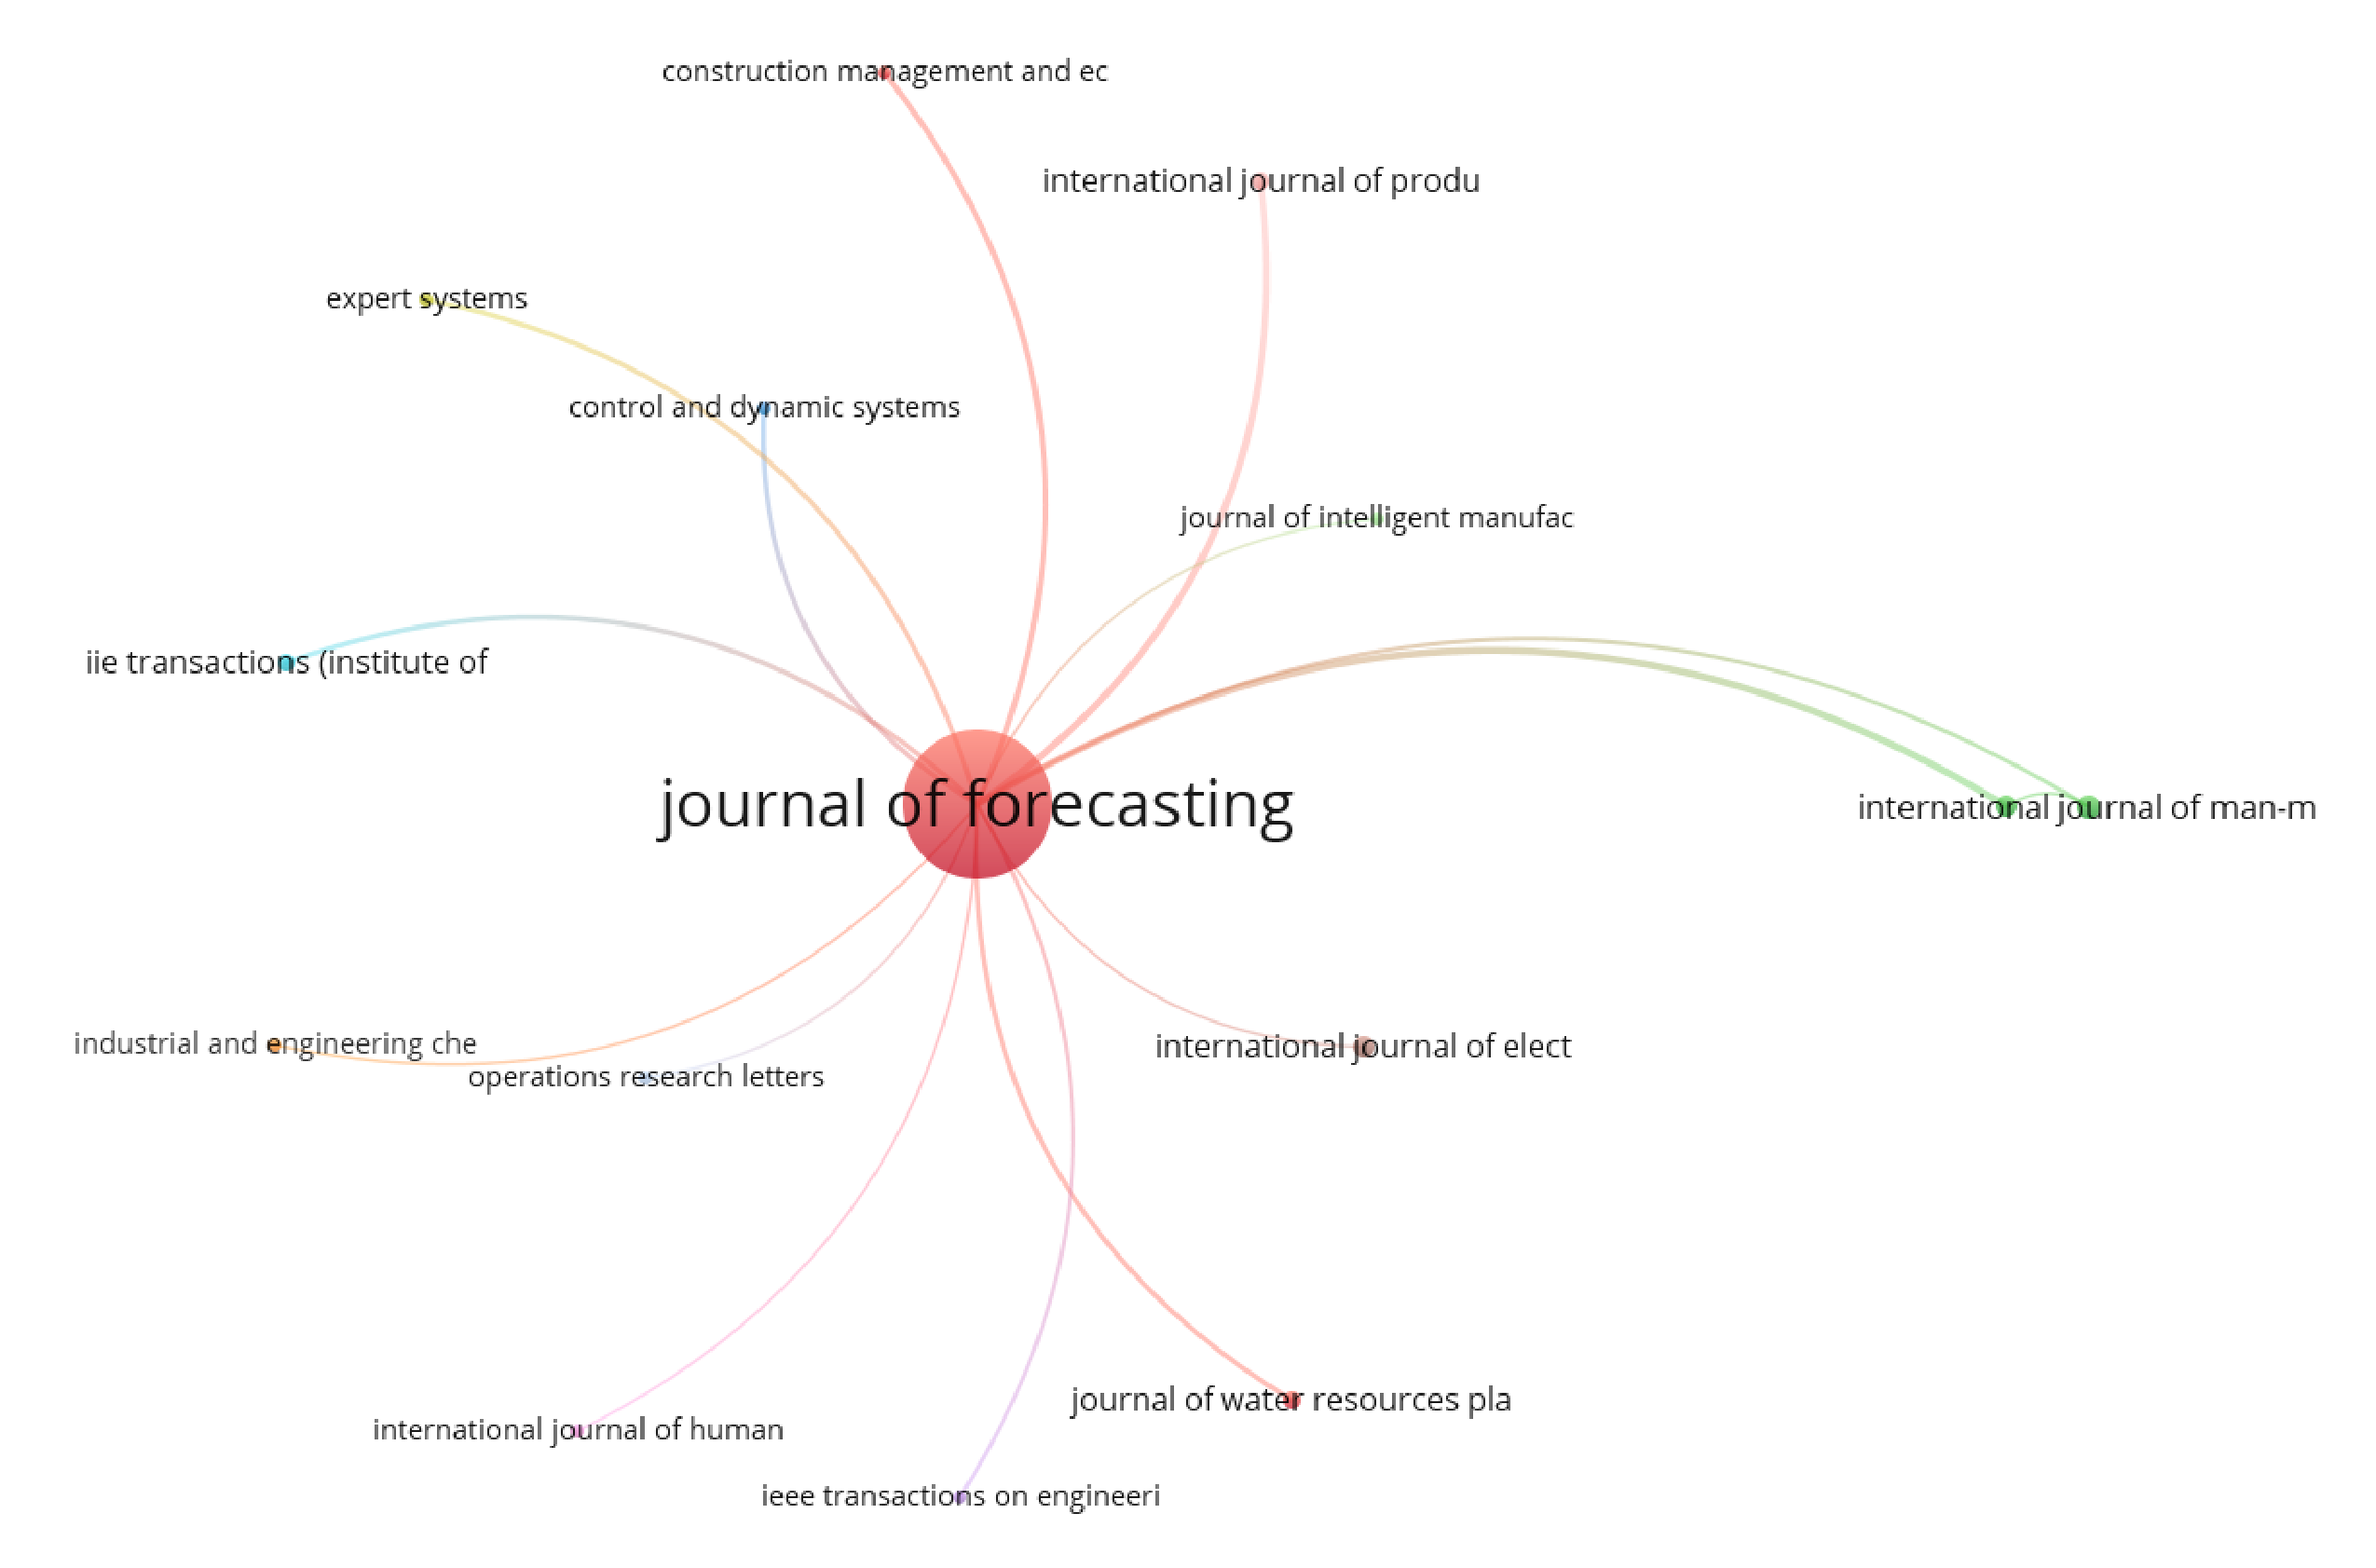
\includegraphics[width=\textwidth]{fig.26.eps}
\caption{JF journal citation network in Earth and Planetary Sciences}
\end{figure}

\tablezzzz

\section*{References}\label{references}
\addcontentsline{toc}{section}{References}

\hypertarget{refs}{}
\hypertarget{ref-Armstrong1992}{}
Armstrong, J. Scott, and Fred Collopy. 1992. ``Error Measures for
Generalizing About Forecasting Methods: Empirical Comparisons ☆.''
\emph{International Journal of Forecasting} 8 (1): 69--80.

\hypertarget{ref-Booth2006}{}
Booth, Heather. 2006. ``Demographic Forecasting: 1980 to 2005 in
Review.'' \emph{International Journal of Forecasting} 22 (3): 547--81.

\hypertarget{ref-Brown1993}{}
Brown, Lawrence D. 1993. ``Earnings Forecasting Research: Its
Implications for Capital Markets Research.'' \emph{International Journal
of Forecasting} 9 (3): 331--35.

\hypertarget{ref-Calma2016A}{}
Calma, Angelito, and Martin Davies. 2016. ``Academy of Management
Journal, 1958--2014: A Citation Analysis.'' \emph{Scientometrics} 108
(2): 959--75.

\hypertarget{ref-Clark2006}{}
Clark, Todd E., and Kenneth D. West. 2006. ``Approximately Normal Tests
for Equal Predictive Accuracy in Nested Models.'' \emph{Journal of
Econometrics} 138 (1): 291--311.

\hypertarget{ref-Clemen1989Combining}{}
Clemen, Robert T. 1989. ``Combining Forecasts: A Review and Annotated
Bibliography.'' \emph{International Journal of Forecasting} 5 (4):
559--83.

\hypertarget{ref-Conejo2005}{}
Conejo, Antonio J., Javier Contreras, Rosa Espínola, and Miguel A.
Plazas. 2005. ``Forecasting Electricity Prices for a Day-Ahead
Pool-Based Electric Energy Market.'' \emph{International Journal of
Forecasting} 21 (3): 435--62.

\hypertarget{ref-Crone2011Advances}{}
Crone, Sven F., Michèle Hibon, and Konstantinos Nikolopoulos. 2011.
``Advances in Forecasting with Neural Networks? Empirical Evidence from
the Nn3 Competition on Time Series Prediction.'' \emph{International
Journal of Forecasting} 27 (3): 635--60.

\hypertarget{ref-Darbellay2000}{}
Darbellay, Georges A., and Marek Slama. 2000. ``Forecasting the
Short-Term Demand for Electricity : Do Neural Networks Stand a Better
Chance?'' \emph{International Journal of Forecasting} 16 (1): 71--83.

\hypertarget{ref-Diebold2012}{}
Diebold, Francis X., and Kamil Yilmaz. 2012. ``Better to Give Than to
Receive: Predictive Directional Measurement of Volatility Spillovers.''
\emph{International Journal of Forecasting} 28 (1): 57--66.

\hypertarget{ref-Eck2009How}{}
Eck, Nees Jan Van, and Ludo Waltman. 2009. ``How to Normalize
Cooccurrence Data? An Analysis of Some Well-Known Similarity Measures.''
\emph{Journal of the American Society for Information Science and
Technology} 60 (8): 1635--51.

\hypertarget{ref-Fildes2006The}{}
Fildes, Robert. 2006. ``The Forecasting Journals and Their Contribution
to Forecasting Research: Citation Analysis and Expert Opinion.''
\emph{International Journal of Forecasting} 22 (3): 415--32.

\hypertarget{ref-Fildes2009}{}
Fildes, Robert, Paul Goodwin, Michael Lawrence, and Konstantinos
Nikolopoulos. 2009. ``Effective Forecasting and Judgmental Adjustments:
An Empirical Evaluation and Strategies for Improvement in Supply-Chain
Planning.'' \emph{International Journal of Forecasting} 25 (1): 3--23.

\hypertarget{ref-Freeman1977}{}
Freeman, Linton C. 1977. ``A Set of Measures of Centrality Based on
Betweenness.'' \emph{Sociometry} 40 (1): 35--41.

\hypertarget{ref-Gardner2006}{}
Gardner, Everette S. 2006. ``Exponential Smoothing: The State of the
Art---Part Ii.'' \emph{International Journal of Forecasting} 22 (4):
637--66.

\hypertarget{ref-Giacomini2006}{}
Giacomini, Raffaella., and Halbert. White. 2006. ``Tests of Conditional
Predictive Ability.'' \emph{Econometrica} 74 (6): 1545--78.

\hypertarget{ref-Giannone2008}{}
Giannone, Domenico, Lucrezia Reichlin, and David Small. 2008.
``Nowcasting: The Real-Time Informational Content of Macroeconomic
Data.'' \emph{Journal of Monetary Economics} 55 (4): 665--76.

\hypertarget{ref-Gooijer200625}{}
Gooijer, Jan G. De, and Rob J. Hyndman. 2006. ``25 Years of Time Series
Forecasting.'' \emph{Monash Econometrics \& Business Statistics Working
Papers} 22 (3): 443--73.

\hypertarget{ref-Hansen2011The}{}
Hansen, Peter R., Asger Lunde, and James M. Nason. 2011. ``The Model
Confidence Set.'' \emph{Econometrica} 79 (2): 453--97.

\hypertarget{ref-Harvey1997Testing}{}
Harvey, David, Stephen Leybourne, and Paul Newbold. 1997. ``Testing the
Equality of Prediction Mean Squared Errors.'' \emph{International
Journal of Forecasting} 13 (2): 281--91.

\hypertarget{ref-Holt2004}{}
Holt, Charles C. 2004. ``Forecasting Seasonals and Trends by
Exponentially Weighted Moving Averages.'' \emph{International Journal of
Forecasting} 20 (1): 5--10.

\hypertarget{ref-Hong2014}{}
Hong, Tao, Pierre Pinson, and Shu Fan. 2014. ``Global Energy Forecasting
Competition 2012.'' \emph{International Journal of Forecasting} 30 (2):
357--63.

\hypertarget{ref-Hong2016}{}
Hong, Tao, Pierre Pinson, Shu Fan, Hamidreza Zareipour, Alberto
Troccoli, and Rob J. Hyndman. 2016. ``Probabilistic Energy Forecasting:
Global Energy Forecasting Competition 2014 and Beyond.''
\emph{International Journal of Forecasting} 32 (3): 896--913.

\hypertarget{ref-Hyndman2006Another}{}
Hyndman, Rob J., and Anne B. Koehler. 2006. ``Another Look at Measures
of Forecast Accuracy.'' \emph{International Journal of Forecasting} 22
(4): 679--88.

\hypertarget{ref-Hyndman2000}{}
Hyndman, Rob J., Anne B. Koehler, Ralph D. Snyder, and Simone Grose.
2000. ``A State Space Framework for Automatic Forecasting Using
Exponential Smoothing Methods.'' \emph{Monash Econometrics \& Business
Statistics Working Papers} 18 (3): 439--54.

\hypertarget{ref-Kleinberg2003}{}
Kleinberg, J. 2003. ``Bursty and Hierarchical Structure in Streams.''
\emph{Data Mining and Knowledge Discovery} 7 (4): 373--97.

\hypertarget{ref-Lawrence2006Judgmental}{}
Lawrence, Michael, Paul Goodwin, Marcus O'Connor, and Dilek ?nkal. 2006.
``Judgmental Forecasting: A Review of Progress over the Last 25 Years.''
\emph{International Journal of Forecasting} 22 (3): 493--518.

\hypertarget{ref-Leydesdorff2014Interdisciplinarity}{}
Leydesdorff, Loet, and Robert L. Goldstone. 2014. ``Interdisciplinarity
at the Journal and Specialty Level: The Changing Knowledge Bases of the
Journal Cognitive Science.'' \emph{Journal of the Association for
Information Science \& Technology} 65 (1): 164--77.

\hypertarget{ref-Makridakis2000The}{}
Makridakis, Spyros, and Michèle Hibon. 2000. ``The M3-Competition:
Results, Conclusions and Implications.'' \emph{International Journal of
Forecasting} 16 (4): 451--76.

\hypertarget{ref-Meriguxf32015A}{}
Merigó, José M., Alicia Mas-Tur, Norat Roig-Tierno, and Domingo
Ribeiro-Soriano. 2015. ``A Bibliometric Overview of the Journal of
Business Research Between 1973 and 2014.'' \emph{Journal of Business
Research} 68 (12): 2645--53.

\hypertarget{ref-Porter1985An}{}
Porter, A. L., and D. E. Chubin. 1985. ``An Indicator of
Cross-Disciplinary Research.'' \emph{Scientometrics} 8 (3-4): 161--76.

\hypertarget{ref-Rowe1999The}{}
Rowe, G., and G. Wright. 1999. ``The Delphi Technique as a Forecasting
Tool: Issues and Analysis.'' \emph{International Journal of Forecasting}
15 (4): 353--75.

\hypertarget{ref-Shi2018Does}{}
Shi, Shunshun, Wenyu Zhang, Shuai Zhang, and Jie Chen. 2018. ``Does
Prestige Dimension Influence the Interdisciplinary Performance of
Scientific Entities in Knowledge Flow? Evidence from the E-Government
Field.'' \emph{Scientometrics} 117 (2): 1237--64.

\hypertarget{ref-Taylor2006}{}
Taylor, James W., Lilian M. De Menezes, and Patrick E. Mcsharry. 2006.
``A Comparison of Univariate Methods for Forecasting Electricity Demand
up to a Day Ahead.'' \emph{International Journal of Forecasting} 22 (1):
1--16.

\hypertarget{ref-Thomas2000A}{}
Thomas, Lyn C. 2000. ``A Survey of Credit and Behavioural Scoring:
Forecasting Financial Risk of Lending to Consumers.''
\emph{International Journal of Forecasting} 16 (2): 149--72.

\hypertarget{ref-Timmermann2006}{}
Timmermann, Allan. 2006. ``Forecast Combinations.'' \emph{Handbook of
Economic Forecasting} 1: 135--96.

\hypertarget{ref-Weron2014Electricity}{}
Weron, Rafał. 2014. ``Electricity Price Forecasting: A Review of the
State-of-the-Art with a Look into the Future.'' \emph{International
Journal of Forecasting} 30 (4): 1030--81.

\hypertarget{ref-Wichaisri2018Trends}{}
Wichaisri, Sooksiri, and Apichat Sopadang. 2018. ``Trends and Future
Directions in Sustainable Development.'' \emph{Sustainable Development}
26 (1): 1--17.

\hypertarget{ref-Witt1995Forecasting}{}
Witt, Stephen F., and Christine A. Witt. 1995. ``Forecasting Tourism
Demand: A Review of Empirical Research.'' \emph{International Journal of
Forecasting} 11 (3): 447--75.

\hypertarget{ref-Yu2015A}{}
Yu, Dejian. 2015. ``A Scientometrics Review on Aggregation Operator
Research.'' \emph{Scientometrics} 105 (1): 115--33.

\hypertarget{ref-Yu2015Researching}{}
Yu, Dejian, and Shunshun Shi. 2015. ``Researching the Development of
Atanassov Intuitionistic Fuzzy Set: Using a Citation Network Analysis''
32: 189--98.

\hypertarget{ref-Yu2017Information}{}
Yu, Dejian, Zeshui Xu, Witold Pedrycz, and Wanru Wang. 2017.
``Information Sciences 1968-2016: A Retrospective Analysis with Text
Mining and Bibliometric.'' \emph{Information Sciences} 418: 2727--36.

\hypertarget{ref-Zhang1998}{}
Zhang, B. Eddy Patuwo, and Michael Y. Hu. 1998. ``Forecasting with
Artificial Neural Networks: The State of the Art.'' \emph{International
Journal of Forecasting} 14 (1): 35--62.

\end{document}


